%
% Manual.tex
% TAZ Manual main document formatting
%
% LulzBot TAZ User Manual
%
% Copyright (C) 2014 Aleph Objects, Inc.
%
% This document is licensed under the Creative Commons Attribution 4.0
% International Public License (CC BY-SA 4.0) by Aleph Objects, Inc.
%

%%% Images may be commented out to render more quickly
%%%
%%% Bug on ShareLaTeX: glossary and index are not rendering.
%%% https://sharelatex.tenderapp.com/help/discussions/questions/19378-glossaries-indices-and-speed


%%% MEMOIR CLASS %%%
\documentclass[twoside,12pt,openright,final,english]{memoir}
% Memoir Divisions: \book, \part, \chapter, \section, \subsection
% Fine divisions:   \subsubsection, \paragraph \subparagraph.
%%% END MEMOIR CLASS %%%

%%% PREAMBLE FONTS %%%
% For XeLaTeX
% http://www.ctan.org/pkg/fontspec
% http://mirrors.ctan.org/macros/latex/contrib/fontspec/fontspec.pdf
\usepackage{fontspec}
\defaultfontfeatures{Ligatures=TeX} % To support LaTeX quoting style
\setmainfont{lmroman12-regular.otf}

\usepackage[normalem]{ulem} % underline
%%% END PREAMBLE FONTS %%%

\usepackage{float}
\usepackage{comment}
\usepackage{graphicx}
\usepackage{epstopdf}
% For full size print graphics
% Note, these images haven't been uploaded yet
%\graphicspath{{./images-original/}}
% For web quality output
% Note, some of these "web" images are much larger than they should be
%%% Images commented out to render more quickly
\graphicspath{{./images-1600x1200/}}

\makeindex
%%% GLOSSARY
\makeglossary
%%% END GLOSSARY

\usepackage{color}
\usepackage[usenames,dvipsnames,svgnames,table]{xcolor}

\usepackage[english]{babel}
\usepackage{datetime}

%%% PAGE, STOCK, AND MARGIN SIZE %%%
% Lulu 7.44 x 9.68"   18.90 x 24.58cm
\setstocksize{24.58cm}{18.90cm} % { height }{ width }
\settrimmedsize{\stockheight}{\stockwidth}{*}

%\settypeblocksize{ height }{ width }{ ratio }
\settypeblocksize{19.0cm}{*}{*}

%\setlrmarginsandblock{ spine }{ edge }{ ratio }
% make the spine have more space than outer edge
\setlrmarginsandblock{*}{2.5cm}{1.2}

% \setulmargins{ upper }{ lower }{ ratio }
\setulmargins{2.0cm}{*}{*}

% \setheadfoot{ headheight }{ footskip }
\setheadfoot{12pt}{2cm}

\checkandfixthelayout[fixed]
%%% END PAGE, STOCK, AND MARGIN SIZE %%%

%%% INCLUDED FILES %%%
% select which chapters to render:
\newif\iftitle\titletrue
\newif\ifcopyright\copyrighttrue
\newif\ifwarnings\warningstrue %true
\newif\ifsetup\setupfalse %false
\newif\ifslicer\slicertrue %true
\newif\ifsoftware\softwaretrue %true
\newif\iffilament\filamentfalse %false
\newif\iffirstprint\firstprintfalse %false
\newif\ifglcd\glcdtrue %true
\newif\ifmaintenance\maintenancetrue %true
\newif\ifadvanced\advancedtrue %true
\newif\iffaq\faqfalse %false - Not yet written
\newif\iftroubleshooting\troubleshootingfalse %false - Not yet written
\newif\ifsource\sourcetrue %true
\newif\ifsupport\supporttrue %true
\newif\ifcontact\contacttrue %true
\newif\ifcolophon\colophontrue %true
%% or just render everything:
\newif\ifrendereverything\rendereverythingfalse
\ifrendereverything \titletrue \copyrighttrue \warningstrue \setuptrue \slicertrue \softwaretrue \filamenttrue \firstprinttrue \maintenancetrue \advancedtrue \faqtrue \troubleshootingtrue \colophontrue \fi
%%% END INCLUDED FILES %%%

\setcounter{secnumdepth}{3}
\setcounter{tocdepth}{3}

\usepackage[english]{babel}
\usepackage{ucs}

%%% PDFLATEX %%%
\usepackage{etex}

% http://mirrors.ctan.org/macros/latex/contrib/microtype/microtype.pdf
\usepackage[protrusion,babel,final]{microtype}
% This may need to be disabled for XeTeX
%\usepackage[utf8x]{inputenc}

%\usepackage{eledmac}
%% Use ledmac for compiling on debian
\usepackage{ledmac}

%%% PAGE STYLE %%%
\makepagestyle{jebstyle}
\pagestyle{jebstyle}
\makeevenhead{jebstyle}{}{\hspace{2em}\itshape\small\leftmark}{} % KLUDGE
\makeoddhead{jebstyle}{}{\scshape\small\rightmark}{}
\makeevenfoot{jebstyle}{}{\hspace{2em}\thepage}{} % KLUDGE
\makeoddfoot{jebstyle}{}{\thepage}{}
%%% END 

%%% jebinski CHAPTER STYLE %%%
\makechapterstyle{jebinski}{%
% Clear out the chapter name (e.g. capítulo)
  \renewcommand*{\printchaptername}{}
% Clear out the chapter number
  \renewcommand*{\printchapternum}{}
% Set chapter font
  \renewcommand*{\chaptitlefont}{\normalfont\large\scshape}
  \renewcommand*{\printchaptertitle}[1]{%
     \hrule\vskip\onelineskip \centering \chaptitlefont{##1}\par}
  \renewcommand*{\afterchaptertitle}{\vskip\onelineskip \hrule\vskip
     \afterchapskip}
}
%%% END jebinski CHAPTER STYLE %%%

%%% FORMATTING KLUDGES %%%
% fewer overfull lines compared with \fussy and fewer obvious
% large interword spaces than with \sloppy.
\midsloppy
% "fix" for Overfull \hbox
%\emergencystretch=8pt
\setlength{\emergencystretch}{3em}
% \tolerance is a paragraph parameter, probably ignored here
\tolerance=5000 % allow looser spacing 
%\tolerance=95000 % allow waaay looser spacing 
% 10000 almost prevents hyphenation. What's default?
\hyphenpenalty=500 % 500 seems reasonable
%the default \flushbottom
%\sloppypar
\setlength{\topskip}{1.6\topskip}
\checkandfixthelayout
%\sloppybottom
\raggedbottom
%%%%%%%% WIDOWS AND ORPHANS %%%%%%%%%%%
\widowpenalty=10000
\clubpenalty=10000
%%%%%%%% END WIDOWS AND ORPHANS %%%%%%%%%%%
%%% END FORMATTING KLUDGES %%%

%%% FOOTNOTES %%%
% no horizontal rule before footnotes:
\let\oldfootnoterule\footnoterule
\renewcommand*{\footnoterule}{}
% This indents the footnote, or it lines up too far to the
% left on the spanish side. The right page note should really
% move over more to the left
% KLUDGE
\setlength{\footmarkwidth}{3.5em}
%%% END FOOTNOTES %%%

%%% Fancy dings %%%
\usepackage{pifont}

%%% DEBUG %%%
%\showoutput
%\typeoutlayout
%\typeoutstandardlayout
%%% END DEBUG %%%

%%% END OF PREAMBLE %%%

\begin{document}

%%% BEGIN FRONT MATTER %%%
\frontmatter

% Set page numbers to lowercase roman numerals, and reset the count to 1 (no *)
\pagenumbering{roman}

%%% TITLE PAGE %%%
% We want the title to be on the right hand page.
% If we pad a page, it gives us two with openright
\iftitle
{% clear the page style
\date {}
\thispagestyle{empty}
\begingroup
\centering 
%{\Huge \scshape TAZ User Manual}\\[\baselineskip]

\begin{center}
{\huge \scshape TAZ 2.0 User Manual}

\end{center}

\par


%\vspace*{0.1\textheight} 
%%% SET TITLE FONT
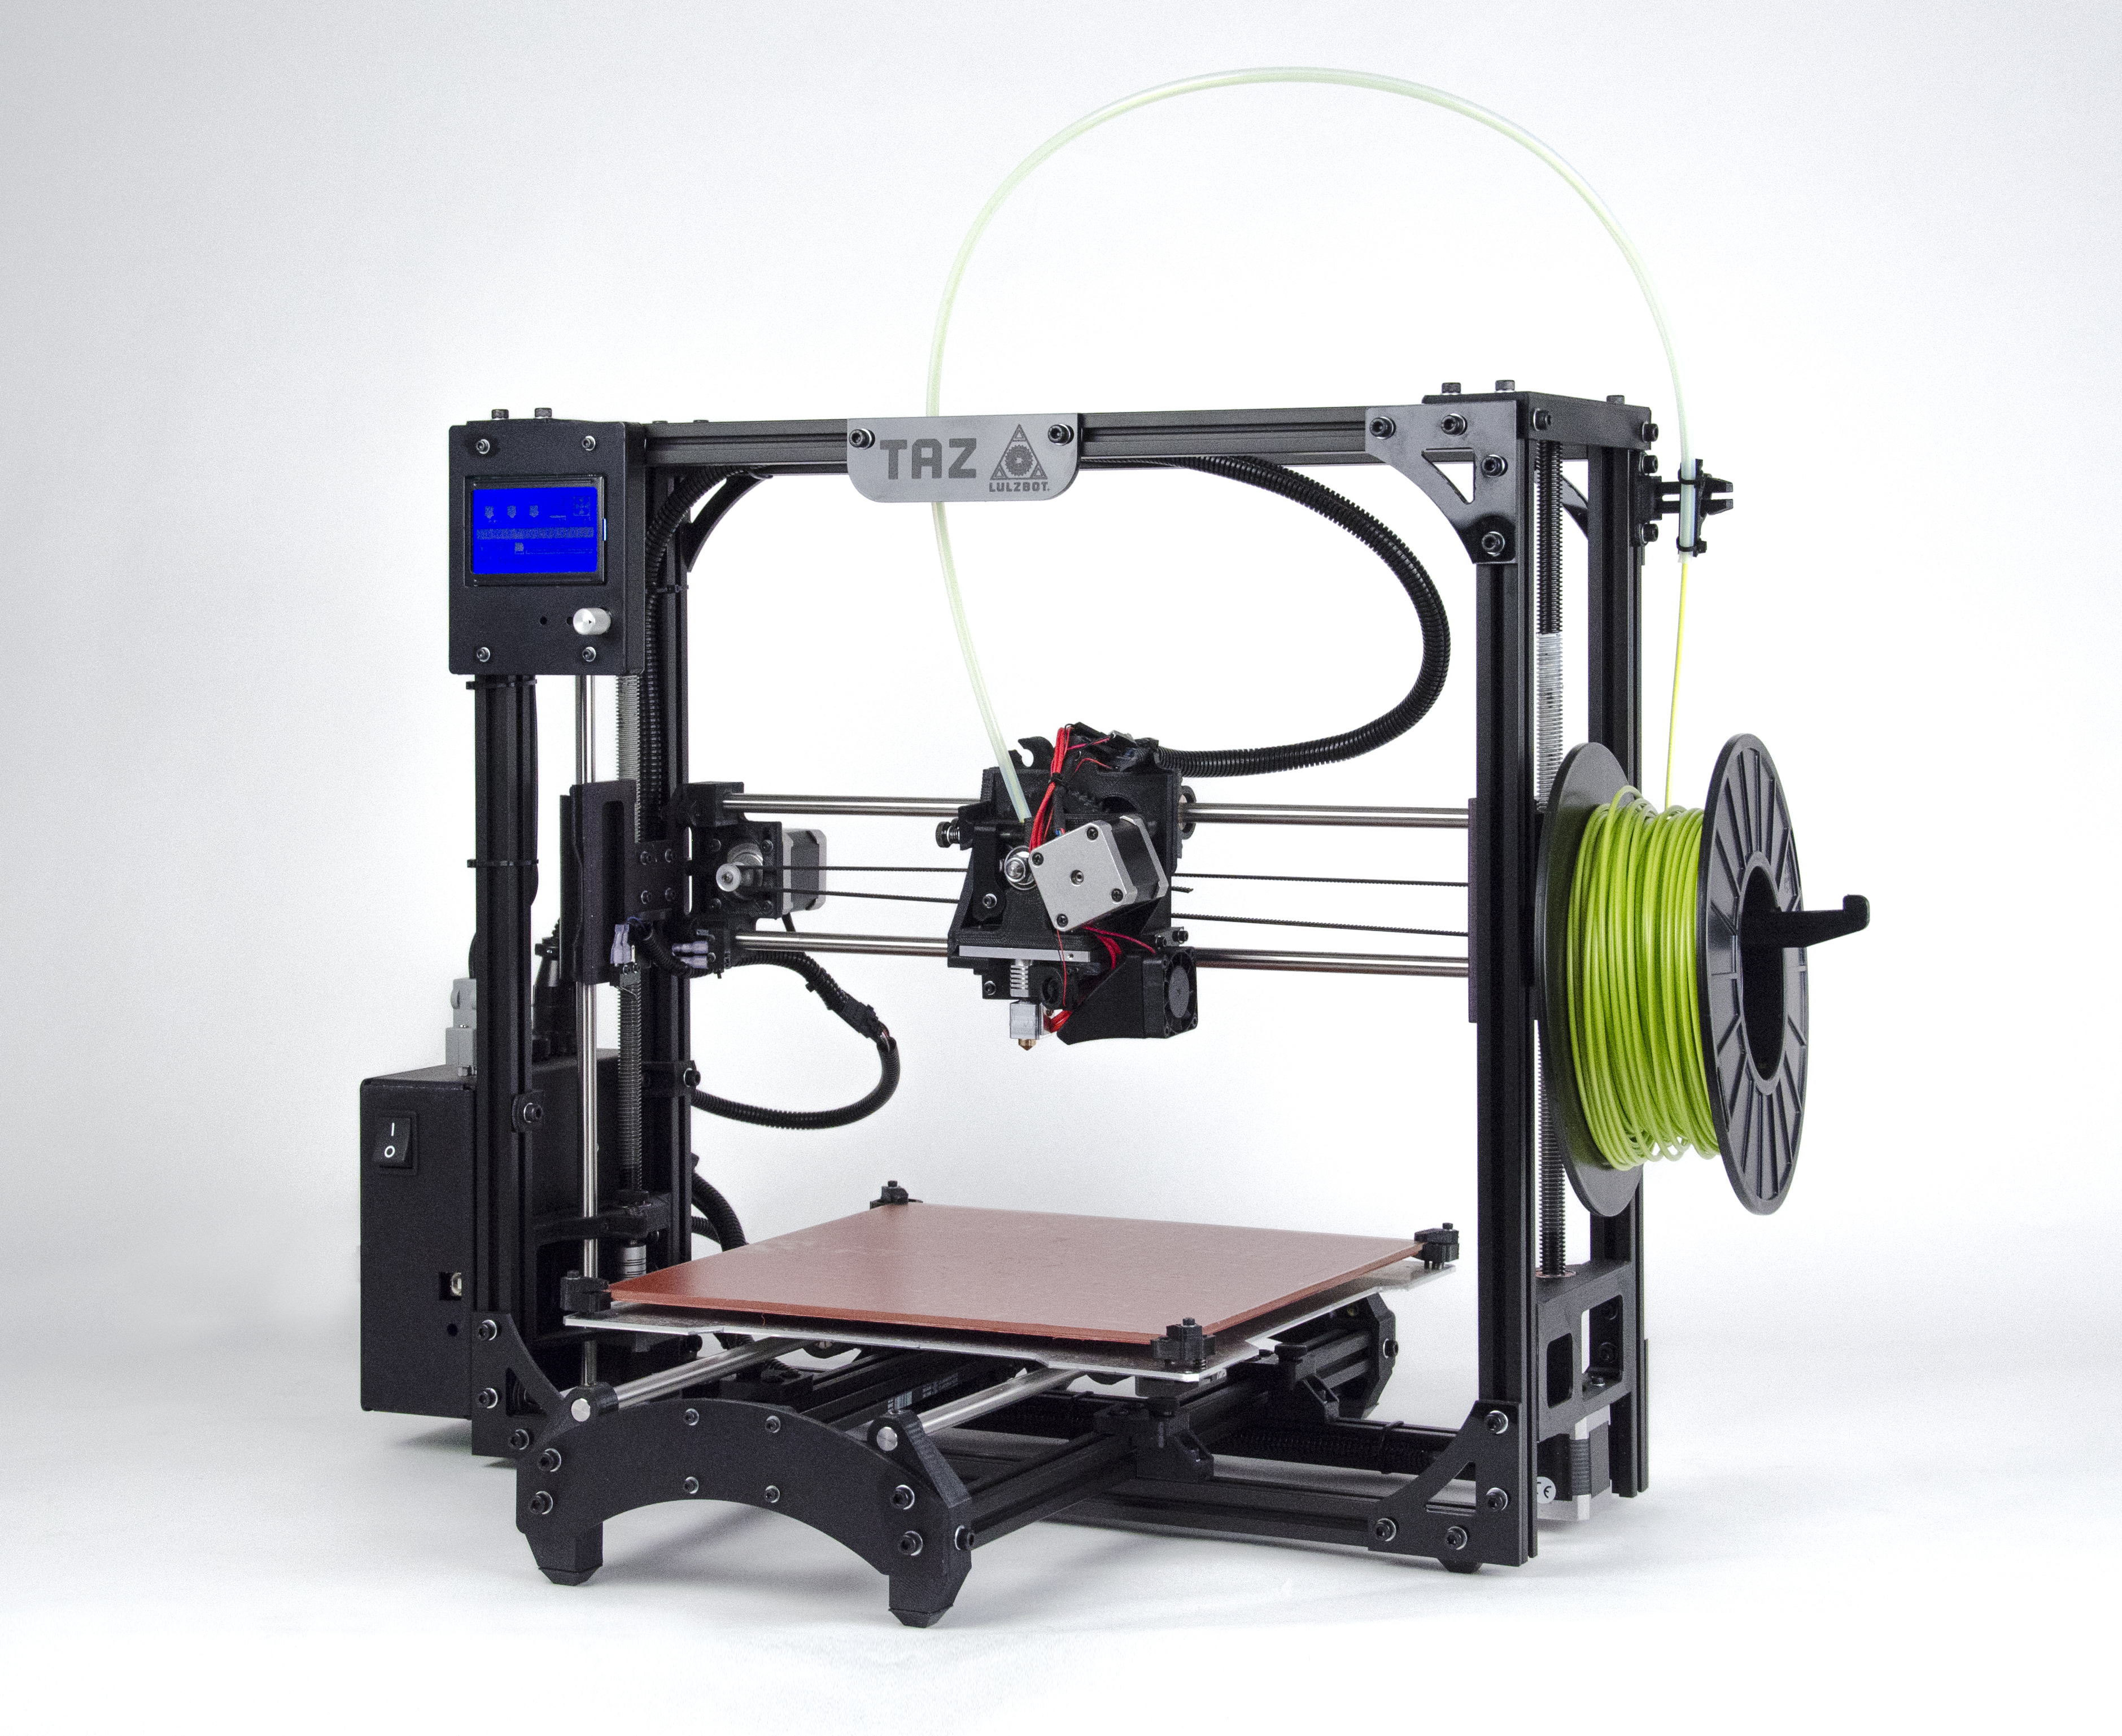
\includegraphics[keepaspectratio=true,angle=0,height=1.0\textheight,width=1.0\textwidth]{taz.jpg}

%\null\vfill
%\rule{0.4\textwidth}{0.4pt}
%\par
\begin{center}
\includegraphics[keepaspectratio=true,angle=0,height=0.25\textheight,width=0.25\textwidth]{Lulzbot_LogoTM_4c.eps}

{\large \itshape Aleph Objects, Inc.}
\end{center}
\endgroup
%\vspace*{0.1\textheight} 
%\newpage
%\clearpage

}
\fi
%%% END TITLE PAGE

%%% COPYRIGHT PAGE %%%
\ifcopyright
{\clearpage\null\vfill
\begingroup 
%\vfill\null 
\thispagestyle{empty}
\footnotesize\raggedright
\setlength{\parskip}{0.5\baselineskip}

\textbf{LulzBot\textsuperscript{\miniscule{\texttrademark}} TAZ 3 User Manual}

by Aleph Objects, Inc.

Copyright \copyright\ \the\year\ Aleph Objects, Inc.\par
Permission is granted to copy, distribute and\slash or modify 
this document under the terms of the
Creative Commons Attribution-ShareAlike 3.0 Unported license
(CC BY-SA 3.0).

Published by Aleph Objects, Inc., 626 W 66th Street, Loveland, Colorado, 80538 USA.

For more information, call +1-970-377-1111 or go to \texttt{www.LulzBot.com} and \texttt{www.AlephObjects.com}.

ISBN: 978-0-9893784-4-4
\hfill\texttt3.1.{\the\year\the\month\the\day}
\endgroup
\pagebreak{}
}
\fi
%%% END COPYRIGHT PAGE %%%


%%% TABLE OF CONTENTS ToC %%%
\maxtocdepth{section}
% Dots
% space between dots
\renewcommand{\cftchapterdotsep}{15}
% dot symbol (default is period)
\renewcommand{\cftdot}{\textperiodcentered}	% centered period
% Set space between each entry in ToC
\setlength{\cftbeforechapterskip}{5pt}  % 5pt % 3pt
\tableofcontents*
%%% END TABLE OF CONTENTS ToC %%%

%%% LIST OF FIGURES %%%
%\addtodef{\listoffigures}{\clearpage\pagestyle{lof}}{}
% Fit all of List of Figures on one page
\renewcommand*{\lofheadstart}{\vspace{1cm}}
\clearpage
\listoffigures*
%%% END LIST OF FIGURES %%%

%%% CHAPTER STYLE %%%
\chapterstyle{jebinski} % defined in preamble
\def\topblockvspace{0.11}


%%% WARNINGS %%%
\ifwarnings
\chapter{\emph{WARNINGS}\protect \\
{Safety Information}}
\thispagestyle{empty}
\markboth{WARNING!}{Be Safe!}
{%
% Warnings.tex
%
% LulzBot® TAZ User Manual
%
% Copyright (C) 2014 Aleph Objects, Inc.
%
% This document is licensed under the Creative Commons Attribution 4.0
% International Public License (CC BY-SA 4.0) by Aleph Objects, Inc.
%

\section{\texttt{Read Me First!}}
\index{warnings}
\index{hazards}
\textcolor{red}{READ THIS MANUAL COMPLETELY BEFORE UNPACKING AND POWERING UP YOUR PRINTER.}

\section{\texttt{Hazards and Warnings}}

Your LulzBot\textsuperscript{\miniscule{\textregistered}} TAZ 3D printer has motorized and heated parts.  Always be aware of possible hazards when the printer is operational.


\subsection{\textcolor{red}{Electric Shock Hazard}}
\index{electronics}
\index{wires}
\index{power supply}
Never open the electronics case when the printer is powered on. Before removing the electronics case cover always power down the printer and completely turn off and unplug the power supply. Allow the power supply to discharge for at least one minute.

\subsection{\textcolor{red}{Burn Hazard}}
\index{extruder}
\index{heater block}
\index{temperature}
\index{burns}
Never touch the extruder nozzle or heater block without first turning off the hot end and allowing it to completely cool down. The hot end can take up to 20 minutes to completely cool. Never touch recently extruded plastic. The plastic can stick to your skin and cause burns. The heated bed can reach high temperatures that are capable of causing burns.

\subsection{\textcolor{red}{Fire Hazard}}
Never place flammable materials or liquids on or near the printer when it is powered on or operational. Liquid acetone and vapors are extremely flammable.

\subsection{\textcolor{red}{Pinch Hazard}}

When the printer is operational take care to never put your fingers in any moving parts including belts, pulleys, or gears. Tie back long hair or clothing that can get caught in the moving parts of the printer.

\subsection{\textcolor{red}{Static Charge}}
\index{static}
Make sure to ground yourself before touching the printer, especially its electronics. Electrostatic discharge can damage electronic components. Ground yourself by touching a grounded source like your computer case.

\subsection{\textcolor{red}{Age Warning}}

For users under the age of 18, adult supervision is recommended. Beware of choking hazards around small children.

\subsection{\textcolor{red}{Modifications and Repairs Warning}}

At Aleph Objects, Inc.\textsuperscript{\miniscule{\textregistered}} we respect your freedom to modify your LulzBot\textsuperscript{\miniscule{\textregistered}} desktop 3D printer. However any modifications or attempted repairs that cause damage are not covered under the Warranty. Questions? Contact Technical Support by emailing support@lulzbot.com, or by calling +1-970-377-1111.

\subsection{\texttt{Federal Communications Commission Statement}}
\index{FCC}
Note: This equipment has been tested and found to comply with the limits for a Class A digital device, pursuant to part 15 of the FCC Rules. These limits are designed to provide reasonable protection against harmful interference when the equipment is operated in a commercial environment. This equipment generates, uses, and can radiate radio frequency energy and, if not installed and used in accordance with the instruction manual, may cause harmful interference to radio communications. Operation of this equipment in a residential area is likely to cause harmful interference in which case the user will be required to correct the interference at his own expense.

This device complies with part 15 class A of the FCC Rules. Operation is subject to the following two conditions:
\begin{enumerate}
\item This device may not cause harmful interference and
\item This device must accept any interference received, including interference that may cause undesired operation.
\end{enumerate}

\textcolor{red}{FCC Warning:}
\textcolor{red}{Changes or modifications not approved by the party responsible for compliance could void the users authority to operate the equipment.}



}
\fi
%%% END WARNINGS %%%

%%% END FRONTMATTER %%%
%%% BEGIN MAINMATTER %%%
\mainmatter*

% Set page numbering to arabic, but don't reset numbering (*)
\pagenumbering*{arabic}

%%% SETUP %%%
\ifsetup
\chapter{\emph{Setup Your Printer}}
\thispagestyle{empty}
\markboth{Setup Your Printer}{LulzBot\textsuperscript{\miniscule{\texttrademark}} TAZ User Manual}
{\begin{enumerate}
\item Your printer has been pre-calibrated and tested; however, after unpacking you will need to double check that everything is in order before you print.

\item You should set your printer on a stable, flat, and level surface large enough for extra space around the printer. Make sure your printer work space is clear of anything that could obstruct the movement of the printer. \textcolor{red}{Make sure there are no flammable fabrics or liquids near the printer space}. It is also best to not put your printer near a drafty window or air conditioner vent.

\index{end stops}
\item Check that the three mechanical end stops are aligned to contact with the respective ends. The mechanical end stops are small switches located at the home point of each axis.
(Fig. \ref{fig:axes}, page \pageref{fig:axes}; Fig. \ref{fig:xz_endstops}, page \pageref{fig:xz_endstops}; Fig. \ref{fig:y_endstop}, page \pageref{fig:y_endstop}).
\begin{figure}[hp]
\centering
\includegraphics[keepaspectratio=true,angle=0,height=0.4\textheight,width=1.0\textwidth]{axes.jpg}
\caption{Axes movement directions}
\label{fig:axes}
\end{figure}
\begin{figure}[hp]
\centering
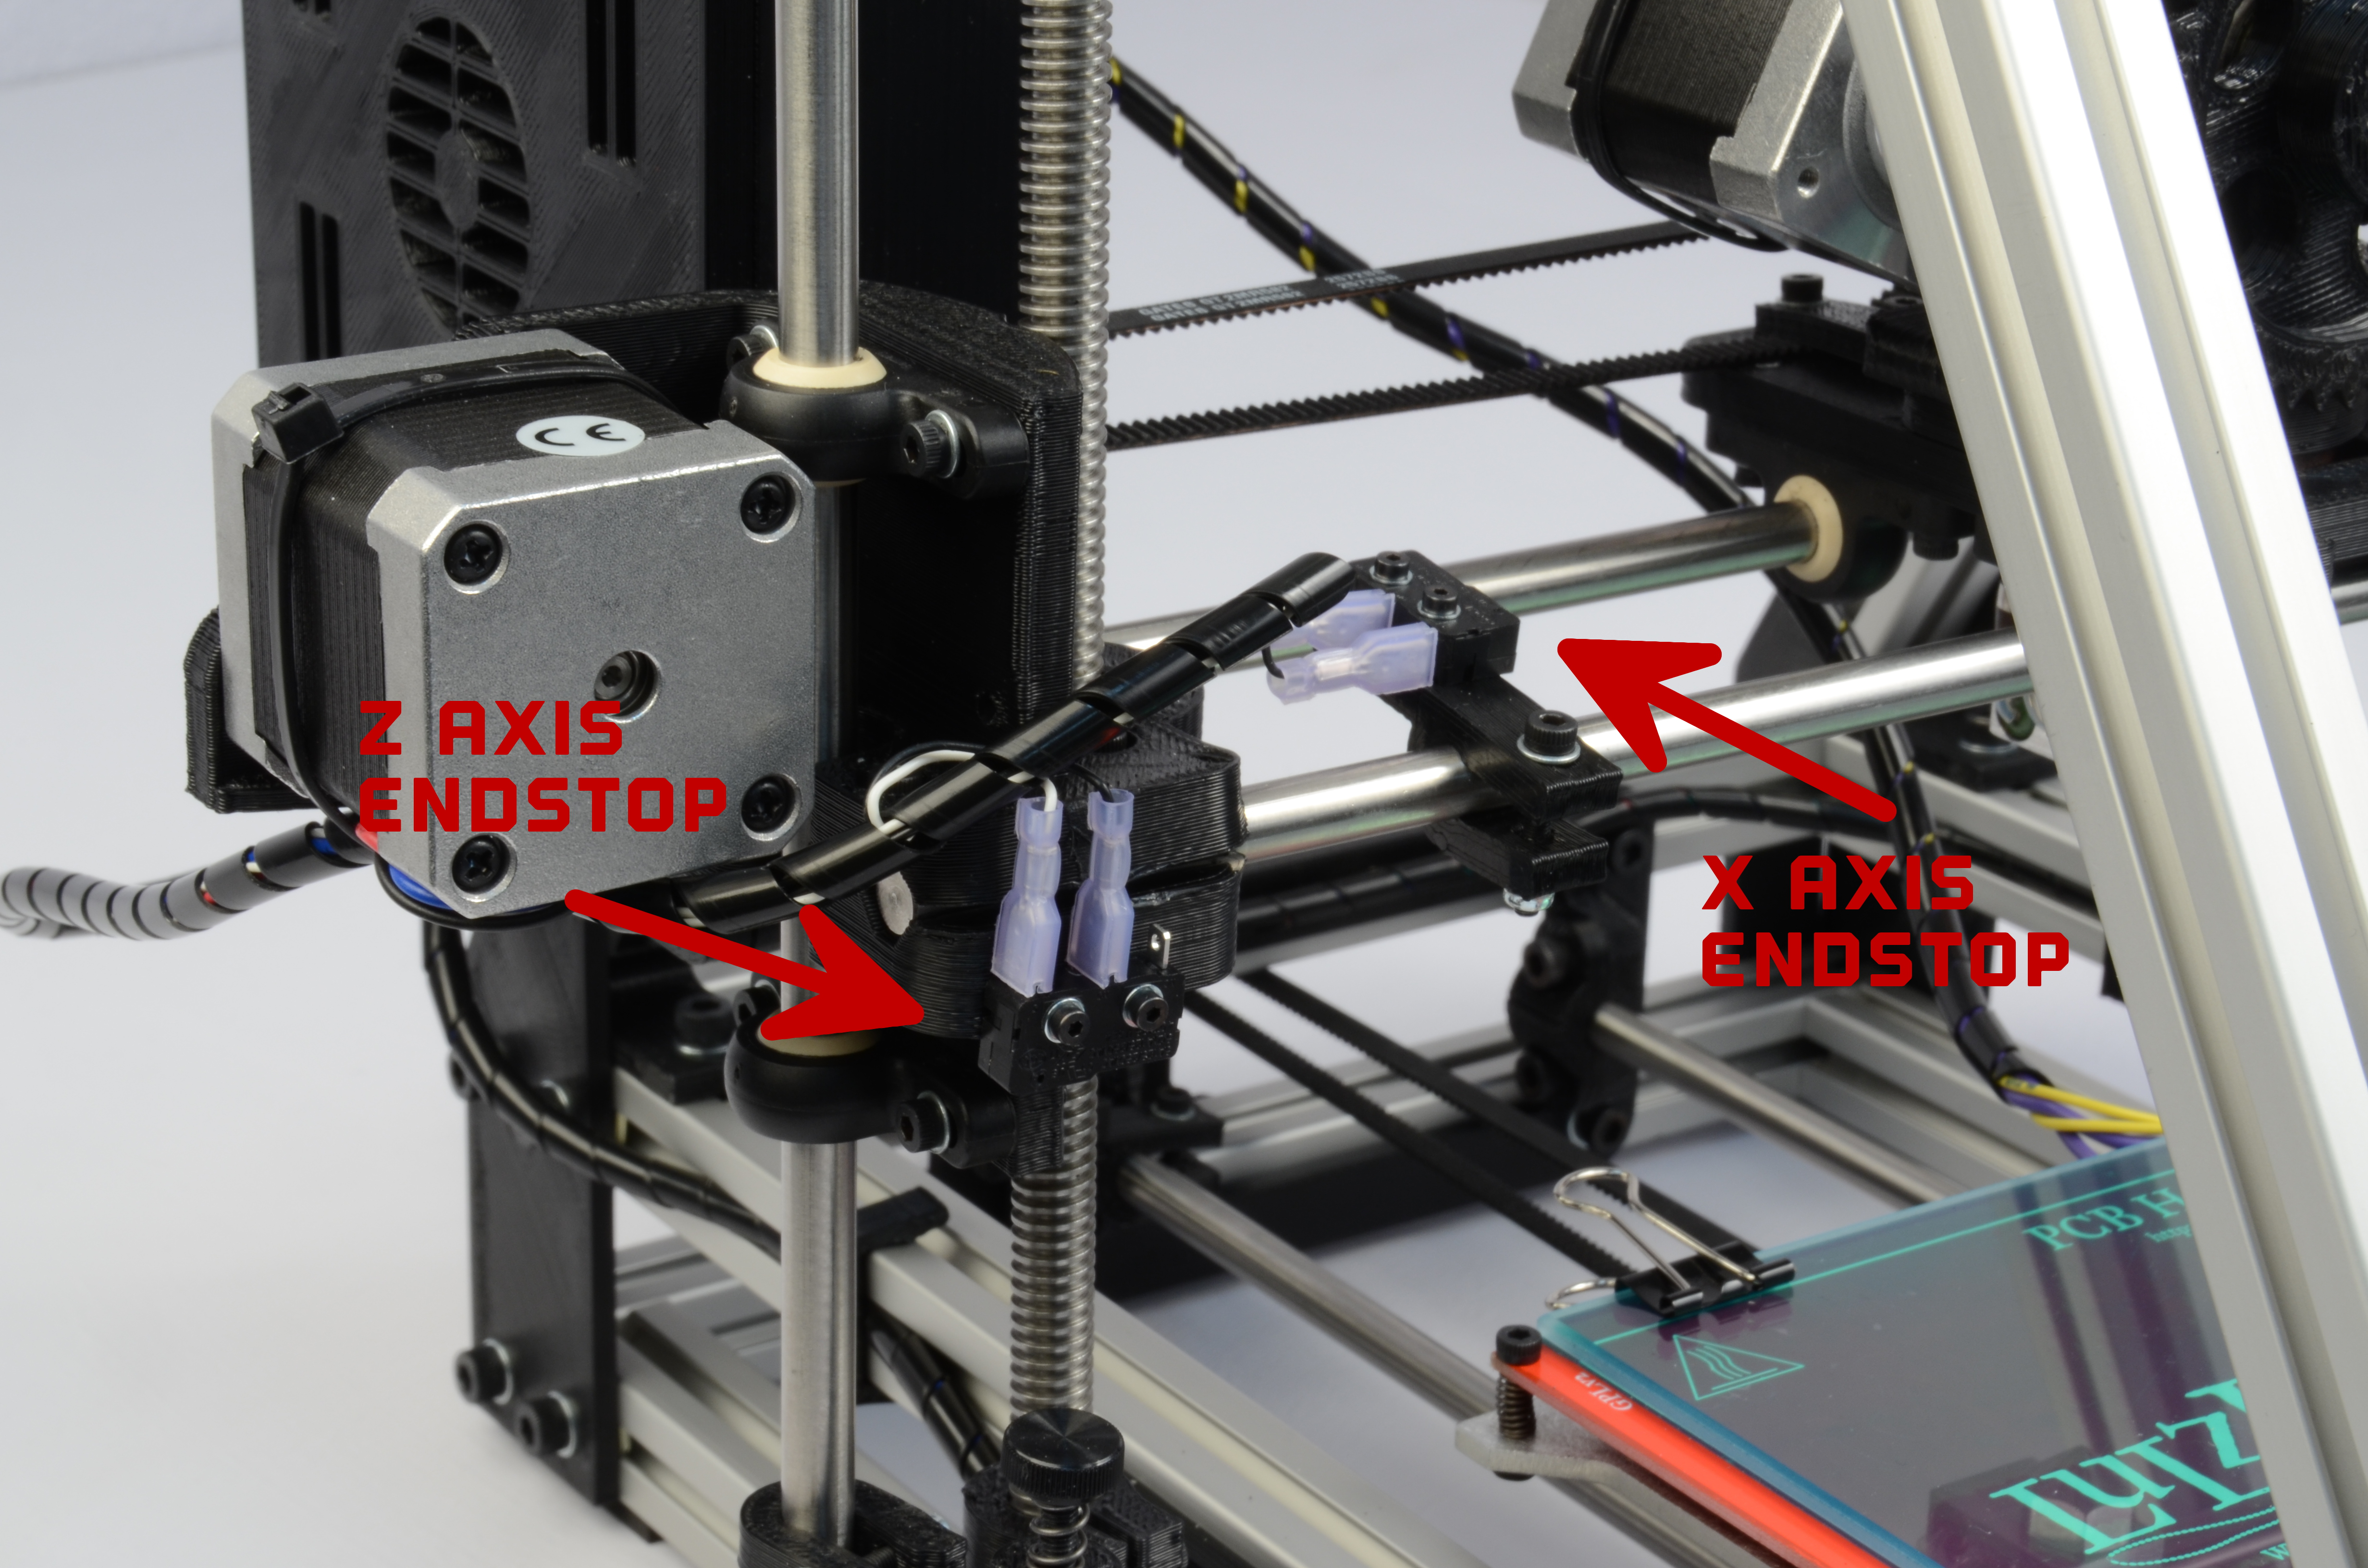
\includegraphics[keepaspectratio=true,angle=0,height=0.4\textheight,width=1.0\textwidth]{xz_endstops.jpg}
\caption{X and Z end stop locations}
\label{fig:xz_endstops}
\end{figure}
\begin{figure}[hp]
\centering
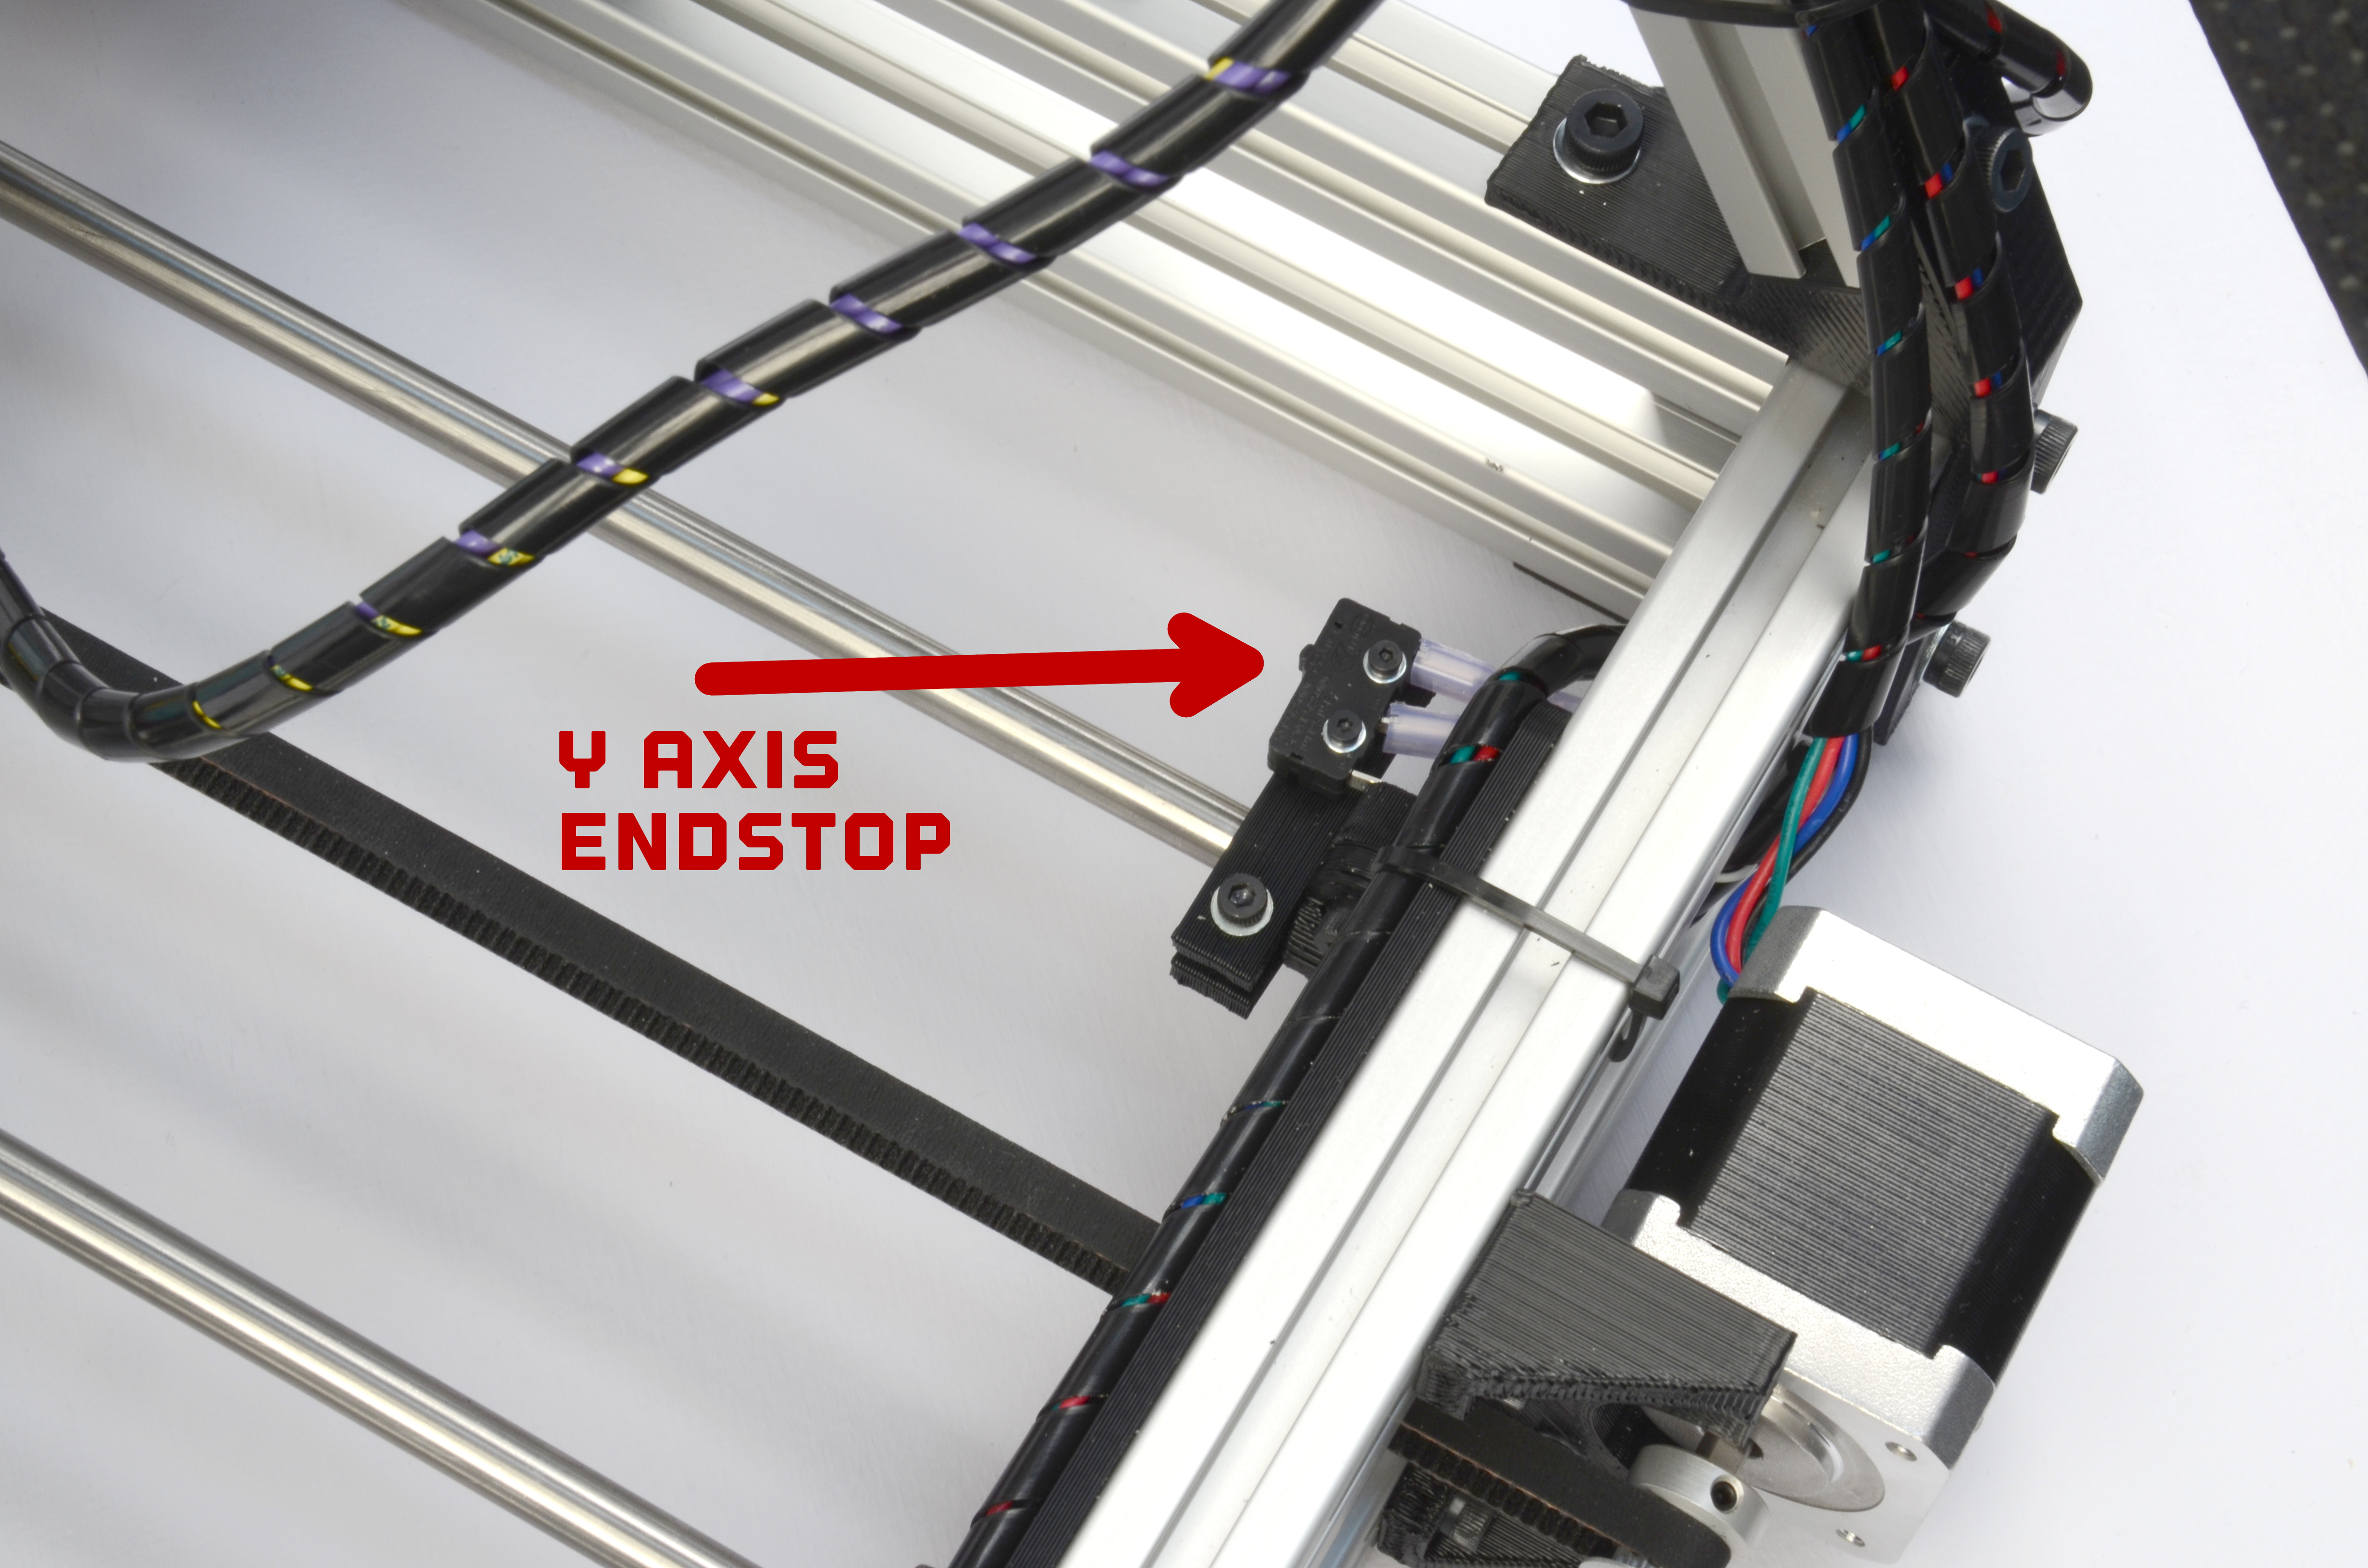
\includegraphics[keepaspectratio=true,angle=0,height=0.4\textheight,width=1.0\textwidth]{y_endstop.jpg}
\caption{Y end stop location}
\label{fig:y_endstop}
\end{figure}

\index{power supply}
\index{USB cable}
\item Unwrap the power supply and USB cable.

\textcolor{red}{MAKE SURE THE POWER SUPPLY IS COMPLETELY UNPLUGGED BEFORE MOVING ON TO THE NEXT STEP}.

\index{electronics receptacles}
\item Locate the power supply and USB receptacles along the bottom of the RAMBo electronics enclosure
(Fig. \ref{fig:electronics_plugs}, page \pageref{fig:electronics_plugs}).
\begin{figure}[hbt]
\centering
\includegraphics[keepaspectratio=true,angle=0,height=0.4\textheight,width=1.0\textwidth]{electronics_plugs.jpg}
\caption{Power supply and USB receptacles}
\label{fig:electronics_plugs}
\end{figure}
\begin{figure}[hp]
\centering
\includegraphics[keepaspectratio=true,angle=0,height=0.4\textheight,width=1.0\textwidth]{ps_plug.jpg}
\caption{Power supply plug}
\label{fig:ps_plug}
\end{figure}
\begin{figure}[hp]
\centering
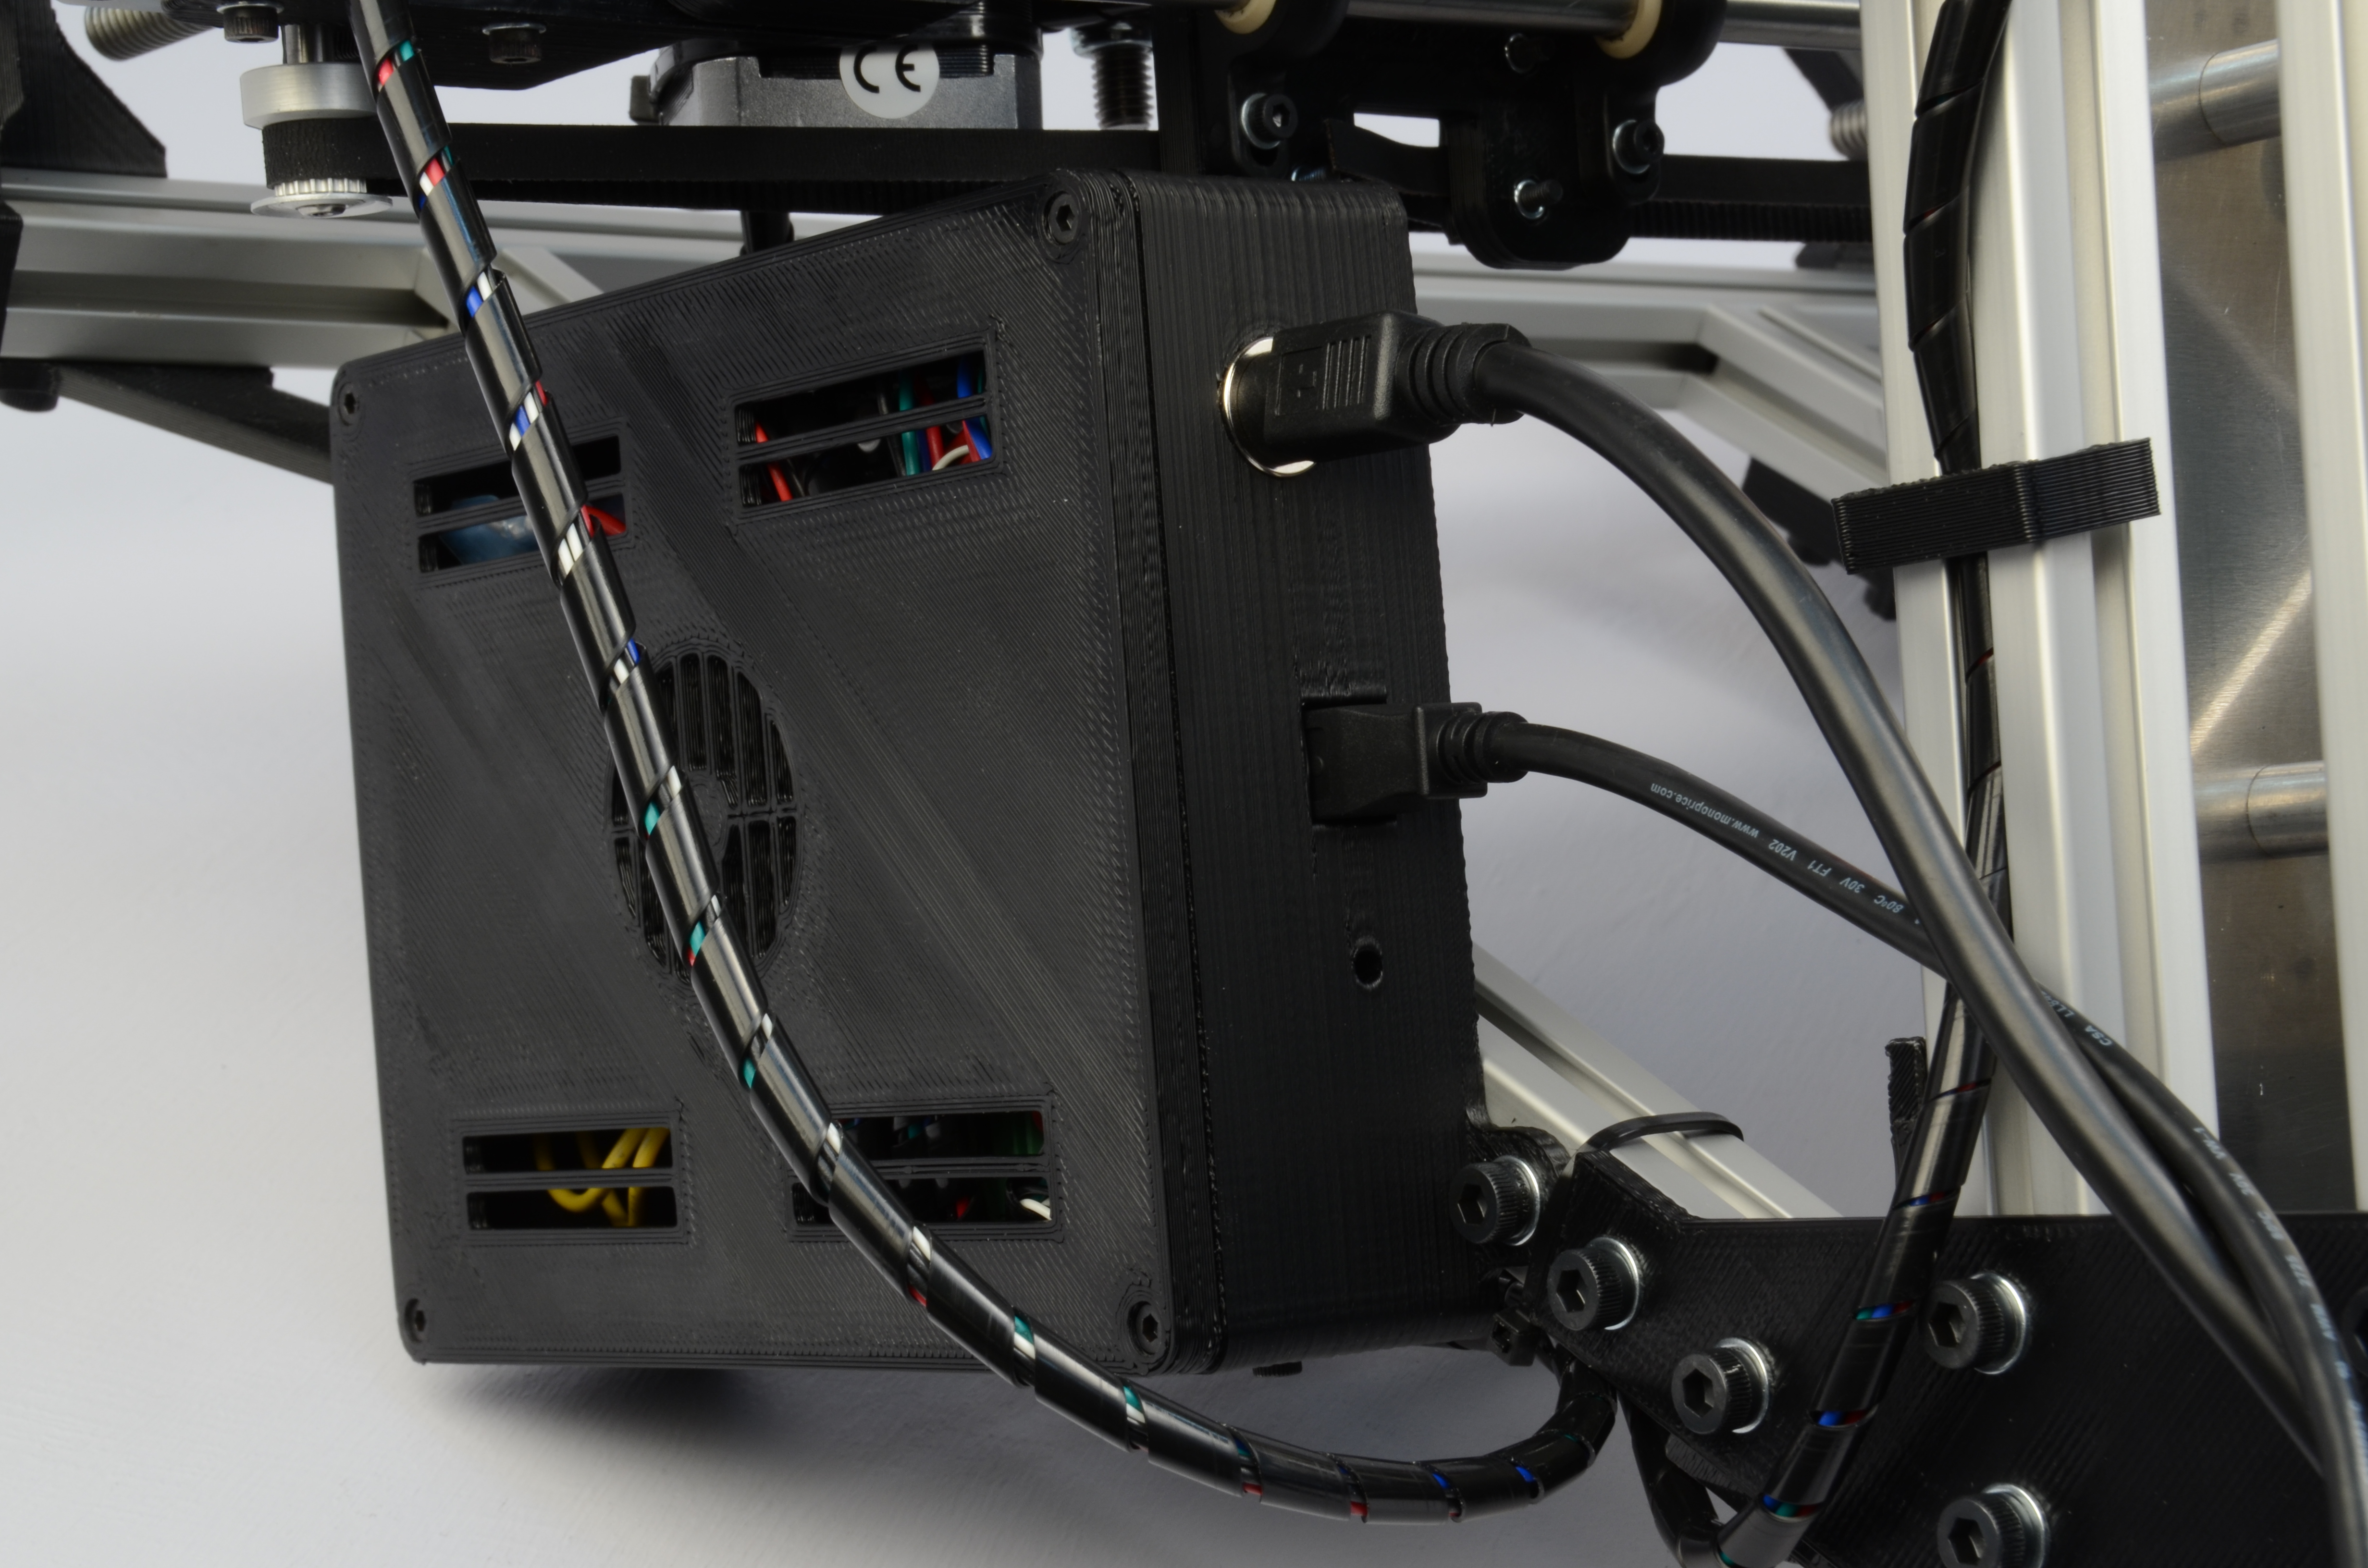
\includegraphics[keepaspectratio=true,angle=0,height=0.4\textheight,width=1.0\textwidth]{electronics_plugs_plugged-in.jpg}
\caption{The power supply and USB plugs correctly plugged in}
\label{fig:electronics_plugs_plugged-in}
\end{figure}

\index{RAMBo}
\item Plug in the USB cable, B plug (square plug) side, into the USB receptacle on the printer electronics. Plug the other end of the USB cable, A plug side, into your computer.

\index{power switch}
\item \textcolor{red}{Make sure the printer power switch is turned off} (the circle side should be depressed). The LED on the power supply should not be lit. Plug in the black power supply plug from the power supply into the power supply receptacle on the printer. The power supply plug must be aligned correctly with the flat side of the plug facing outwards from the printer. (Fig. \ref{fig:ps_plug}, page \pageref{fig:ps_plug}; Fig. \ref{fig:electronics_plugs_plugged-in}, page \pageref{fig:electronics_plugs_plugged-in}). Now you can plug in the AC power plug from the power supply into an AC power outlet.

\index{spool}
\item Locate the plastic filament spool
(Fig. \ref{fig:spool}, page \pageref{fig:spool}).
\begin{figure}[hbt]
\centering
\includegraphics[keepaspectratio=true,angle=0,height=0.4\textheight,width=1.0\textwidth]{spool.jpg}
\caption{Spool}
\label{fig:spool}
\end{figure}

\index{wrench}
\index{pliers}
\item Remove the large wing nut from the back of the spool. Take off one washer leaving the other two on the spool mounting bolt. Now locate the spool mount arm on the top right facing the rear of the printer
(Fig. \ref{fig:spool_mount}, page \pageref{fig:spool_mount}).
\begin{figure}[hbt]
\centering
\includegraphics[keepaspectratio=true,angle=0,height=0.4\textheight,width=1.0\textwidth]{spool_mount.jpg}
\caption{Spool mount}
\label{fig:spool_mount}
\end{figure}
Slide the spool mounting bolt through the hole in the spool mount arm. From the back of the spool mount arm slide the one washer on to the spool mounting bolt and turn on and snug tighten the wing nut
(Fig. \ref{fig:spool_mounted}, page \pageref{fig:spool_mounted}).
\begin{figure}[hbt]
\centering
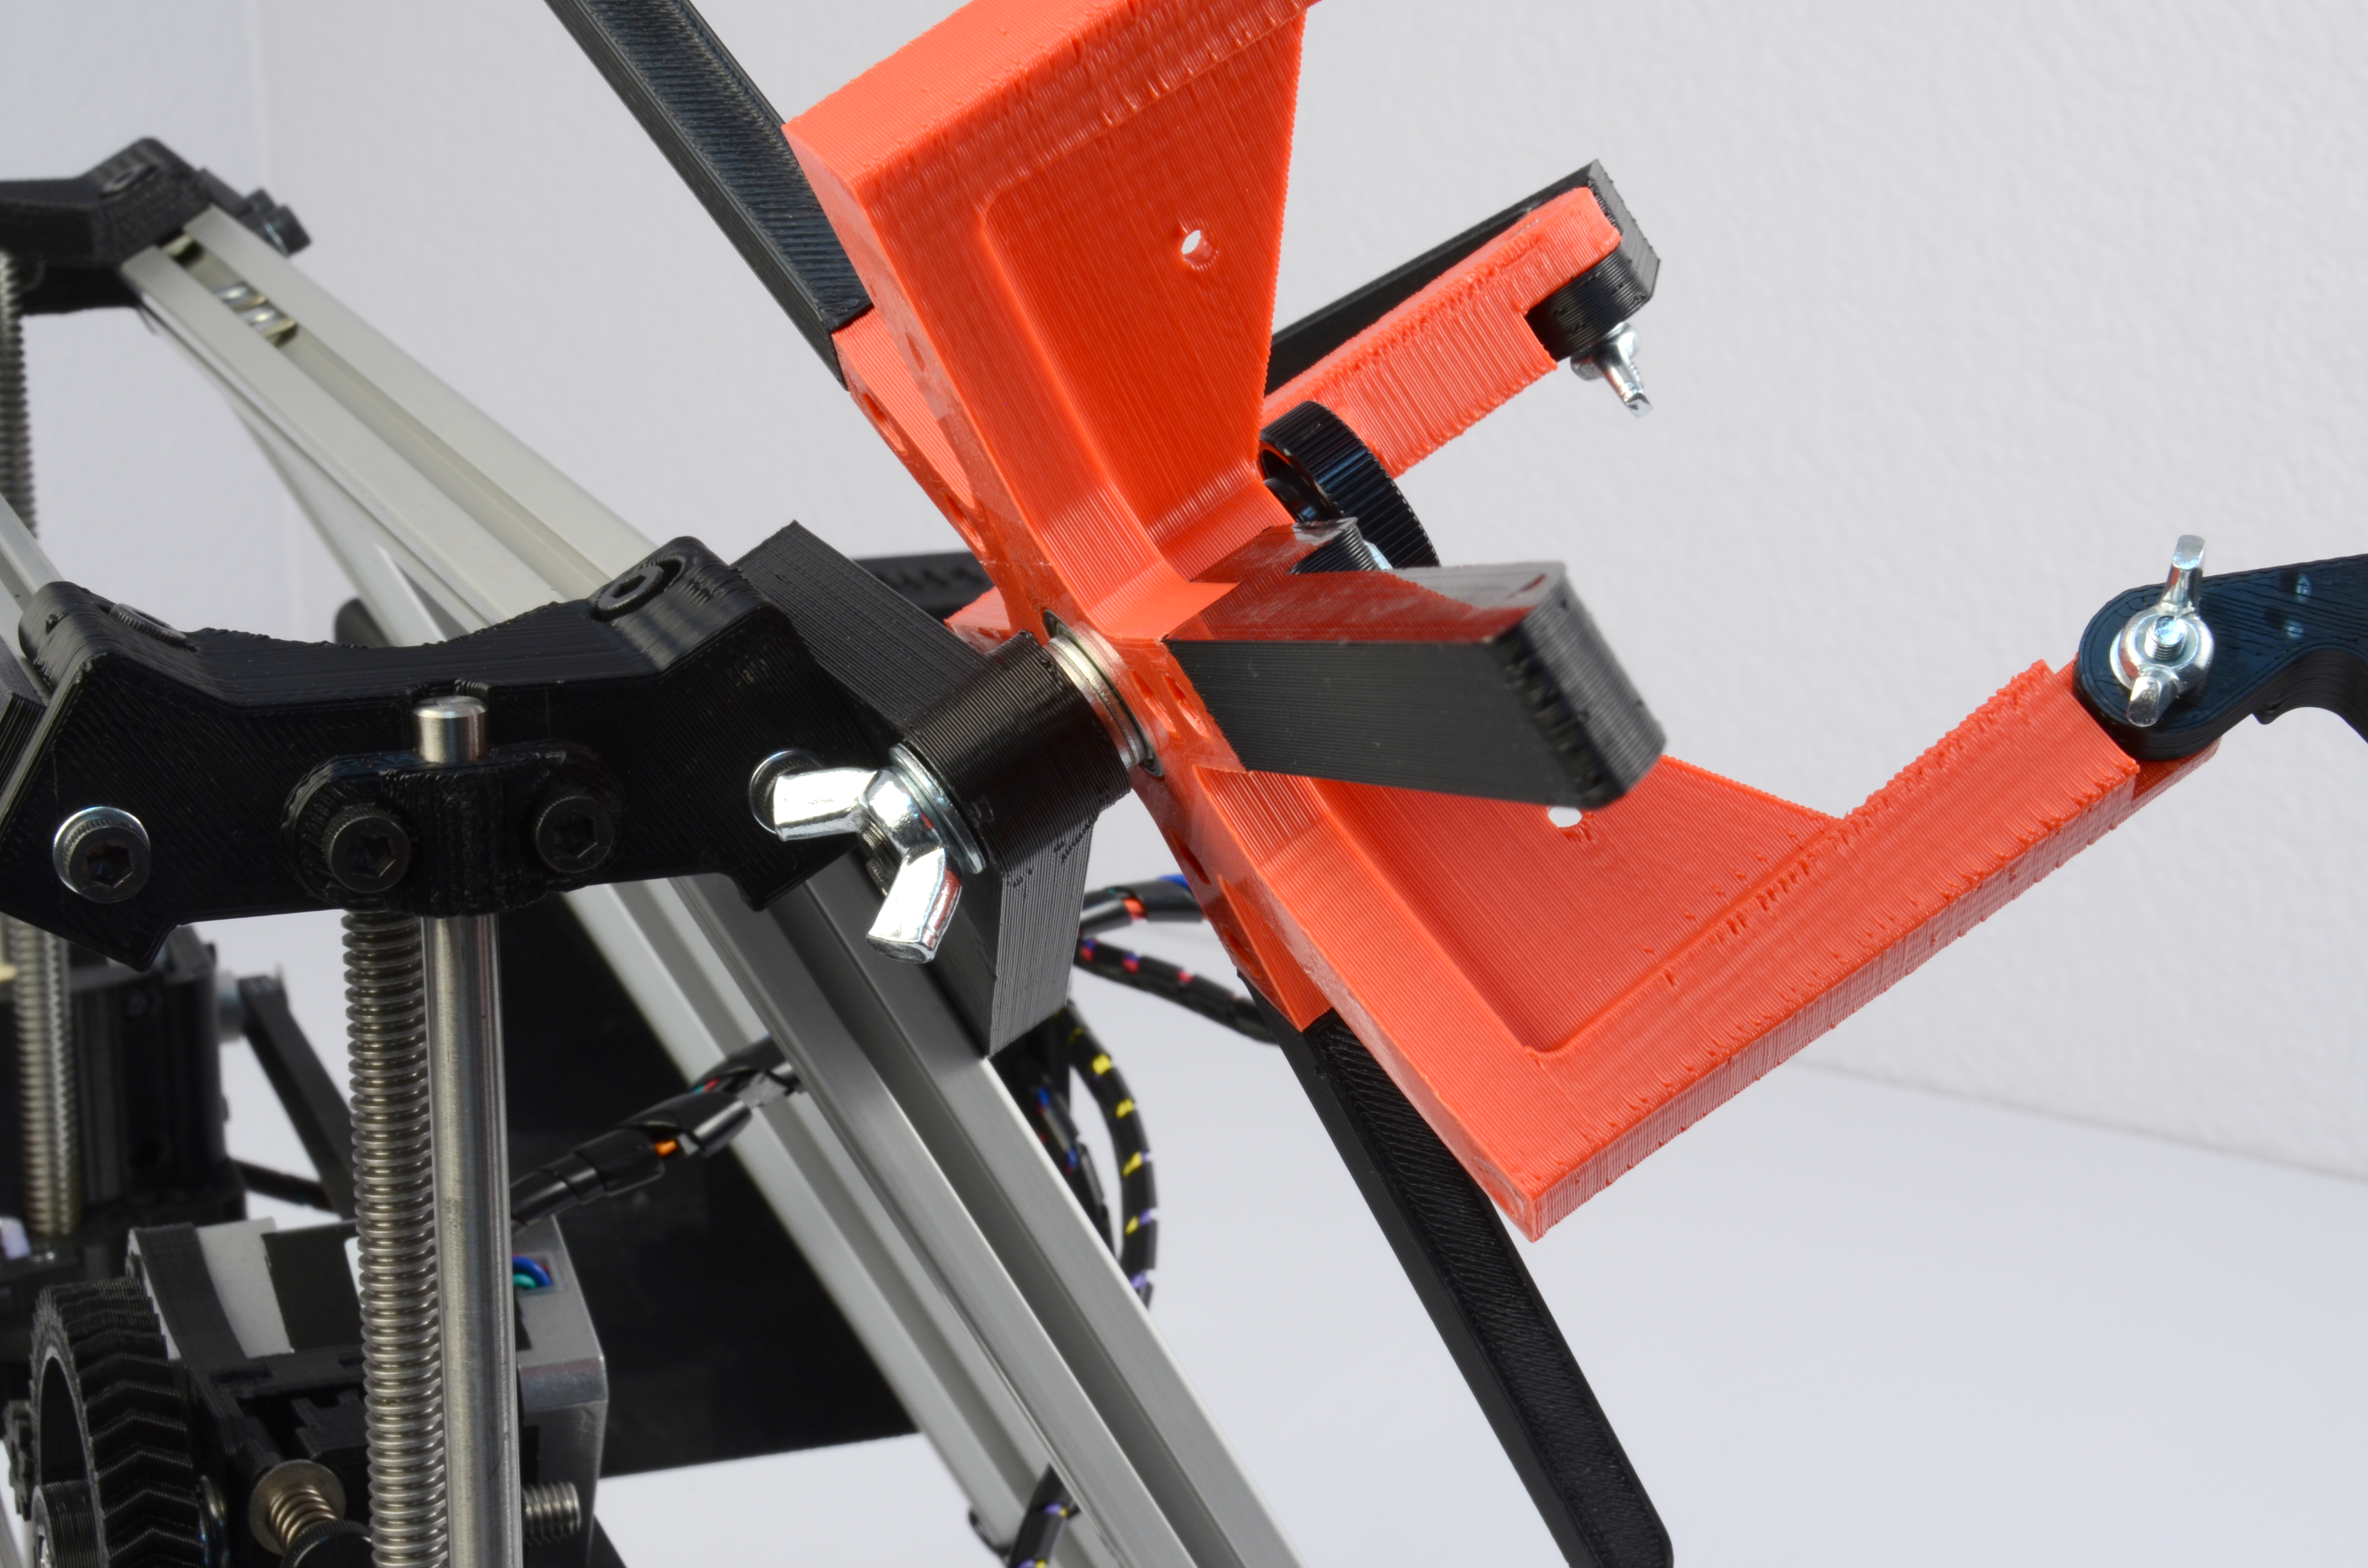
\includegraphics[keepaspectratio=true,angle=0,height=0.4\textheight,width=1.0\textwidth]{spool_mounted.jpg}
\caption{Spool mounted}
\label{fig:spool_mounted}
\end{figure}

\index{PTFE tube}
\item Locate the filament guide with attached PTFE tube
(Fig. \ref{fig:filament_guide}, page \pageref{fig:filament_guide}).
\begin{figure}[hbt]
\centering
\includegraphics[keepaspectratio=true,angle=0,height=0.4\textheight,width=1.0\textwidth]{filament_guide.jpg}
\caption{Filament Guide}
\label{fig:filament_guide}
\end{figure}

Locate the top most horizontal aluminum extrusion closest to the filament spool
(Fig. \ref{fig:filament_guide_nuts}, page \pageref{fig:filament_guide_nuts}).
\begin{figure}[hbt]
\centering
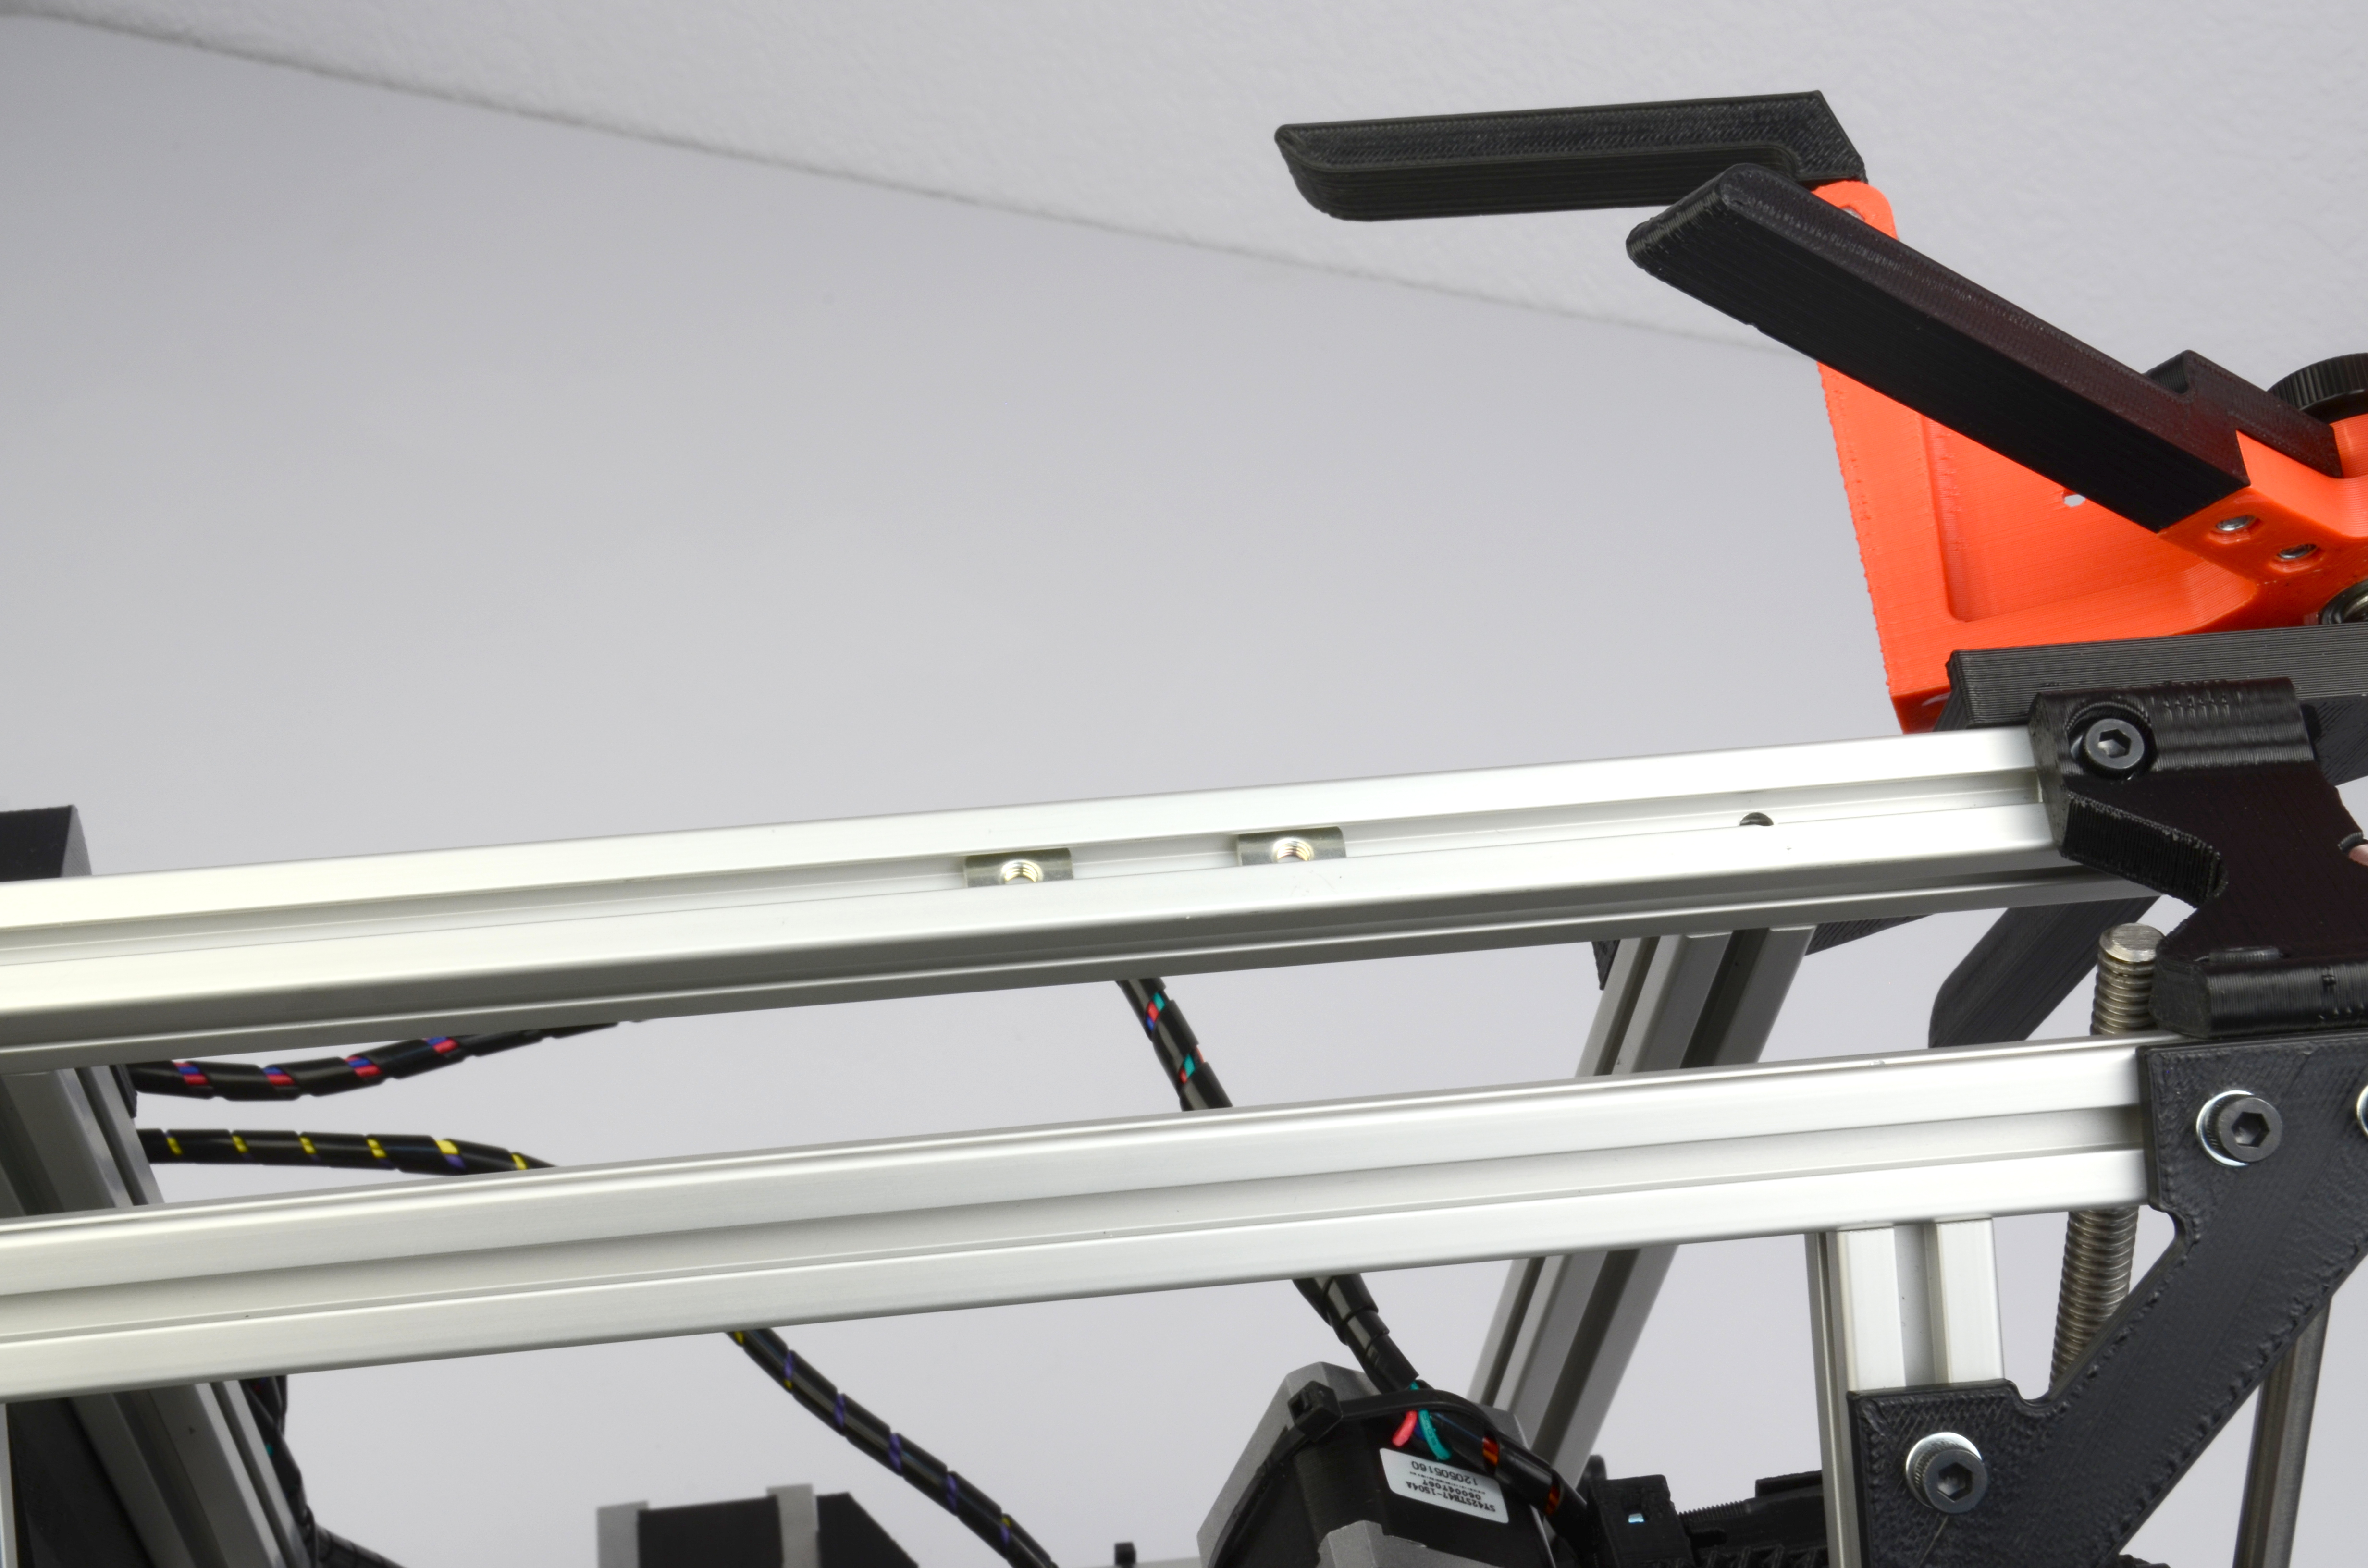
\includegraphics[keepaspectratio=true,angle=0,height=0.4\textheight,width=1.0\textwidth]{filament_guide_nuts.jpg}
\caption{Filament Guide Nuts}
\label{fig:filament_guide_nuts}
\end{figure}

In the extrusion you will find two loose t-slot nuts. The filament guide attaches to the printer by screwing in the two bolts through the filament guide into the t-slot nuts. First thread the two bolts through the filament guide into the t-slot nuts. Leave the bolts loose enough so the filament guide can slide back and forth across the extrusion. Set the filament guide 1.5-2cm away from the end of the lower arms of the filament spool
(Fig. \ref{fig:filament_guide_setting}, page \pageref{fig:filament_guide_setting}).
\begin{figure}[hbt]
\centering
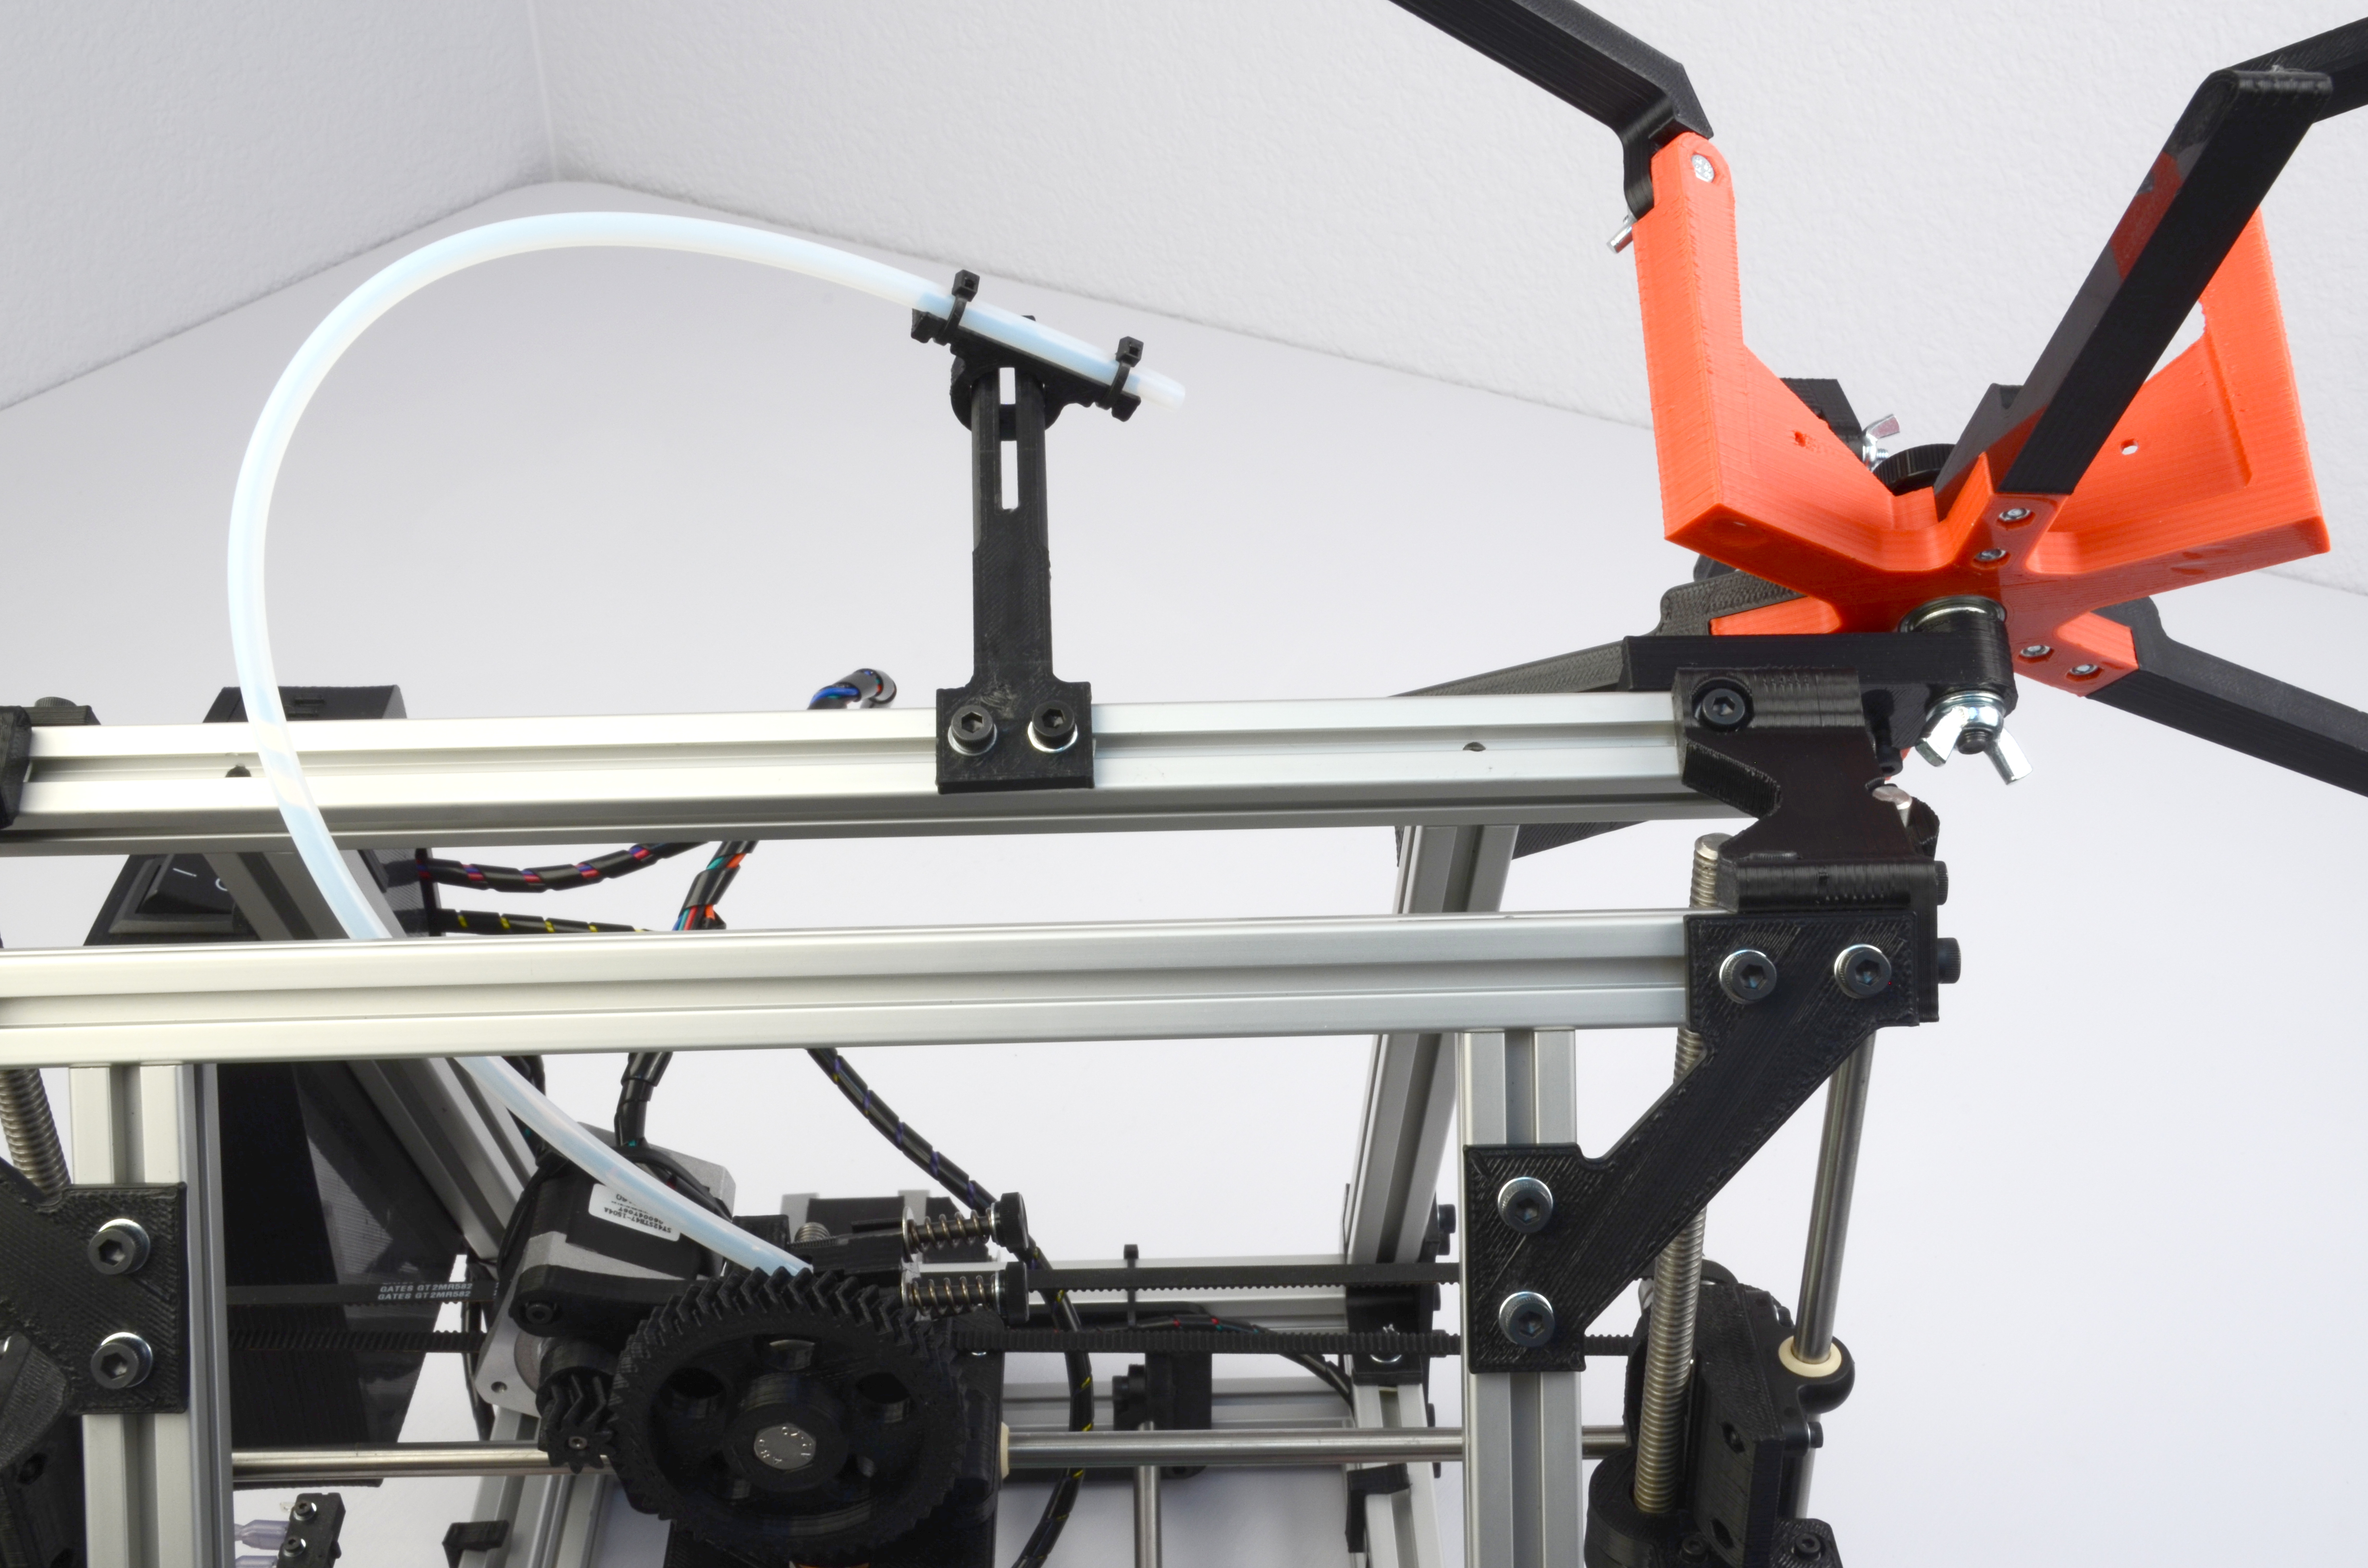
\includegraphics[keepaspectratio=true,angle=0,height=0.4\textheight,width=1.0\textwidth]{filament_guide_setting.jpg}
\caption{Filament Guide Setting}
\label{fig:filament_guide_setting}
\end{figure}
Once the filament guide is set in place, tighten down the two bolts.

\item Insert the micro SD card into the micro SD card slot, found on the top of the RAMBo electronics enclosure, shown in
Figure \ref{fig:sdramps}, page \pageref{fig:sdramps}.
\begin{figure}[hbt]
\centering
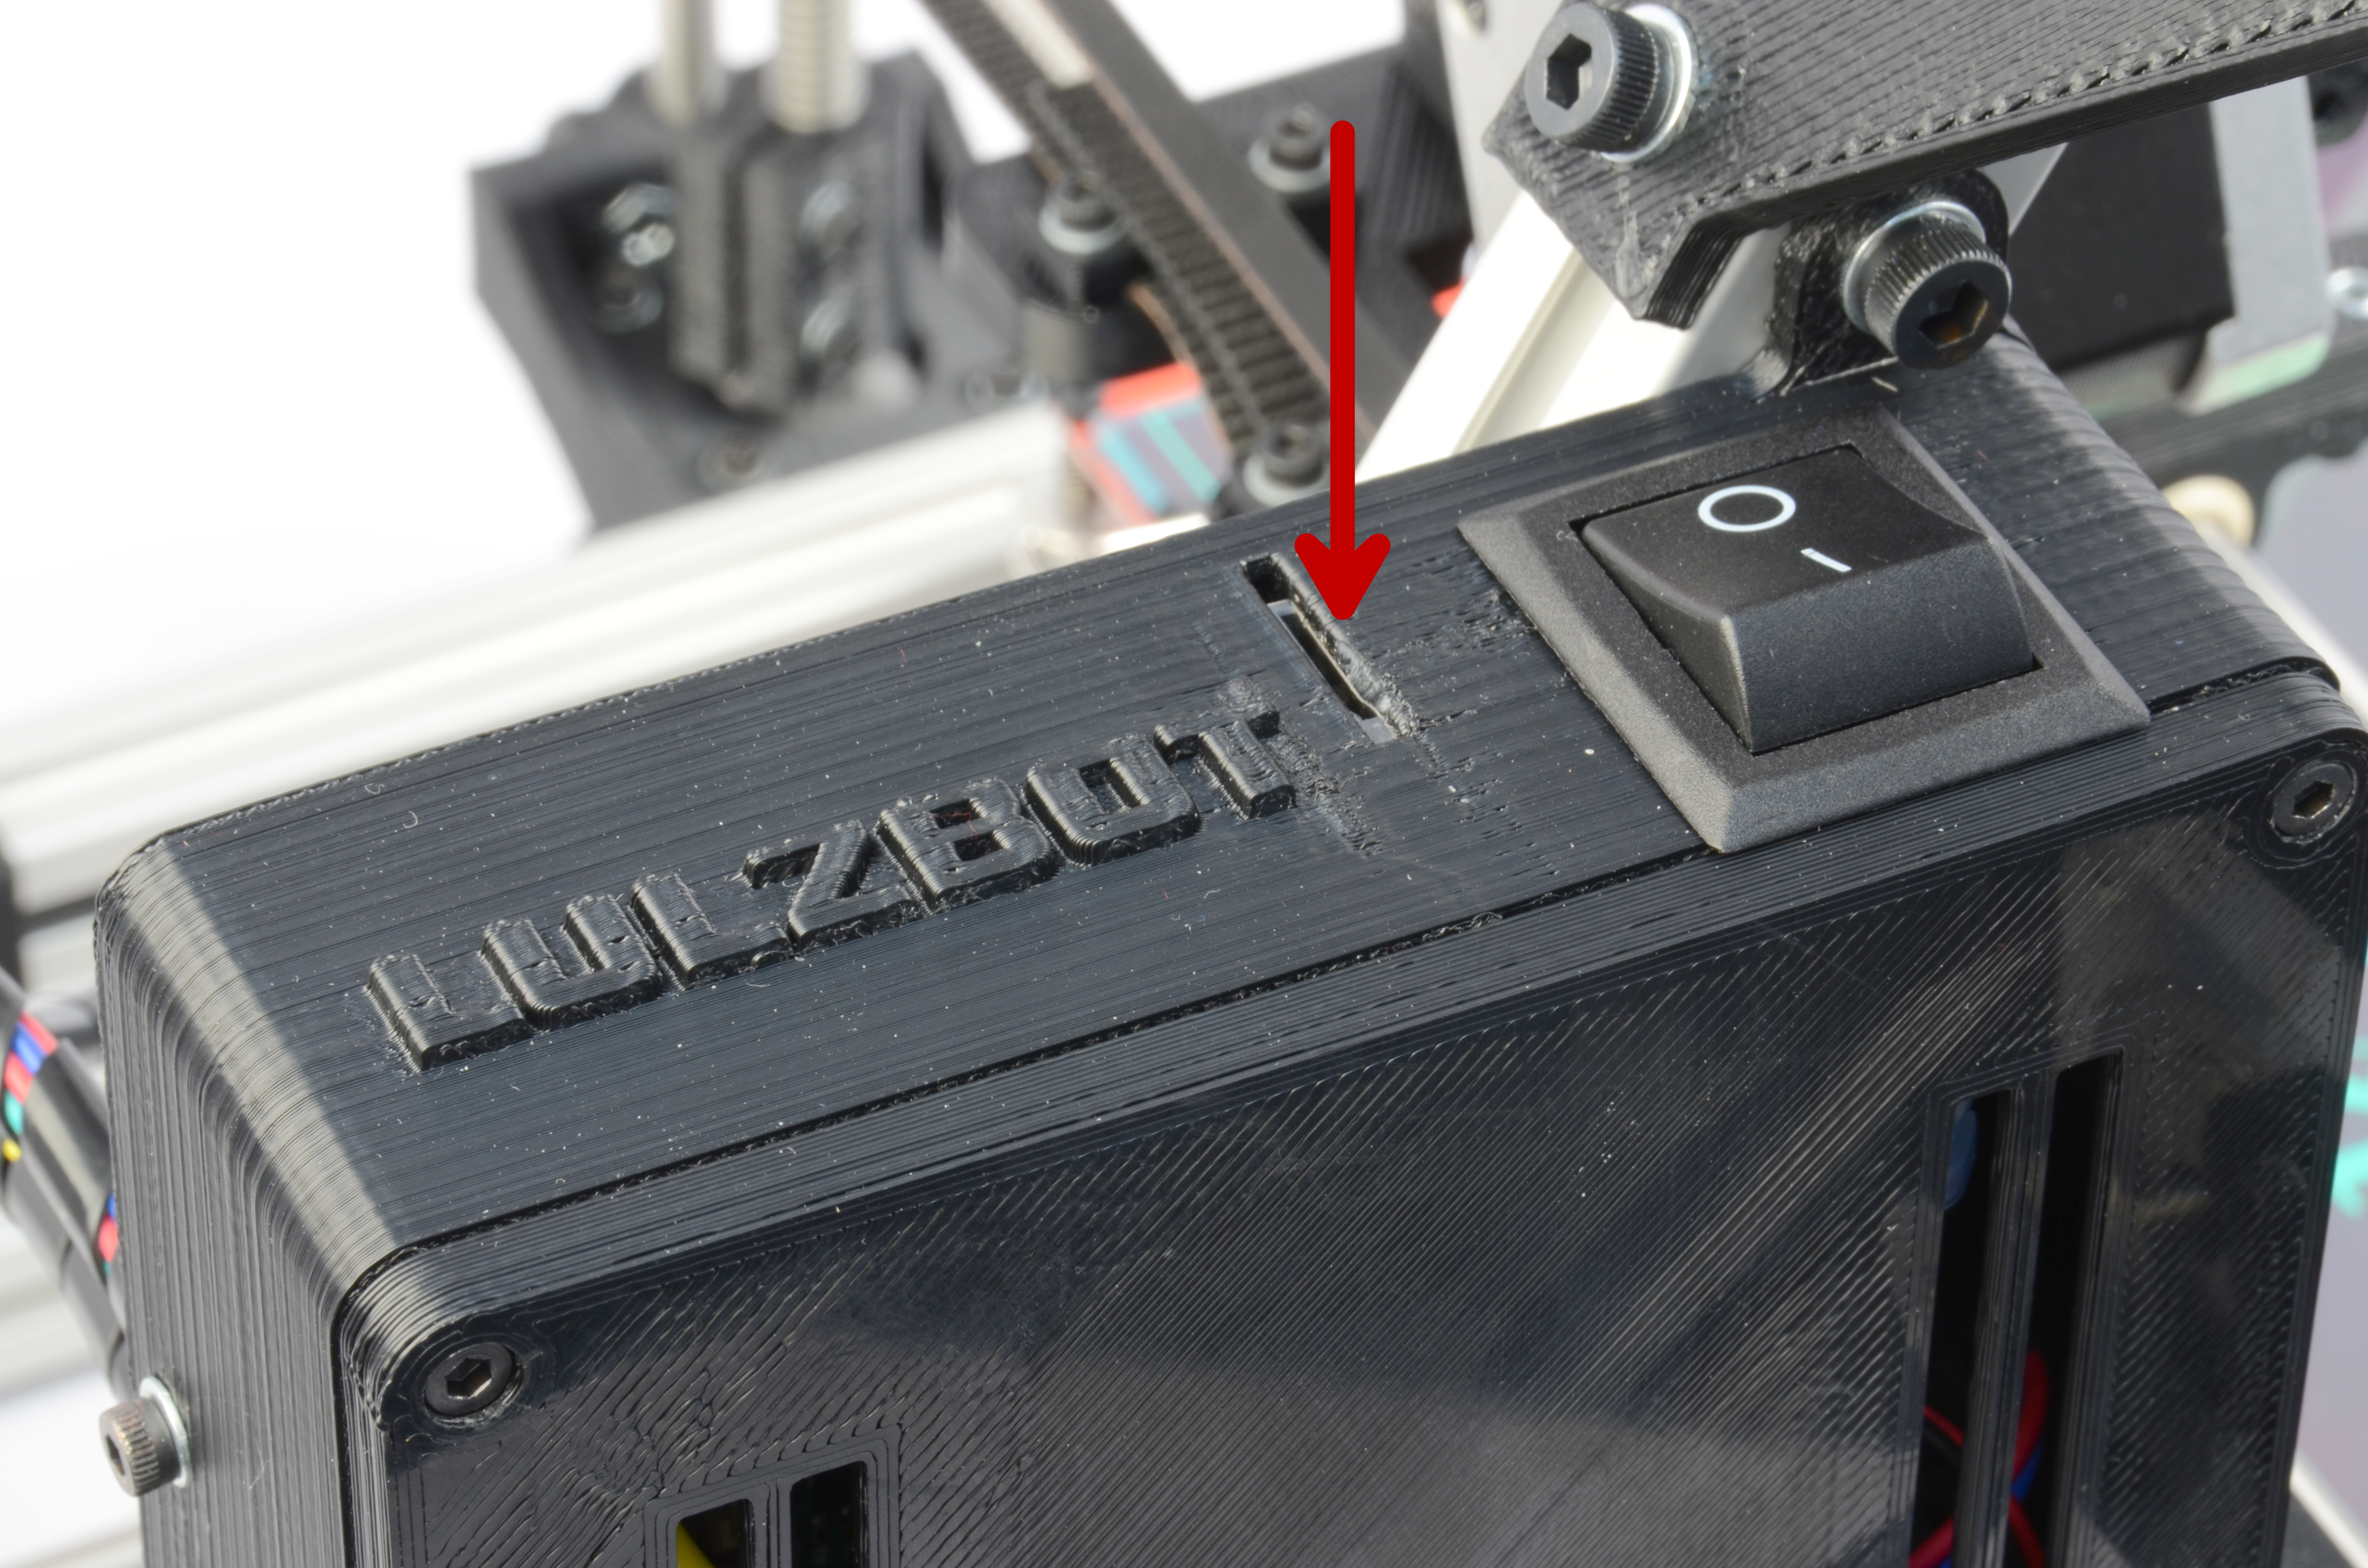
\includegraphics[keepaspectratio=true,angle=0,height=0.4\textheight,width=1.0\textwidth]{sdramps.jpg}
\caption{SDRAMPS}
\label{fig:sdramps}
\end{figure}

\end{enumerate}
}
\fi
%%% END SETUP %%%

%%% FILAMENT %%%
\iffilament
\chapter{\emph{Loading Filament}}
\thispagestyle{empty}
\markboth{Loading Filament}{LulzBot\textsuperscript{\miniscule{\texttrademark}} TAZ User Manual}
{\index{wing nuts}
\index{filament spool}
\index{spool}
\glossary{Spool}{Plastic Filament coiled and stored on a plastic reel. Preferred due to improved feeding and better mounting options.}
\glossary{Filament}{Plastic material in "string" like form, as is fed to the printer.}
\glossary{ABS}{Acrylonitrile Butadiene Styrene thermoplastic. Usually extrudes at 230C.}
\glossary{PLA}{Polylactic Acid is a corn-based biodegradable polymer. Usually extrudes at 185C.}
\glossary{HDPE}{High Density Polyethylene.}
\glossary{Polycarbonate}{A strong and impact resistant thermoplastic. Usually extrudes at ~300C.}
\glossary{HIPS}{High Impact Polystyrene.}
\glossary{Laywoo-D3}{Wooden filament similar to PLA. Contains 40 percent recycled wood. Usually prints at ~180C- 210C. Color can be changed by varying the extrusion temperature.}
\begin{figure}[hbt]
\centering
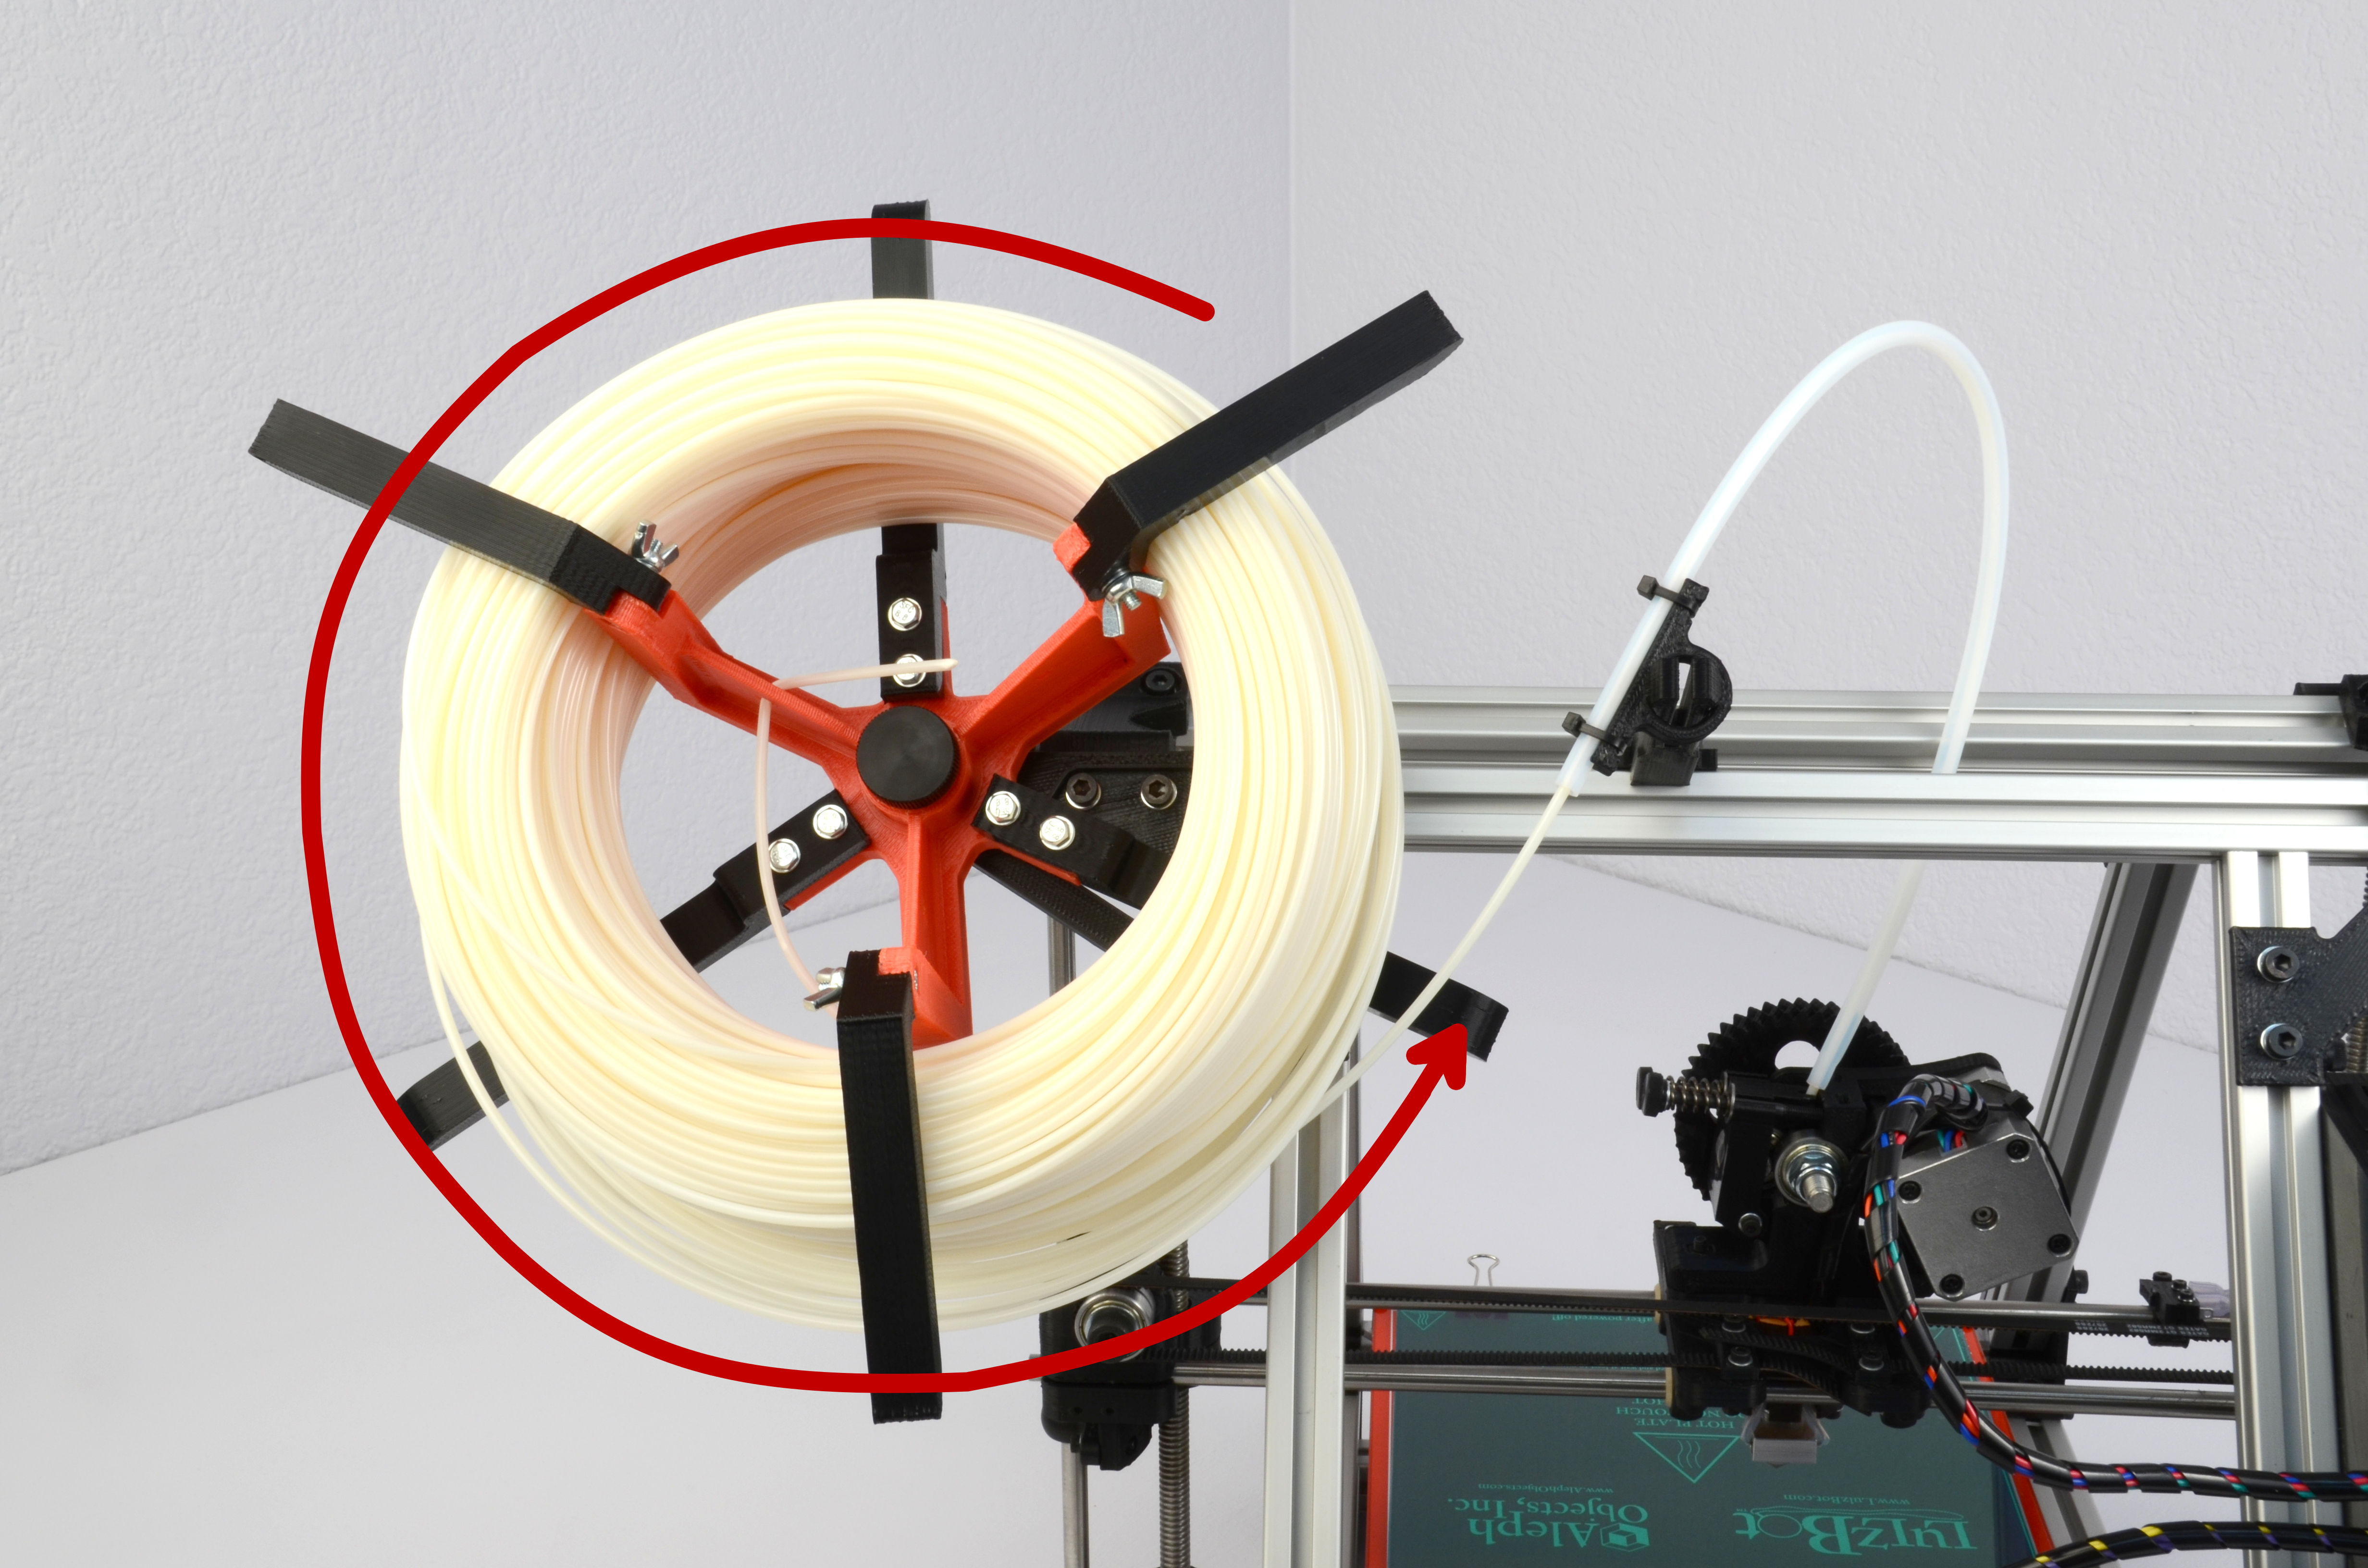
\includegraphics[keepaspectratio=true,angle=0,height=0.4\textheight,width=1.0\textwidth]{filament_spool_dir.jpg}
\caption{Filament spool direction}
\label{fig:filament_spool_dir}
\end{figure}
\begin{enumerate}
\item Loosen the three wing nuts on the upper arms of the filament spool.

\item Turn the upper arms 90 degrees upwards away from the printer.

%\glossary{Coil}{Raw filament.}

\item Remove the 5lb coil of filament from the plastic packaging, leaving the twist ties on.

\item Slide the coil over the spool upper arms. Make sure the filament coil direction is counter clock wise (from the rear of the printer) when placing the coil on to the spool
(Fig. \ref{fig:filament_spool_dir}, page \pageref{fig:filament_spool_dir}).

\item Lower the three upper arms and re-tighten the wing nuts.

\item The twist ties can now be removed. Keep the twist ties for future use if you ever need to remove the filament to change to a different filament.

\index{feed tube}
\item Feed the end of the filament through the filament feed tube.

\item If it is loose, slide the opposite end of the filament through one of the holes in hub of the filament spool. This will keep the filament from unwinding from the spool.

\end{enumerate}
}
\fi
%%% END FILAMENT %%%

%%% SOFTWARE %%%
\ifsoftware
\chapter{\emph{3D Printer Software}}
\thispagestyle{empty}
\markboth{3D Printer Software}{LulzBot\textsuperscript{\miniscule{\texttrademark}} TAZ User Manual}
{\section{Software Overview}
\index{software}
Aleph Objects, Inc., the maker of the LulzBot TAZ completely supports free/libre hardware and software. Along with the TAZ being a free/libre hardware design, it has been tested to work with 100\% free/libre software.

To operate your desktop 3D printer you will need to install a few software packages onto your PC. You will need a 3D printer host, an \texttt{.STL} to \texttt{.gcode} generator, and optional CAD or 3D modeling software.

\index{GNU/Linux}
\index{Macintosh}
\index{Windows}
\index{operating system}
All of the following free/libre software is available for GNU/Linux, Windows, and Macintosh. However, we highly recommend using these softwares on GNU/Linux.

\index{download}
The required software can be found in the Support/Downloads section at \texttt{www.LulzBot.com}. You will also find instructions there for installing each program onto your PC. Make sure to select the software version that corresponds with the TAZ 3D printer and the operating system you are using.

\section{Slic3r}
\index{gcode}
\index{STL}
\index{CAD}
\index{resolution}
\index{Slic3r}
Website: \texttt{www.slic3r.org}

The Slic3r software is the first tool in the chain of 3D printing software
(Fig. \ref{fig:slic3r}, page \pageref{fig:slic3r}).
\begin{figure}[hbt]
\centering
\includegraphics[keepaspectratio=true,angle=0,height=0.4\textheight,width=1.0\textwidth]{slic3r.png}
\caption{Slic3r application, STL to Gcode generator}
\label{fig:slic3r}
\end{figure}

Slic3r uses commonly used \texttt{.STL} (stereolithography) files to create \texttt{.gcode} files. Gcode files contain instructions for the 3D printer on where, when, and how fast to make movements. However, Gcode programming is not very suitable for CAD and 3D design. This is where Slic3r and the \texttt{.STL} file comes into use. The \texttt{.STL} file is a 3D model file that can be exported by all common CAD and 3D modeling software. The Slic3r software then slices the \texttt{.STL} 3D model into layers and print paths to create a 3D printable \texttt{.gcode} file.

To launch Slic3r navigate to the \texttt{Slic3r} directory and launch the \texttt{slic3r.pl} file. On GNU/Linux operating systems you may need to set the \texttt{slic3r.pl} file as executable. On other operating systems it may be called \texttt{slic3r.exe}.

\index{download}
Slic3r includes very simple settings that allow you to easily refine prints. You can create multiple configurations for changing printer setups including nozzle sizes and desired print resolution. For ease of use we have pre-defined Slic3r configurations available in the Support/Downloads section at \texttt{www.LulzBot.com}. Download the configurations to your \texttt{Slic3r} directory.

\index{configuration}
\subsection{Loading Configurations}
To load configurations press the \texttt{Load Config...} button. In the file browser that opens, locate the downloaded configuration files. Select the configuration file that matches the nozzle size currently installed on the printer (0.5mm nozzle is installed by default). Press \texttt{Open} and the pre-defined configuration will load into Slic3r. You can also save custom configurations for yourself by pressing the \texttt{Export Config...} button. A file browser will open that allows you to define a name and save your custom configuration. 

\index{STL}
\index{plater}
\subsection{Loading STL files}
To load an \texttt{.STL} 3D model file into Slic3r, activate the Plater tab and click the \texttt{Add...} button. In the file browser navigate to the \texttt{.STL} you wish to load and click \texttt{Open}. The silhouette of the model will appear in the Plater diagram. To print more than one copy of the model at a time select the model name from the list and click the \texttt{More} button. With each press of the \texttt{More} button an additional copy of the model will be added to Plater. To remove a copy of the model select the model name again and click \texttt{Less}. To completely remove the model from Plater select the model name and click \texttt{Delete}.

\index{gcode}
\subsection{Export Gcode files}
Once you have finished setting your part(s) in Plater you can generate the Gcode by clicking \texttt{Export G-Code...}. In the file browser navigate to where you would like to save the \texttt{.gcode} file and list a name to save the file as. Click \texttt{Save} and Slic3r will begin generating the \texttt{.gcode} file. When Slicer is finished you will receive a prompt. If you have created a plate with multiple model designs you can also use the \texttt{Export STL...} function to save an \texttt{.STL} file for quickly reproducing the same plate of models.

\section{Printrun}
%%% XXX shouldn't have to do it this way.
%%% HOWTO get page number from section? Ala  sec:Printrun
\label{Printrun}
\index{extruder}
\index{extrusion}
\index{temperature}
\index{gcode}
\index{SD card}
\index{Printrun}
Website: \texttt{github.com/kliment/Printrun}

The host software, Printrun, is used to start up and control your 3D printer 
(Fig. \ref{fig:printrun}, page \pageref{fig:printrun}).
\begin{figure}[hbt]
\centering
\includegraphics[keepaspectratio=true,angle=0,height=0.4\textheight,width=1.0\textwidth]{printrun.png}
\caption{Printrun application for 3D printer control}
\label{fig:printrun}
\end{figure}
The host controls include: setting the extruder and print surface temperatures, manual control of each axis, and manual extrusion. The host is also where you will push print files (\texttt{.gcode}) to the 3D printer or load print files from the SD card for printing out model designs.

\index{pronterface}
\index{GNU/Linux}
To launch Printrun, navigate to the \texttt{Printrun} directory and launch the \texttt{pronterface.py} file. On GNU/Linux operating systems you may need to set the \texttt{pronterface.py} file as executable. On other operating systems the file may be called \texttt{pronterface.exe}.

\subsection{Connecting the Printer}
\index{connecting}
\index{Printrun}
\index{USB cable}
\index{port}
\index{baud rate}
To start up the printer, first you will need to connect to the printer with Printrun. Make sure you have connected the USB cable from your PC to the printer before launching Printrun. If not, close Printrun, connect the USB cable, and relaunch Printrun. In the top left \texttt{Port} pull down menu select the correct port for the printer (generally \texttt{/dev/ACM0}). On other operating systems the port may be named such as \texttt{COM1} or \texttt{tty.usbserial-USB-ID}. If you only have one printer connected there will only be one port available to select. Make sure the port baud rate is set to \texttt{115200} in the pull down menu to the right of the port selection. You can refresh the USB ports, by clicking the \texttt{Port} button.

Now, to connect to the printer click the \texttt{Connect} button. In the text output window you will see multiple return lines. If you see \texttt{Printer is now online} you have succesfully connected to the printer. The printer control buttons on the left will also darken and become clickable after connecting. When you need to disconnect the printer simply press the \texttt{Disconnect} button.

\subsection{Printer Controls}
\index{Printrun}
\index{hot end}
All of the printer controls can be found on the left side of the Printrun interface
(Fig. \ref{fig:printrun_controls}, page \pageref{fig:printrun_controls}).
\begin{figure}[hbt]
\centering
\includegraphics[keepaspectratio=true,angle=0,height=0.4\textheight,width=1.0\textwidth]{printrun_controls.png}
\caption{Printrun controls}
\label{fig:printrun_controls}
\end{figure}
To set the hot end and print surface temperature first click the \texttt{Monitor Printer} check box on. This will enable the printer temparature bars and graph. The hot end and print surface controls are labeled \texttt{Heater} and \texttt{Bed}. Select the temperature setting by using the pull down menu for pre-defined temperature settings. You can also set custom temperature settings by typing into the temperature box.

\index{temperature}
To turn on the hot end and/or printer surface click the respective \texttt{Set} button. The \texttt{Set} button will highlight orange when the temperature is set to on for that component. When the hot end or print surface is set to on you will see the temperature bar and graph display the set temperature and the current temperature. When both components have reached the correct temperature, the printer is ready for printing. Clicking the \texttt{Off} button will turn off that component and highlight the \texttt{Off} button blue.

\index{extrude}
\index{hot end}
Below the temperature controls are the manual extrusion controls. There you can manually extrude plastic through the hot end and retract the plastic filament from the hot end. The \texttt{Extrude} button will feed the amount of plastic, set to the right in mm, through the hot end. The rate at which the plastic is fed is set below the extrusion length (mm/min). The \texttt{Reverse} button will perform the opposite of \texttt{Extrude}, pulling the plastic filament back out of the hot end.

\index{manual controls}
\index{axes}
\index{X axis}
\index{Y axis}
\index{Z axis}
The large pattern of buttons above the temperature controls are the axes manual controls. These functions allows you to manually move each of the three axes of the printer. The circular pattern of four quadrants controls the X and Y axes. The top and bottom quadrants move the Y axis; the top in the positive direction (forward) and the bottom in the negative direction (back). The left and right quadrants move the X axis; the left in the negative direction (left) and the right in the positive direction (right).

Each quadrant is split into four sections that control the length of movement of 0.1mm, 1mm, 10mm, or 100mm. The innermost section moves the axis 0.1mm with each section outwards a larger movement with the outside section moving the axis 100mm.

The linear control bar to the right controls the Z axis. The Z axis is also seperated into multiple movement lengths; 0.1mm, 1mm, and 10mm. The upper three buttons move the Z axis up and away from the printer surface; the three lower buttons move the Z axis closer to the print surface.

\index{home}
The four triangular buttons around the circular pattern are the axes home buttons. Each home button will move that axis in the negative direction until the end stop is activated. There is a home button for the X, Y, and Z axes. There is also a white home all button that homes all of the axes at once.

\index{motors}
The \texttt{Motors off} button will deactivate all motors allowing all of the axes to be moved by hand.

\index{end stops}
Caution: when homing, the axis will continue to move in the negative direction until the end stop switch is activated. If the printer is ever transported make sure the end stop switches are in the correct position before printing. The end stops should be aligned so they will be activated by the axes. If an axis has missed an end stop and is continuing to try to move in the negative direction, immediately turn the power switch to the off position. If a print file was running pause the print by clicking the \texttt{Pause} button. Realign the end stop and try homing again.

\subsection{Loading Print Files}
\index{load files}
\index{gcode}
\index{Printrun}

To load a \texttt{.gcode} file into Printrun click the \texttt{Load file} button. Navigate to the \texttt{.gcode} file in the file browser and click \texttt{Open}. You will now see a 2D images of the first layer of your model design in the Gcode viewer
(Fig. \ref{fig:printrun_viewer}, page \pageref{fig:printrun_viewer}).
\begin{figure}[hbt]
\centering
\includegraphics[keepaspectratio=true,angle=0,height=0.4\textheight,width=1.0\textwidth]{printrun_viewer.png}
\caption{Printrun viewer}
\label{fig:printrun_viewer}
\end{figure}
Click the Gcode viewer window to see a more detailed version of the sliced model. In the pop-up Gcode viewer you can zoom in using the mouse scroll wheel and flip through layers with the up and down arrow keys. The lines shown in the Gcode viewer represent the path the extrusion nozzle will follow to print the model.

For more information on using Printrun see the Printrun page in the Support/Downloads section at \texttt{www.LulzBot.com}. Instructions for running a print can be found in the
%%% XXX Tag this
Starting the First Print section in this manual.

\section{CAD and 3D Modeling Software}
\index{CAD}
\index{software}
\index{STL}

Currently LulzBot is not distributing a CAD or 3D modeling software package. However, there are multiple free/libre software packages available. Other common non-free CAD and 3D modeling software are also capable of exporting the required \texttt{.STL} files.

On some CAD and 3D modeling software you will need to select millimeters as the output unit. If possible it is best to build your 3D design in metric units rather than emperial units. Slic3r requires .STL files sized in millimeters. If an .STL with inches as units is loaded into the Slic3r, the model will be scaled much smaller than expected. The software listed below outputs millimeters as the unit by default.

\subsection{FreeCAD}
\index{FreeCAD}
\index{GNU/Linux}
\index{Windows}
\index{Macintosh}
Website: free-cad.sourceforge.net

Although still in development, FreeCAD is a great free/libre CAD application. Containing a full GUI for building CAD models, FreeCAD is capable of creating simple to complex designs. STL files can also easily be exported for use with 3D printing. FreeCAD is available for GNU/Linux, Windows, and Mac. The latest development version is recommended.

\subsection{OpenSCAD}
\index{OpenSCAD}
\index{GNU/Linux}
\index{Windows}
\index{Macintosh}
Website: openscad.org

OpenSCAD is another free/libre CAD software; however, different than FreeCAD, it is script based. Rather than using a GUI to generate CAD designs, OpenSCAD CAD designs are created using script based renderings. Users with programming experience would find this very useful. Also, OpenSCAD uses a simple script language that is easy to learn for users with little or no programming experience.

\subsection{Blender}
\index{Blender}
\index{GNU/Linux}
\index{Windows}
\index{Macintosh}
Website: blender.org

The most widely used Free/Libre 3D modeling software, Blender is well documented with tutorials available on the Blender.org website. Numerous video tutorials can be also found online.

}
\fi
%%% END SOFTWARE %%%

\begin{comment}
%%% Moving Slic3r to allow for more linear reading/setup. Slic3r will not be needed until after first test print %%%%
%%% SLIC3R %%%
\ifsoftware
\chapter{\emph{Slic3r}}
\thispagestyle{empty}
\markboth{Slic3r}{LulzBot\textsuperscript{\miniscule{\texttrademark}} TAZ User Manual}
{\section{Intro}
\input{slic3r/Intro}

\section{Getting Slic3r}
\input{slic3r/Getting}

\section{First Slice}
%!TEX root = Slic3r-Manual.tex

LulzBot provides ready-made Slic3r profiles for immediate use to get printing quickly. You can find the TAZ Slic3r profiles at \texttt{http://download.lulzbot.com/TAZ/software/current/slic3r/config/}. Once you have become familiar with your TAZ printer and the software you may want to make your own profiles with slight adjustments for particular designs.

%%!TEX root = Slic3r-Manual.tex

\subsection{\texttt{Calibration}}
\label{calibration}
\index{calibration}

Your LulzBot\textsuperscript{\miniscule{\texttrademark}} TAZ 3D printer was calibrated at the factory prior to packing. TAZ users do not need to calibrate their printers. 

% Uncomment section below for standalone Slic3r manual. Should never be needed for LulzBot assembled products.
%Before even attempting the first print it is vital that the printer is correctly calibrated. Skipping or rushing this step will result in frustration and failed prints later, so it is important to take the time to make sure the machine is correctly set up. Be sure to complete the Setup and First Print section of this manual before moving forward with Slic3r.

If you are just beginning with 3D printing or Slic3r, LulzBot\textsuperscript{\miniscule{\texttrademark}} recommends starting with our pre-set Slic3r profiles. You can find the TAZ Slic3r profiles at \texttt{https://www.lulzbot.com/Slic3r}. For information on loading and export Slic3r profiles please see page \pageref{sub:exporting_and_importing_configuration}. Note that the pre-set profiles will only work correctly when Slic3r is in Expert mode.

The pre-set profiles will give you Slic3r settings that will work great on most designs. The Slic3r manual can be used as a reference in building knowledge of Slic3r settings while using the pre-set profiles. Once you have a number of prints completed you can use the Slic3r manual as a reference to make small adjustments to the pre-set profiles or begin creating your own profiles.


%!TEX root = Slic3r-Manual.tex

\subsection{\texttt{Configuration Wizard}}
\label{sec:configuration_wizard}
\index{Configuration Wizard}

Slic3r has two features to aid newcomers: the configuration wizard, and simple mode.

Sometimes it is nice to have a helping hand when starting out with new software.  The configuration wizard asks a series of questions and creates a new configuration for Slic3r.

\textbf{When using the pre-set TAZ Slic3r profiles you do not need to complete the Configuration Wizard.} The Configuration Wizard can be later accessed from the top menu once you are ready to start creating your own Slic3r profiles.

\begin{figure}[H]
\centering
\includegraphics[keepaspectratio=true,width=\textwidth]{configuration_wizard/configuration_wizard_welcome.png}
\caption{Configuration Wizard: Welcome Screen}
\label{fig:configuration_wizard_welcome_screen}
\end{figure}

\newpage
\subsubsection{\texttt{1. Firmware Type}}
\label{sub:1_firmware_type}
\index{Printer Settings!Firmware!G-code flavour}
The gcode produced by Slic3r is tailored to particular types of firmware.  The first step prompts for the firmware that the printer uses.  For the TAZ printer select \texttt{RepRap (Marlin/Sprinter)}
\begin{figure}[H]
\centering
\includegraphics[keepaspectratio=true,width=\textwidth]{configuration_wizard/configuration_wizard_firmware_type.png}
\caption{Configuration Wizard: Firmware Type}
\label{fig:configuration_wizard_firmware_type}
\end{figure}

\newpage
\subsubsection{\texttt{2. Bed Size}}
\label{sub:2_bed_size}
\index{Printer Settings!Size and coordinates!Bed size}
This setting defines the maximum distance the extruder may travel along the X and Y axis.  The dimensions for the TAZ print surface are X: 298 and Y: 275.

Be sure to measure from the lower left corner where the extruder nozzle rests when are the home position to the maximum distance the nozzle can travel in each direction.  Take into account that the X carriage may touch the frame before the nozzle reaches it's full distance, this will depend on the printer make and model.

\begin{figure}[H]
\centering
\includegraphics[keepaspectratio=true,width=\textwidth]{configuration_wizard/configuration_wizard_bed_size.png}
\caption{Configuration Wizard: Bed Size}
\label{fig:configuration_wizard_bed_size}
\end{figure}

\newpage
\subsubsection{\texttt{3. Nozzle Diameter}}
\label{sub:3_nozzle_diameter}
\index{Printer Settings!Extruder!Nozzle diameter}
The diameter of the hot-end nozzle is usually clearly displayed either in the description of the hot-end, or in the associated documentation, when the hot-end is purchased.  The nozzle sizes available for the TAZ hot end are 0.35mm and 0.50mm.

If the nozzle was home-made, or came from a source without a diameter given, then carefully measure the aperture as accurately as possible.  One way of determining nozzle size is to very slowly (1mm/s) extrude some filament into free air and measure the thickness of the resulting extrusion\footnote{\	http://forums.reprap.org/read.php?1,113374,113953}.  This has the benefit of taking die swell into account, and consequently may be a useful thing to do even if the diameter is known.

\begin{figure}[H]
\centering
\includegraphics[keepaspectratio=true,width=\textwidth]{configuration_wizard/configuration_wizard_nozzle_diameter.png}
\caption{Configuration Wizard: Nozzle Diameter}
\label{fig:configuration_wizard_nozzle_diameter}
\end{figure}

\newpage
\subsubsection{\texttt{4. Filament Diameter}}
\label{sub:4_filament_diameter}
\index{Filament Settings!Filament!Diameter}
For Slic3r to produce accurate results it must know as accurately as possible how much material is pushed through the extruder.  Therefore it is vital to give it as precise a value as possible for the filament diameter.

Although the filament used in FDM printers is sold as being either 3mm or 1.75mm this is only a general guide.  The diameter can vary between manufacturers and even between batches.  Therefore it is highly recommended to take multiple measurements from along a length of the filament and use the average.  For example, measurements of 2.89, 2.88, 2.90 and 2.91 would yield an average of 2.895, and so this would be used.

\begin{figure}[H]
\centering
\includegraphics[keepaspectratio=true,width=\textwidth]{configuration_wizard/configuration_wizard_filament_diameter.png}
\caption{Configuration Wizard: Filament Diameter}
\label{fig:configuration_wizard_filament_diameter}
\end{figure}

\newpage
\subsubsection{\texttt{5. Extrusion Temperature}}
\label{sub:5_extrusion_temperature}
\index{Filament Settings!Temperature!Extruder}
The extrusion temperature will depend on the material, and most can operate over a range of temperatures.  The supplier should provide guidance as to which temperatures are suitable.  A very general rule of thumb is that PLA lies between 160°C and 230°C, and ABS lies between 220°C and 240°C. More exotic materials will have a different range.

This is one parameter which you will want to fine tune when you start producing prints.  The optimal temperature can vary even between colors of the same material.  Another factor which may affect the chosen temperature is how fast the extrusion is, where generally faster extrusion runs hotter.

\textbf{Note: One may choose to control the extruder temperature manually from the printer controller. In this case the temperature can be set to zero.}

\begin{figure}[H]
\centering
\includegraphics[keepaspectratio=true,width=\textwidth]{configuration_wizard/configuration_wizard_extrusion_temperature.png}
\caption{Configuration Wizard: Extrusion Temperature}
\label{fig:configuration_wizard_extrusion_temperature}
\end{figure}

\newpage
\subsubsection{\texttt{6. Bed Temperature}}
\label{sub:6_bed_temperature}
\index{Filament Settings!Temperature!Bed}
If the printer has a heated bed then this parameter may be set.  As with the extruder temperature, the value will depend on the material used.  A rule of thumb is that PLA requires 35°C - 60°C and ABS requires 85°C.

\textbf{Note: One may choose to control the bed temperature manually from the printer controller. In this case the temperature can be set to zero.}

\begin{figure}[H]
\centering
\includegraphics[keepaspectratio=true,width=\textwidth]{configuration_wizard/configuration_wizard_bed_temperature.png}
\caption{Configuration Wizard: Bed Temperature}
\label{fig:configuration_wizard_bed_temperature}
\end{figure}

\newpage

At this stage the wizard is complete and the basic configuration is defined.

\begin{figure}[H]
\centering
\includegraphics[keepaspectratio=true,width=\textwidth]{configuration_wizard/configuration_wizard_end.png}
\caption{Configuration Wizard: End}
\label{fig:configuration_wizard_end}
\end{figure}



%!TEX root = Slic3r-Manual.tex

\subsection{The Important First Layer}
\label{sec:the_important_first_layer}
Before delving into producing the first print it is worthwhile taking a little detour to talk about the importance of getting the first layer right.  As many have found through trial and error, if the first layer is not the best it can be then it can lead to complete failure, parts detaching, and warping.  There are several techniques and recommendations one can heed in order to minimise the chance of this happening.

\paragraph{Level bed.} % (fold)
\label{par:level_bed}
Having a level bed is critical.  If the distance between the nozzle tip and the bed deviates by even a small amount it can result in either the material not lying down on the bed (because the nozzle is too close and scrapes the bed instead), or the material lying too high from the bed and not adhering correctly.
% paragraph level_bed (end)

\paragraph{Higher temperature.} % (fold)
\label{par:higher_temperature}
The extruder hot-end and bed, if it is heated, can be made hotter for the first layer, thus increasing the viscosity of the material being printed.
% paragraph higher_temperature (end)

\paragraph{No cooling.} % (fold)
\label{par:no_cooling}
Directly related with the above, it makes no sense to increase the temperature of the first layer and still have a fan or other cooling mechanism at work.  Keeping the fan turned off for the first few layers is generally recommended.  Of course, some models may need direct cooling due to their size, but this would be an exception.
% paragraph no_cooling (end)

\paragraph{Lower speeds.} % (fold)
\label{par:lower_speeds}
Slowing down the extruder for the first layer reduces the forces applied to the molten material as it emerges, reducing the chances of it being stretched too much and not adhering correctly.
% paragraph lower_speeds (end)

\paragraph{Correctly calibrated extrusion rates.} % (fold)
\label{par:correct_extrusion_settings}
If too much material is laid down then the nozzle may drag through it on the second pass, causing it to lift off the bed (particularly if the material has cooled).  Too little material may result in the first layer coming loose later in the print, leading either to detached objects or warping.  For these reasons it is important to have a well-calibrated extrusion rate.
% paragraph correct_extrusion_settings (end)

\paragraph{Wider extrusion width.} % (fold)
\label{par:wider_extrusion_width}
The more material touching the bed, the more adhesion it will have.  There are several ways to achieve this:
\begin{itemize}
	\item Reduce the height of the first layer, either by a percentage or a fixed amount.  A value of approximately 60\% is usually recommended.
	\item Increase the extrusion width of the first layer, either by a percentage or a fixed amount.  A value of approximately 200\% is usually recommended.
\end{itemize}
Note: These options are available in expert mode.
% paragraph wider_extrusion_width (end)

\paragraph{Bed material.} % (fold)
\label{par:bed_material}
Many options exist for the material to use for the bed, and preparing the right surface can vastly improve first layer adhesion.  

PLA is more forgiving and works well on PET, Kapton, or blue painters tape.  

ABS usually needs more cajoling and, whilst it can print well on PET and Kapton, there are reports that people have success by applying hairspray to the bed before printing.  Others have reported that an ABS slurry (made from dissolving some ABS in Acetone) thinly applied can also help keep the print attached.
% paragraph bed_material (end)


%!TEX root = Slic3r-Manual.tex

\subsection{Simple Mode}
Slic3r has two modes of operation, Simple and Expert. These may be chosen from the \texttt{Preferences} window (found under the \texttt{File} menu).  

\setlength\fboxsep{10pt}
\setlength\fboxrule{0pt}
\noindent
\centerline{\fbox{\includegraphics[width=0.3\textwidth]{simple_mode/preferences_general.png}}}

As is expected, the simple mode offers a cut-down set of options, enough for the beginner to get started with.  The expert options give more control over how Slic3r produces the gcode and will be looked at later.

\subsubsection{Print Settings}

The \texttt{Print Settings} tab provides the opportunity to change settings related to the actual print.  Whereas the other tabs are changed rarely, the settings on this tab will be modified regularly, possibly for each model printed.

\begin{figure}[ht]
\centering
\includegraphics[width=\textwidth]{simple_mode/simple_mode_print_settings.png}
\caption{Simple Mode: Print Settings.}
\label{fig:simple_mode_print_settings}
\end{figure}

\paragraph{General.} % (fold)
\label{par:simple_general}

\texttt{Layer height} of the extrusion is controlled by how much material is pushed from the nozzle and the proximity of the nozzle to the print bed.  There are several factors that influence how high each layer should be:
\begin{itemize}
	\item \textbf{Desired resolution}  - Lower layer height should result in prints with less noticeable ribs or bands, as each layer is smaller.  Aesthetics plays a role here, but also the type of model, for example, a mechanical part may not need such a high resolution finish, whereas a presentation piece may do so.
	\item \textbf{Print speed}  - Shorter layers will result in smoother prints but each print will take longer, simply because the extruder must trace the pattern more times.  A later goal will be to strike a balance between layer height, the speed of the printer, and the quality of the resulting print.
\end{itemize} 

\texttt{Perimeters} defines the minimum number of vertical shells (i.e. walls) a print will have.  Unless the model requires single width walls it is generally recommended to have a minimum of two perimeters as this gives some insurance that if a section of the perimeter is not printed correctly then the second perimeter will help cover it.

The upper and lowermost layers that sandwich the model are filled with a \texttt{Solid layers} pattern.  For the bottom layers the important factor to consider is how the surface will look should there be a mistake whilst laying down the first layer, and for this reason it is recommended to have at least two bottom layers.  Of course, once the printer is reliably producing excellent results this can be reduced, if so desired.

A similar consideration is required for the top layers.  Because the intermediate layers are likely to be filled with a pattern set less than 100\% then the covering layers will have to bridge this pattern and this can require more than one pass to cover completely.

% paragraph general (end)


\paragraph{Infill.} % (fold)
\label{par:simple_infill}
For the majority of cases it makes no sense to 100\% fill the model with plastic, this would be a waste of material and take a long time.  Instead, most models can be filled with less material which is then sandwiched between layers filled at 100\% (see \texttt{Solid layers} above).

Slic3r offers several fill patterns, and these will be discussed in more depth in section \ref{sec:infill_choices}.  Choosing a pattern will depend on the kind of model and personal taste.  The more exotic fill methods are usually too slow and unnecessarily complex for most use cases, and so most of the time the infill pattern is either \texttt{rectilinear}, \texttt{line}, or \texttt{honeycomb}.

% paragraph infill (end)

\paragraph{Support material.} % (fold)
\label{par:simple_support_material}
Printing a model from the bottom up, as with FDM, means that any significant overhangs will be printed in the air, and most likely droop or not print correctly.  Choosing support material will add additional structures around the model which will build up to then support the overhanging part.  The \texttt{Pattern spacing} option determines how dense the support material is printed.

\begin{figure}[H]
\centering
\includegraphics[width=0.75\textwidth]{advanced/support.JPG}
\caption{An example of support material.}
\label{fig:an_example_of_support_material}
\end{figure}

Tip: It is sometimes worth considering altering the orientation of the model in order to possibly reduce overhangs.

\texttt{Raft layers} will add additional layers underneath the model, providing more anchorage for the object on the bed, but also requiring post processing to remove it.
% paragraph support_material (end)

\paragraph{Speed.} % (fold)
\label{par:simple_speed}
In simple mode there are only three speed settings to consider:
\begin{itemize}
	\item \texttt{Perimeters}  - The outline of the model may benefit from being printed slightly slower so that the outside perimeter of the print has fewer blemishes.
	\item \texttt{Infill}  - As the infill is hidden this can be extruded a little faster.  Take care though not to go too fast as higher speeds results in thinner extrusions, and this may affect how the extrusions bond.
	\item \texttt{Travel}  - The jump between the end of one extrusion and the next should usually be performed as quickly as the printer will allow in order to minimise any mess caused by material oozing from the nozzle.
\end{itemize}
% paragraph speed (end)

\paragraph{Brim.} % (fold)
\label{par:simple_brim}
\texttt{Brim} is used to add more perimeters to the first layer in order to provide more surface area for the print to stick (see §\ref{sec:the_important_first_layer}). The brim is then removed once the print is finished and removed from the bed.
% paragraph brim (end)


\paragraph{Sequential printing.} % (fold)
\label{par:simple_sequential_printing}
When printing several objects at once it can be useful to print each one separately as this will minimise oozing and strings running between the prints.  Care has to be taken that the nozzle and extruder does not interfere with already printed parts.  This is the reason for the \texttt{Extruder clearance} parameters: 
\begin{itemize}
	\item \texttt{Radius}  - The clearance that should be given around the extruder.  Take care if the extruder is not mounted centrally - take the largest safe value.
	\item \texttt{Height}  - The vertical distance between the nozzle tip and the X axis rods, or lowest part which may interfere with a finished print.
\end{itemize}

\begin{figure}[H]
\centering
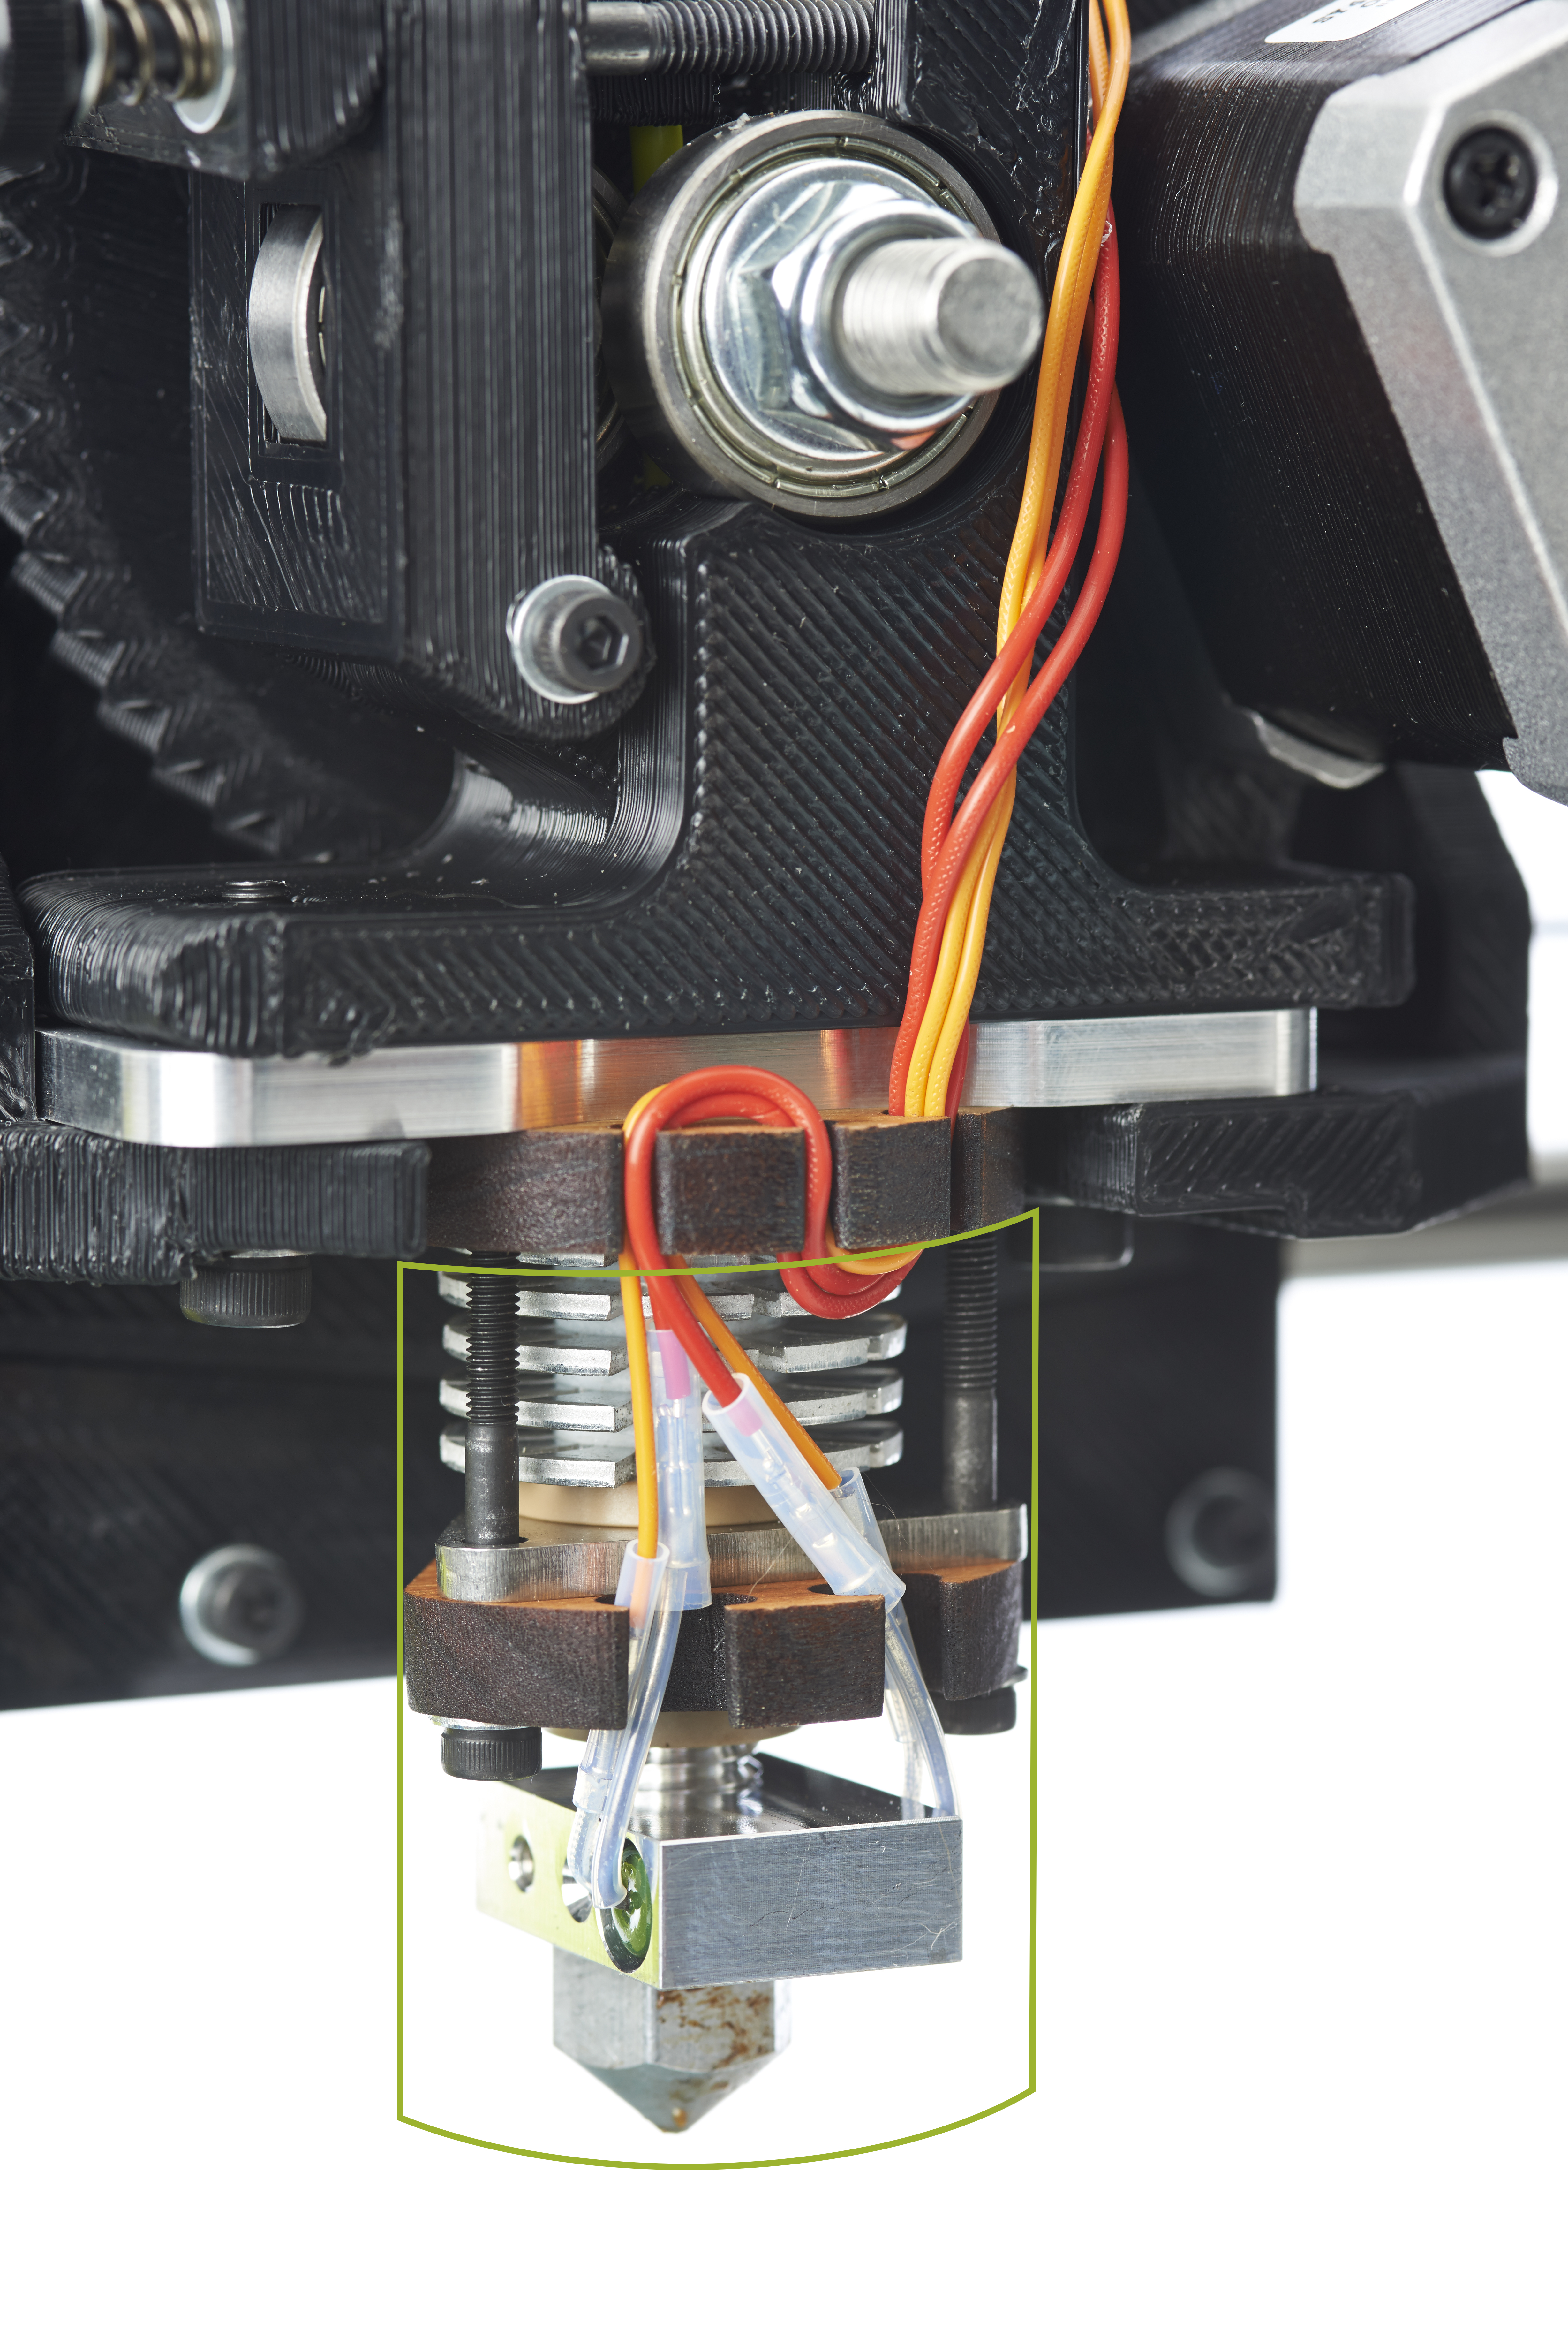
\includegraphics[width=0.5\textwidth]{simple_mode/extruder_clearance.JPG}
\caption{A diagram depicting the clearance around an extruder.}
\label{fig:a_diagram_depicting_extruder_clearance}
\end{figure}
% paragraph sequential_printing (end)


\subsubsection{Filament Settings}

The \texttt{Filament Settings} will normally be used infrequently, for example on receipt of a new roll of filament.

\begin{figure}[H]
\centering
\includegraphics[width=\textwidth]{simple_mode/simple_mode_filament_settings.png}
\caption{Simple Mode: Filament Settings.}
\label{fig:simple_mode_filament_settings}
\end{figure}

\paragraph{Filament.} % (fold)
\label{par:filament}
The \texttt{Diameter} setting will already have been filled from the value given during the wizard (see p.\pageref{sub:4_filament_diameter}), but can be updated here.

The \texttt{Extrusion multiplier} setting allows the fine tuning of the extrusion rate.  Whilst the value should ideally be set in the firmware it can be useful to test slight changes to the rate by altering this value.
% paragraph filament (end)

\paragraph{Temperature.} % (fold)
\label{par:temperature}
These values are also filled from the wizard, but here the opportunity exists to set the temperature for the first layer (see p.\pageref{sec:the_important_first_layer}).
% paragraph temperature (end)


\subsubsection{Printer Settings}

The \texttt{Printer Settings} will be updated the least, unless Slic3r is going to be used for many printers, for example, in a 3D printer farm.

\begin{figure}[H]
\centering
\includegraphics[width=\textwidth]{simple_mode/simple_mode_printer_settings.png}
\caption{Simple Mode: Printer Settings.}
\label{fig:simple_mode_printer_settings}
\end{figure}

\paragraph{Size and coordinates.} % (fold)
\label{par:size_and_coordinates}
The \texttt{Bed size} setting is taken from the wizard (see p.\pageref{sub:2_bed_size}), and the \texttt{Print center} is simply the mid-point of these values.  \texttt{Z offset} can be used to compensate for an incorrectly calibrated Z end-stop.  If the nozzle stops slightly too far from the bed, then adding a negative value will offset all layers by that amount.  The real solution however is to fix the end-stop itself.
% paragraph size_and_coordinates (end)

\paragraph{Firmware.} % (fold)
\label{par:firmware}
As selected in the wizard (see p.\pageref{sub:1_firmware_type}), \texttt{G-code flavour} defines the dialect of G-code generated.
% paragraph firmware (end)


\paragraph{Extruder.} % (fold)
\label{par:extruder}
\texttt{Nozzle diameter} was defined in the wizard (see p.\pageref{sub:3_nozzle_diameter}).
% paragraph extruder (end)

\paragraph{Retraction.} % (fold)
\label{par:retraction}
Unless the material being extruded has a very high viscosity it will ooze between extrusions due to gravity.  This can be remedied against by reducing the time between extrusions, and by actively retracting the filament between extrusions.  Setting the \texttt{Length} parameter to a positive value will cause the filament to be reversed by that many millimeters during travel.

Setting the \texttt{Lift Z} parameter to a positive value will raise the entire extruder on the Z axis by that many millimeters during each travel.  This can be useful to ensure the nozzle will not catch on any already laid filament.
% paragraph retraction (end)

\paragraph{Start G-code.} % (fold)
\label{par:start_g_code}
Custom gcode commands that run before the print run starts.  Some common gcodes to use are:
\begin{itemize}
	\item \textbf{G28}  - Homes all the axes.
\end{itemize}
The RepRap wiki is a good resource to learn about the variety of gcodes available: \texttt{http://reprap.org/wiki/G-code}.  

Note: Be sure to check that a given gcode is valid for your firmware.
% paragraph start_g_code (end)

\paragraph{End G-code.} % (fold)
\label{par:end_g_code}
Custom gcode commands that run after the print run ends.  Some common gcodes to use are:
\begin{itemize}
	\item \textbf{M104 S0}  - Sets the extruder temperature to zero.
	\item \textbf{M140 S60}  - Sets the heat bed temperature to sixty.
	\item \textbf{G28 X0} - Home the X axis.
	\item \textbf{M84}  - Disables the motors.
\end{itemize}
% paragraph end_g_code (end)


\input{slic3r/WorkingWithModels}

%!TEX root = Slic3r-Manual.tex

\input{slic3r/Calibration}

\newpage

\input{slic3r/ConfigurationWizard}

\newpage

\input{slic3r/FirstLayer}

\newpage

\input{slic3r/WorkingWithModels}

\newpage

\input{slic3r/Printing}



\section{Configuration Tuning}
%!TEX root = Slic3r-Manual.tex

%!TEX root = Slic3r-Manual.tex

\subsection{Infill Choices} % (fold)
\label{sec:infill_choices}
\index{infill}

There are several considerations when choosing an infill pattern: object strength, time, material, and personal preference.  It can be inferred that a more complex pattern will require more moves, and hence take more time and material.  

Slic3r offers several infill patterns, four regular, and three more exotic flavours.  The numbers given in brackets below each figure are a rough estimate of material used and time taken for a simple 20mm cube model\footnote{Taken from http://gcode.ws}.  Note that this is only indicative, as model complexity and other factors will affect time and material.

\begin{figure}[H]
\centering
\includegraphics[keepaspectratio=true,width=0.2\textwidth]{tuning/infill_line.png}
\caption{Infill pattern: Line (344.51mm / 5m:20s)}
\label{fig:infill_line}
\end{figure}

\begin{figure}[H]
\centering
\includegraphics[keepaspectratio=true,width=0.2\textwidth]{tuning/infill_rectilinear.png}
\caption{Infill pattern: Rectilinear (350.57mm / 5m:23s)}
\label{fig:infill_rectilinear}
\end{figure}

\begin{figure}[H]
\centering
\includegraphics[keepaspectratio=true,width=0.2\textwidth]{tuning/infill_concentric.png}
\caption{Infill pattern: Concentric (351.80mm / 5m:30s)}
\label{fig:infill_concentric}
\end{figure}

\begin{figure}[H]
\centering
\includegraphics[keepaspectratio=true,width=0.2\textwidth]{tuning/infill_honeycomb.png}
\caption{Infill pattern: Honeycomb (362.73mm / 5m:39s)}
\label{fig:infill_honeycomb}
\end{figure}

\begin{figure}[H]
\centering
\includegraphics[keepaspectratio=true,width=0.2\textwidth]{tuning/infill_hilbertcurve.png}
\caption{Infill pattern: Hilbert Curve (332.82mm / 5m:28s)}
\label{fig:infill_hilbertcurve}
\end{figure}

\begin{figure}[H]
\centering
\includegraphics[keepaspectratio=true,width=0.2\textwidth]{tuning/infill_archimedeanchords.png}
\caption{Infill pattern: Archimedean Chords (333.66mm / 5m:27s)}
\label{fig:infill_archimedeanchords}
\end{figure}

\begin{figure}[H]
\centering
\includegraphics[keepaspectratio=true,width=0.2\textwidth]{tuning/infill_octagramspiral.png}
\caption{Infill pattern: Octagram Spiral (318.63mm / 5m:15s)}
\label{fig:infill_octagramspiral}
\end{figure}


Certain model types are more suited for a particular pattern, for example organic versus mechanical types.  Figure \ref{fig:complex_object_infill_comparison} shows how a honeycomb fill may suit this mechanical part better because each hexagon bonds with the same underlying pattern each layer, forming a strong vertical structure.

\begin{figure}[H]
\centering
\includegraphics[keepaspectratio=true,width=0.75\textwidth]{tuning/complex_object_infill_comparison.png}
\caption{Infill pattern comparison in a complex object. Left to Right: honeycomb, line}
\label{fig:complex_object_infill_comparison}
\end{figure}

Most models require only a low density infill, as providing more than, say, 50\% will produce a very tightly packed model which uses more material than required.  For this reason a common range of patterns is between 10\% and 30\%, however the requirements of the model will determine which density is best.  Figure \ref{fig:infill_pattern_densities} shows how the patterns change as the density increases.
\begin{figure}[H]
\centering
\includegraphics[keepaspectratio=true,width=0.7\textwidth]{tuning/infills.png}
\caption{Infill patterns at varying densities. Left to Right: 20\%,40\%,60\%,80\%. Top to Bottom: Honeycomb, Concentric, Line, Rectilinear, Hilbert Curve, Archimedean Chords, Octagram Spiral}
\label{fig:infill_pattern_densities}
\end{figure}

One aspect to consider is how well the material which makes up the top layer bridges the infill pattern.  Should the pattern have wide gaps then the material may sag and break in between, causing unfinished top surfaces.

\begin{figure}[H]
\centering
\includegraphics[keepaspectratio=true,width=0.75\textwidth]{tuning/bad_top_infill.JPG}
\caption{Image of a poorly top-filled print.}
\label{fig:poor_top_fill}
\end{figure}

This problem can be mitigated by calibrating optimal bridging and/or by increasing the number of solid top layers (see p.\pageref{par:simple_general}).

% section infill_choices (end)


%!TEX root = Slic3r-Manual.tex

\subsection{Speeding Things Up} % (fold)
\label{sec:speeding_things_up}
\index{speed}

Once the printer is reliably producing good quality prints it may be desirable to increase the speed.  Doing this provides several benefits, the most obvious of which is that the results are produced quicker, but also faster print times can be utilised in producing more layers, i.e. lower layer height, thus improving perceived print quality.  An additional benefit is that a faster travel movement, between extrusions, can reduce the effects of oozing.

The best approach is to increment the various speed parameters in small steps and observe the effect each change has on print quality.  Travel speed is a safe starting point, and it is not unrealistic to attain speeds of up to 250mm/s (if your printer can handle it).  Adjusting the speed of perimeters, infill is available in simple mode, and the general rule is to have the perimeter go a little slower than the infill in order to reduce possible blemishes on the surface (infill can be faster because slight gaps will not matter as much).

Expert mode offers more parameters to fine tune printer speeds.  Differentiation between external, small and other perimeters, infill locations, and bridges and gaps are available, as well as the ability to slow down for the first layer.

\begin{figure}[H]
\centering
\includegraphics[keepaspectratio=true,width=0.75\textwidth]{tuning/speed_advanced_settings.png}
\caption{Expert mode speed options.}
\label{fig:speed_advanced_settings}
\end{figure}

Where indicated a value can be given in percentage.  This is in relation to the preceding value, e.g. 50\% solid infill would be half of the value defined for infill.

A few general guidelines for each option:
\begin{itemize}
	\item \texttt{Perimeters}  - In expert mode this parameter can be increased slightly as the \texttt{External perimeters} option can be used to ensure blemish free external faces.
	\item \texttt{Small perimeters}  - Meant for holes, islands and fine details, a slower speed here is recommended.
	\item \texttt{External perimeters}  - A slightly slower value may ensure cleaner surfaces.
	\item \texttt{Infill}  - As fast as you can without compromising the integrity of the fill structure.  Faster extrusions can break and result in weak spots.
	\item \texttt{Solid infill}  - The bottom of the model, and any additional solid layers is usually slightly slower than infill but faster than perimeters.
	\item \texttt{Top solid infill}  - Allow time for the extrusion to cleanly cover the previous top layers and result in a tidy top surface.  the last few layers should have bridged the infill structure nicely, preparing the way for a neat finish. 
	\item \texttt{Support material}  - Generally support structures are quick and dirty, and so long as the base is adequately supported they can be built as quickly as they can.
	\item \texttt{Bridges}  - Having the extrusion span distances depends on the material and cooling.  Going too slow will result in sagging, too fast will result in broken strands.  Experimentation is the key here, but generally bridging runs slower than perimeters.
	\item \texttt{Gap fill}  - Filling in small gaps results in the extruder quickly oscillating and the resulting shaking and resonance could have a detrimental affect on the printer.  A smaller value here can guard against this. 
	\item \texttt{Travel}  - As fast as your printer will allow in order to minimise ooze.
	\item \texttt{First layer speed}  - As mentioned in section \ref{sec:the_important_first_layer}, the first layer is important to lay down correctly, and a slower pace helps enormously.  Setting a value of 50\%, or even less, can really help.
\end{itemize}

\texttt{Acceleration control} is an advanced setting allowing acceleration settings for perimeters, infill, bridge, as well as a default setting, to be made.  Deciding which values to set depends on the capabilities of the machine.  Any settings within the firmware may be a good starting point.

Take into account any restrictions enforced by the firmware as many have settings for the maximum safe speed of each axis.

Care must be taken when increasing the speed with regard to the printing of small models, as the speed of the extruder nozzle relates to how the material cools, and the smaller the model the closer the hot-end stays to the freshly extruded plastic.  Generally smaller models, or those with fine details, benefit from slower extrusion speeds.  Patience is, as they say, a virtue!

A further consideration is how fast can the material be pushed through the extruder.  The power of the hot-end and the length of the hot zone will determine whether it can melt the material sufficiently at high extrusion speeds.  Each hot-end will have it's upper limit which can be found through trial and error or by asking the supplier or community.  For those making their own hot-ends it is worth looking at RichRap's work with high-speed extrusion\footnote{http://richrap.blogspot.de/2011/08/high-power-hot-end-for-fast-printing.html}.

% section speeding_things_up (end)


%%!TEX root = Slic3r-Manual.tex

\subsection{Cooling Things Down} % (fold)
\label{sec:cooling_things_down}
\index {cooling}

Temperature plays a key part in determining print quality.  Too hot and the material deforms, too cool and layer adhesion may be problematic.  Applying a cooling technique will allow the freshly deposited material to solidify enough to provide a good base for the next layer, helping with overhangs, small details and bridges.

There are two main techniques for cooling: adding a fan, or slowing down the print speed.  

\subsubsection{Fans} % (fold)
\label{sub:fans}
Most electronics and firmware allow the addition of a fan via a spare connector.  These can then be instructed with G-code, from Slic3r, to turn on or off as the model requires, and to rotate at different speeds.

Care should be taken with the positioning of the fan so that it does not cool any heated bed more than necessary.  It should also not cool the heater block of the hot-end so as not to force it to do more work and waste energy.  The air movement should aim for the nozzle tip, flowing over the freshly extruded material. 

\begin{figure}[H]
\centering
\includegraphics[keepaspectratio=true,width=0.75\textwidth]{placeholder.jpg}
\caption{Ideal fan placement.}
\label{fig:ideal_fan_placement}
\end{figure}

A duct may help in guiding the flow correctly, and there are several designs available online, for a wide variety of printers.

% subsection fans (end)

\subsubsection{Slowing Down} % (fold)
\label{sub:slowing_down}
Slic3r can tell the printer to slow down if the estimated layer time is above a certain threshold.

Care must be taken as the intended effect could be mitigated by the nozzle not moving far enough away from the fresh extrusion, a problem with small, detailed layers.  For this reason it is usually recommended to use a fan where possible.
% subsection slowing_down (end)


\subsubsection{Configuring} % (fold)
\label{sub:configuring_cooling}

In simple mode Slic3r will attempt to choose the optimal settings for both fans and speed.  Expert mode gives more granular options.  

\begin{figure}[H]
\centering
\includegraphics[keepaspectratio=true,width=0.75\textwidth]{tuning/cooling_advanced_settings.png}
\caption{Cooling advanced settings.}
\label{fig:cooling_advanced_settings}
\end{figure}

\begin{itemize}
	\item \textbf{Fan speed}  - Determines the minimum and maximum speeds - useful for fans that run too fast by default.
	\item \textbf{Bridges fan speed}  - As the material stretches over wide gaps, it makes sense to try and cool it as much as possible, therefore a full fan speed is recommended.
	\item \textbf{Disable fan for first \textit{x} layers}  - Section \ref{sec:the_important_first_layer} detailed how important the first layer is, and so it makes sense not to apply the fan until sure the print is securely attached to the bed.  Keeping the fan turned off for the first two or three layers is a good idea.
	\item \textbf{Keep fan always on}  - Overrides any other choices and has the fan run continuously, at least at the minimum speed setting.  This can be useful when printing with PLA, but is not recommended for ABS.	
\end{itemize}

\begin{itemize}
	\item \textbf{Enable fan if print time is below \textit{t} seconds}  - Triggers the fan if the layer will be completed within the given number of seconds.
	\item \textbf{Slow down if layer print time is below \textit{t} seconds}  - Slows down the print if the layer will be completed within the given number of seconds.
	\item \textbf{Min print speed}  - A lower limit on how slowly a layer can be printed. 
\end{itemize}


% subsection configuring_cooling (end)

% section cooling_things_down (end)


%!TEX root = Slic3r-Manual.tex

\subsection{Brim and Raft} % (fold)
\label{sec:brim_and_raft}

\subsubsection{Brim} % (fold)
\label{sub:brim}
\index{brim}

Both simple and expert mode gives the option to add a brim to the first layer of the print.  This is simply additional perimeters around the outside of the model which increases the amount of material holding onto the bed in an effort to reduce warping.  It is also useful for increasing the surface area of small yet tall prints which may otherwise be knocked off the bed mid-print.

Once completed the brim is removed from the print using a sharp utility knife or scalpel.

\begin{figure}[H]
\centering
\includegraphics[keepaspectratio=true,width=0.75\textwidth]{tuning/brim.JPG}
\caption{Print with brim.}
\label{fig:print_with_brim}
\end{figure}

% subsection brim (end)

\begin{comment}

\subsubsection{Raft} % (fold)
\label{sub:raft}
\index{raft}

A technique dating back to the early days of 3D printing, a raft is a support structure printed underneath the model.  Because the raft extrusion is usually quite wide it adds more surface area for the print, and additionally covers any surface irregularities in the bed material, should they exist.  The raft technique is particularly popular when printing with ABS as it tends to warp more than PLA.

Again, the raft is expected to be removed manually after the print is completed.

A raft is added by turning on the support option and configuring how many layers should be printed to make up the raft.  As with support structures, the raft is printed rather loosely and the model is not pressed into it too much, in order that it may be easily removed afterwards.

\begin{figure}[H]
\centering
\includegraphics[keepaspectratio=true,width=0.75\textwidth]{placeholder.jpg}
\caption{Print with raft.}
\label{fig:print_with_raft}
\end{figure}

\end{comment}

% subsection raft (end)

% section brim_and_raft (end)



\section{Configuration Organization}
\input{slic3r/Organize}

\section{Advance Slicing}
%!TEX root = Slic3r-Manual.tex

\input{SVGOutput}

\input{CommandLineUsage}

\input{PostProcessingScripts}


%\section{Troubleshooting}
%Troubleshooting

\subsection{Common Issues}

Z wobble

Z wobble due to motor steps not matching Z rods thread pitch, see \texttt{http://evernote.com/shard/s211/sh/701c36c4-ddd5-4669-a482-953d8924c71d/1ef992988295487c98c268dcdd2d687e}

Overhangs and the top layers.

First Layer Sticking

Blobbing

Poor layer adhesion



\section{The Cutting Edge of Slicer}
\input{slic3r/Edge}
}
\fi
%%% END SLIC3R %%%
\end{comment}


%%% FIRSTPRINT %%%
\iffirstprint
\chapter{\emph{Your First 3D Print}}
\label{firstprint}
\thispagestyle{empty}
\markboth{Your First 3D Print}{LulzBot\textsuperscript{\miniscule{\texttrademark}} TAZ User Manual}
{\index{bed leveling}
\section{Bed Leveling}
Make sure you take the time to go through the following procedure to help ensure that your prints are consistent and trouble free. Make sure to first read the instructions for using the Printrun software. Connect to the printer as described in the Printrun software section. Once \texttt{Pronterface} is connected to the printer use the homing buttons to home the X and Y axis. \color{red}{Do not use the \texttt{HomeZ button}until after the \texttt{Z axis End stop} has been adjusted. Make sure that the red shipping clamps on the Z axis smooth rods have been removed before continuing.}

\index{z axis}
\subsection{Lowering the Z Axis}
Once connected to the TAZ 3D printer in Pronterface, Use the \texttt{-Z 1 button} to move the Z axis down in \texttt{1mm} increments. Move the Z axis down towards the bed by 5mm at first. While the Z axis is moving down pay attention to the Z axis movement and sound. The Z axis stepper motors should be moving in unison. If you notice a grinding sound stop and, before proceeding, make sure that the Z axis looks level in relation to the body of the TAZ 3D printer. Once you have confirmed smooth movement of the Z axis, use the \texttt{-Z 10 button} to move the Z axis down in 10mm increments. \textcolor{red}{Commands sent in Pronterface will stack, so multiple movement button presses can potentially be harmful and cannot be stopped without powering down the 3D printer.} Keep an eye on the nozzle for the hot end. As it approaches the surface of the bed use the \texttt{-Z 1 button} to continue lowering the Z axis into position. Stop lowering the Z axis once the Z axis has been lowered to within 4 inches(100mm) of the bed.

\subsection{Verify Z Axis Leveling}
With the Z axis lowered near the bed, use the included \texttt{150mm ruler} to measure the distance from the bottom of the \texttt{X axis} smooth rod and the top surface of the \texttt{Y axis} aluminum bed plate on the left side.
\begin{figure}[H]
\centering
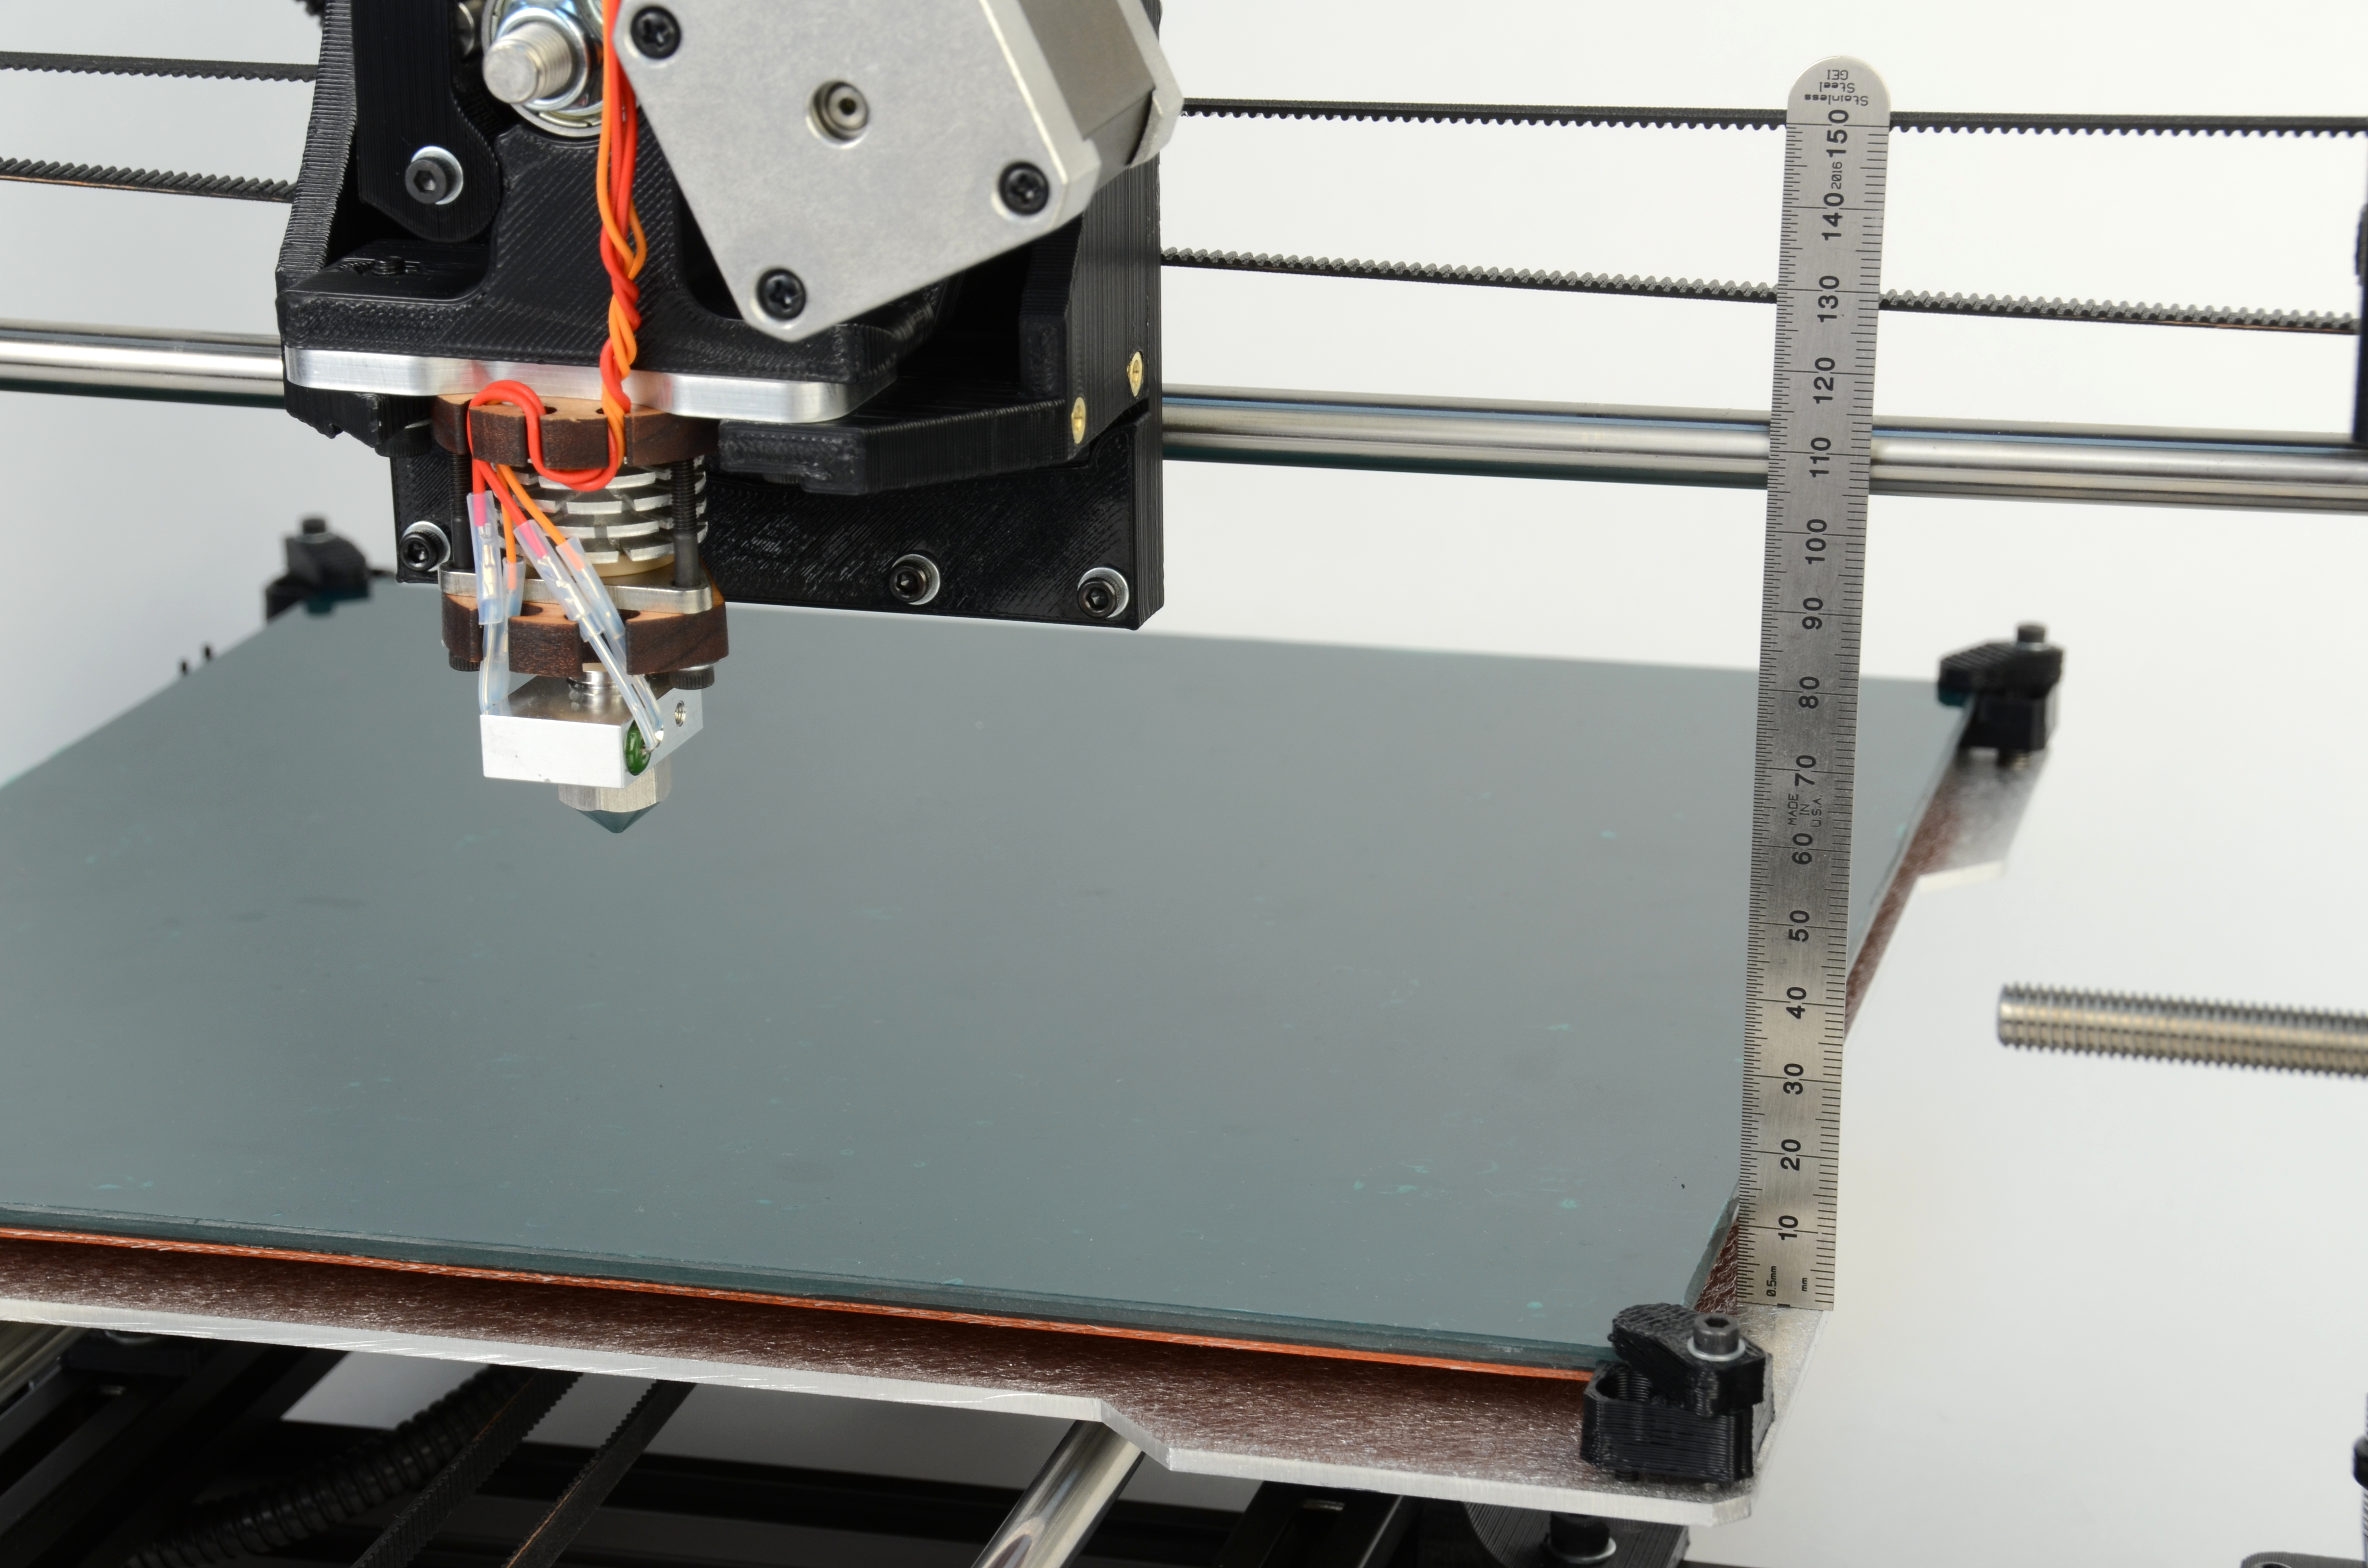
\includegraphics[keepaspectratio=true,angle=0,height=0.4\textheight,width=1.0\textwidth]{X-Y_axes_leveling_check.JPG}
\caption{Verifying the X and Y axis are square}
\label{fig:X-Y_axes_leveling_check}
\end{figure} 
Compare the distance measurement from the left side to the measurement on the right side. The distance measurement should be the same. If not, in Pronterface use the \texttt{Motors off} button to turn off the stepper motors on the TAZ 3D printer. Manually, by hand, turn the threaded rod on one side of the printer to raise or lower that side to match the measurement on the other side. If the Z axis has been adjusted measure again to confirm that the left and right side of the Z axis are level in relation to the Y axis aluminum plate.

\subsection{Rough Adjustment of the Z Axis End Stop}
\index{end stop}
Before using the \texttt{home Z} button or the \texttt{home all} button you will need to adjust the \texttt{Z axis endstop}.
\begin{figure}[p]
\centering
\includegraphics[keepaspectratio=true,angle=0,height=0.4\textheight,width=1.0\textwidth]{Z_end_stop_trigger.JPG}
\caption{Z end stop trigger}
\label{fig:Z_end_stop_trigger}
\end{figure}
Rotate the \texttt{Z axis end stop trigger} clockwise to lower the bottom of the screw closer to the Z axis end stop. Once lowered by approximately 1cm, press the \texttt{HomeZ button} to home the Z axis. The hot end will approach the heated bed and will likely stop around a centimeter above the surface of the heated bed.

\subsection{Fine Adjustment of the Z Axis End Stop}
Adjust the \texttt{Z axis end stop trigger} by rotating the screw counter-clockwise to raise the tip of the screw. Raise the screw by roughly the same amount of the distance between the nozzle tip and the print surface. Press the \texttt{Home Z}button to home the Z axis. The tip of the nozzle should now be very close to the surface of the bed.

\subsection{Leveling the Print Bed}
Slide a thin piece of paper underneath the nozzle in the front left corner of the bed. Adjust the z axis end stop and home the Z axis until the tip of the nozzle applies a firm pressure on the paper. Try to slide the paper from underneath the the tip of the nozzle. It should not tear, but some resistance should be felt. Move the hot end nozzle tip over to the far side of the X axis by using the \texttt{+X 100 button}. As the X axis carriage approaches the end of the X axis use the \texttt{+X 10 button} and finally the \texttt{+X 1 button}. Once the tip of the nozzle is near the front right corner of the bed slide the same piece of paper under the nozzle and home the Z axis. To raise or lower the front right corner of the bed adjust the third screw from the left. Do not adjust the middle screw. Adjust the front right corner of the bed until the amount of tension felt when moving the piece of paper under the nozzle feels the same as the tension felt when doing the same thing on the front left corner. Repeat the same process using the \texttt{+Y button} to move the heated bed to place the nozzle on the rear right corner of the bed. Adjust the height of the bed using the same procedure as outlined above. Finally, move the X axis carriage over to the rear left corner of the bed and perform the same leveling procedure to adjust the last corner. The bed should now be almost perfectly level. We will check this in a later section. Use the controls in Printrun to raise the Z axis up 20mm, and move the X axis carriage over to the center of the X axis.

\section{Set Temperature}
\index{temperature}
%Make sure to first read the instructions for using the Printrun software. Connect to the printer as described in the Printrun software section
%%% XXX pageref going to \label not \section (page \pageref{Installing Printrun}).
Set the hot end and print surface for ABS or PLA plastic and turn both on. The temperature settings for ABS should be set at \texttt{230°C} for the hot end and \texttt{85°C} for print surface; for PLA they should be set at \texttt{185°C} for the hot end and \texttt{55°C} for print surface. Click the \texttt{Motors Off} button.
\glossary{Idler}{Refers to parts using a bearing (usually a 608ZZ) to add tension in belts or to add pressure against a rolling surface.}
\section{Load Filament}
\index{filament}
\index{hot end}

Once the hot end is heated to the correct temperature you will now need to load the plastic filament into the extruder. Raise both the idler clip and the 2 screws adding tension to release the hinged idler. It can be loosened if necessary. If the extruder has a small section of filament already loaded, you will need to remove the filament once the extruder idler has been opened by gently pulling out the filament by hand once the hot end has reached the extrusion temperature of \texttt{230C}
(Fig. \ref{fig:extruder_idler_release}).
\begin{figure}[hbt]
\centering
\includegraphics[keepaspectratio=true,angle=0,height=0.4\textheight,width=1.0\textwidth]{extruder_idler_release.JPG}
\caption{Extruder idler release}
\label{fig:extruder_idler_release}
\end{figure}
% update feed hole picture.
Gently squeeze both the idler screws and the plastic clip together and pull upwards to release the idler. The idler can be rotated downwards allowing access to the hobbed bolt and filament feed hole(Fig. \ref{fig:extruder_filament_slot}, page \pageref{fig:extruder_filament_slot}). Feed the end of the plastic filament into the filament feed hole
(Fig. \ref{fig:extruder_filament_slot}).
\begin{figure}[hbt]
\centering
\includegraphics[keepaspectratio=true,angle=0,height=0.4\textheight,width=1.0\textwidth]{extruder_filament_slot.JPG}
\caption{Extruder filament slot}
\label{fig:extruder_filament_slot}
\end{figure}
Now you can push the filament through the extruder by slowly pushing the filament down into the hot end.

Once the filament extrudes a small amount out of the nozzle raise the idler and slide the two idler bolts and plate back into place. Tighten the two idler bolts if you previously loosened them. Tighten the two screws until they are finger tight, then tighten them slightly more. Now use the \texttt{Extrude} button in Printrun to test that the extruder is working properly. You may need to extrude 40-60mm of filament to fully prime the hot end. Adjust the tension on the two screws until you can reliable and repeatedly extrude roughly 40mm of filament.

\section{Home Printer}
Use the home buttons to home the X axis and then the Y axis. Next home the Z axis. When the Z axis is at home the nozzle tip should be sitting right against the glass
(Fig. \ref{fig:nozzle_height}, page \pageref{fig:nozzle_height}). The image to the right, in figure \ref{fig:nozzle_height}, is the correct nozzle height.
\begin{figure}[p]
\centering
\includegraphics[keepaspectratio=true,angle=0,height=0.4\textheight,width=1.0\textwidth]{nozzle_height.jpg}
\caption{Nozzle height}
\label{fig:nozzle_height}
\end{figure}
\begin{figure}[p]
\centering
\includegraphics[keepaspectratio=true,angle=0,height=0.4\textheight,width=1.0\textwidth]{Z_end_stop_trigger.JPG}
\caption{Z end stop trigger}
\label{fig:Z_end_stop_trigger}
\end{figure}
The nozzle should not be pushing down on the print surface. To lower or raise the Z home height adjust the Z end stop trigger. The red end stop trigger is on the far left of the printer mounted on the X-axis motor mount.
(Fig. \ref{fig:Z_end_stop_trigger}, page \pageref{fig:Z_end_stop_trigger}).
The red end stop trigger can be lowered by turning clockwise and raised by turning counter-clockwise. Once you have homed the axes and the hot end and bed have reached the correct temperature it is time to print!

%fix image positioning, images for 5.3 get shoved underneath 5.4
\section{Z Print Height}
Load the \texttt{bedcalib.gco} file.
This file can be found at:
\texttt{http://download.lulzbot.com/TAZ/calibration/bed_level.gcode} once downloaded you your computer press the \texttt{Load file button}. Navigate through the file browser to the downloaded \texttt{bed_level.gcode} file.

The .gcode file should appear in the Printrun G-Code viewer. Press the \texttt{Print} button to begin the print. When the print starts make sure the first layer is not printing too close or too far from the print bed. Note 
Figure \ref{fig:1st_layer_adhesion}, page \pageref{fig:1st_layer_adhesion},
\begin{figure}[hbt]
\centering
\includegraphics[keepaspectratio=true,angle=0,height=0.4\textheight,width=1.0\textwidth]{1st_layer_adhesion.jpg}
\caption{First layer adhesion}
\label{fig:1st_layer_adhesion}
\end{figure}
as an example of a good first layer adhesion. From left to right: very low, low, \emph{perfect,} high, very high. If the first layer is too high or low you can pause the print by pressing the \texttt{Pause} button. Adjust the Z end stop trigger. After making adjustments remove any printed material off the bed and home the axes and press \texttt{Restart} to restart the print. Measure the extrusion width, ideally the width would be the same in all areas of the bed. You would raise/lower a corner to minimize/increase the extrusion width to match the others. Once they are all consistent, the bed is level.

\section{Your First Print!}
Load the \texttt{octopus.gcode} file.
This file can be found at:
\texttt{http://download.lulzbot.com/TAZ/novelties/octopus.gcode}. Load the file in Pronterface, bring the hot end \texttt{(230C ABS/185C PLA))} and the heated bed \texttt{(85C ABS/60C PLA)} up to printing temperature. Once the printer is at the appropriate temperature, press the \texttt{Print} button to begin the print.

\section{Remove Part}
After the part is finished printing, the heated bed will automatically cool down to \texttt{60°C}. If you are printing PLA you will need to turn the heated bed off. Once the bed cools you can you pop the finished part off of the printed surface. To remove the printed part, use the clam knife included in your printer kit. Leather gloves are suggested to protect your hands from the clam knife blade. It is also safe practice to not place your hand behind the direction you are pushing the clam knife. Using the side of the clam knife blade pry up one side of the printed part. If your part is large you may need to pry at multiple points to pop the part off of the print surface. When removing parts take caution to not damage the PET film. If the film is cut or ripped it will peel from the glass and need to be replaced. Make sure to reset the heated bed to the correct temperature and allow it to heat up to the needed temperature before starting the next print.


\fi
%%% END FIRSTPRINT %%%

%%% SLIC3R %%%
\ifsoftware
\chapter{\emph{Slic3r}}
\thispagestyle{empty}
\markboth{Slic3r}{LulzBot\textsuperscript{\miniscule{\texttrademark}} TAZ User Manual}
{\section{Intro}
\input{slic3r/Intro}

\section{Getting Slic3r}
\input{slic3r/Getting}

\section{First Slice}
%!TEX root = Slic3r-Manual.tex

LulzBot provides ready-made Slic3r profiles for immediate use to get printing quickly. You can find the TAZ Slic3r profiles at \texttt{http://download.lulzbot.com/TAZ/software/current/slic3r/config/}. Once you have become familiar with your TAZ printer and the software you may want to make your own profiles with slight adjustments for particular designs.

%%!TEX root = Slic3r-Manual.tex

\subsection{\texttt{Calibration}}
\label{calibration}
\index{calibration}

Your LulzBot\textsuperscript{\miniscule{\texttrademark}} TAZ 3D printer was calibrated at the factory prior to packing. TAZ users do not need to calibrate their printers. 

% Uncomment section below for standalone Slic3r manual. Should never be needed for LulzBot assembled products.
%Before even attempting the first print it is vital that the printer is correctly calibrated. Skipping or rushing this step will result in frustration and failed prints later, so it is important to take the time to make sure the machine is correctly set up. Be sure to complete the Setup and First Print section of this manual before moving forward with Slic3r.

If you are just beginning with 3D printing or Slic3r, LulzBot\textsuperscript{\miniscule{\texttrademark}} recommends starting with our pre-set Slic3r profiles. You can find the TAZ Slic3r profiles at \texttt{https://www.lulzbot.com/Slic3r}. For information on loading and export Slic3r profiles please see page \pageref{sub:exporting_and_importing_configuration}. Note that the pre-set profiles will only work correctly when Slic3r is in Expert mode.

The pre-set profiles will give you Slic3r settings that will work great on most designs. The Slic3r manual can be used as a reference in building knowledge of Slic3r settings while using the pre-set profiles. Once you have a number of prints completed you can use the Slic3r manual as a reference to make small adjustments to the pre-set profiles or begin creating your own profiles.


%!TEX root = Slic3r-Manual.tex

\subsection{\texttt{Configuration Wizard}}
\label{sec:configuration_wizard}
\index{Configuration Wizard}

Slic3r has two features to aid newcomers: the configuration wizard, and simple mode.

Sometimes it is nice to have a helping hand when starting out with new software.  The configuration wizard asks a series of questions and creates a new configuration for Slic3r.

\textbf{When using the pre-set TAZ Slic3r profiles you do not need to complete the Configuration Wizard.} The Configuration Wizard can be later accessed from the top menu once you are ready to start creating your own Slic3r profiles.

\begin{figure}[H]
\centering
\includegraphics[keepaspectratio=true,width=\textwidth]{configuration_wizard/configuration_wizard_welcome.png}
\caption{Configuration Wizard: Welcome Screen}
\label{fig:configuration_wizard_welcome_screen}
\end{figure}

\newpage
\subsubsection{\texttt{1. Firmware Type}}
\label{sub:1_firmware_type}
\index{Printer Settings!Firmware!G-code flavour}
The gcode produced by Slic3r is tailored to particular types of firmware.  The first step prompts for the firmware that the printer uses.  For the TAZ printer select \texttt{RepRap (Marlin/Sprinter)}
\begin{figure}[H]
\centering
\includegraphics[keepaspectratio=true,width=\textwidth]{configuration_wizard/configuration_wizard_firmware_type.png}
\caption{Configuration Wizard: Firmware Type}
\label{fig:configuration_wizard_firmware_type}
\end{figure}

\newpage
\subsubsection{\texttt{2. Bed Size}}
\label{sub:2_bed_size}
\index{Printer Settings!Size and coordinates!Bed size}
This setting defines the maximum distance the extruder may travel along the X and Y axis.  The dimensions for the TAZ print surface are X: 298 and Y: 275.

Be sure to measure from the lower left corner where the extruder nozzle rests when are the home position to the maximum distance the nozzle can travel in each direction.  Take into account that the X carriage may touch the frame before the nozzle reaches it's full distance, this will depend on the printer make and model.

\begin{figure}[H]
\centering
\includegraphics[keepaspectratio=true,width=\textwidth]{configuration_wizard/configuration_wizard_bed_size.png}
\caption{Configuration Wizard: Bed Size}
\label{fig:configuration_wizard_bed_size}
\end{figure}

\newpage
\subsubsection{\texttt{3. Nozzle Diameter}}
\label{sub:3_nozzle_diameter}
\index{Printer Settings!Extruder!Nozzle diameter}
The diameter of the hot-end nozzle is usually clearly displayed either in the description of the hot-end, or in the associated documentation, when the hot-end is purchased.  The nozzle sizes available for the TAZ hot end are 0.35mm and 0.50mm.

If the nozzle was home-made, or came from a source without a diameter given, then carefully measure the aperture as accurately as possible.  One way of determining nozzle size is to very slowly (1mm/s) extrude some filament into free air and measure the thickness of the resulting extrusion\footnote{\	http://forums.reprap.org/read.php?1,113374,113953}.  This has the benefit of taking die swell into account, and consequently may be a useful thing to do even if the diameter is known.

\begin{figure}[H]
\centering
\includegraphics[keepaspectratio=true,width=\textwidth]{configuration_wizard/configuration_wizard_nozzle_diameter.png}
\caption{Configuration Wizard: Nozzle Diameter}
\label{fig:configuration_wizard_nozzle_diameter}
\end{figure}

\newpage
\subsubsection{\texttt{4. Filament Diameter}}
\label{sub:4_filament_diameter}
\index{Filament Settings!Filament!Diameter}
For Slic3r to produce accurate results it must know as accurately as possible how much material is pushed through the extruder.  Therefore it is vital to give it as precise a value as possible for the filament diameter.

Although the filament used in FDM printers is sold as being either 3mm or 1.75mm this is only a general guide.  The diameter can vary between manufacturers and even between batches.  Therefore it is highly recommended to take multiple measurements from along a length of the filament and use the average.  For example, measurements of 2.89, 2.88, 2.90 and 2.91 would yield an average of 2.895, and so this would be used.

\begin{figure}[H]
\centering
\includegraphics[keepaspectratio=true,width=\textwidth]{configuration_wizard/configuration_wizard_filament_diameter.png}
\caption{Configuration Wizard: Filament Diameter}
\label{fig:configuration_wizard_filament_diameter}
\end{figure}

\newpage
\subsubsection{\texttt{5. Extrusion Temperature}}
\label{sub:5_extrusion_temperature}
\index{Filament Settings!Temperature!Extruder}
The extrusion temperature will depend on the material, and most can operate over a range of temperatures.  The supplier should provide guidance as to which temperatures are suitable.  A very general rule of thumb is that PLA lies between 160°C and 230°C, and ABS lies between 220°C and 240°C. More exotic materials will have a different range.

This is one parameter which you will want to fine tune when you start producing prints.  The optimal temperature can vary even between colors of the same material.  Another factor which may affect the chosen temperature is how fast the extrusion is, where generally faster extrusion runs hotter.

\textbf{Note: One may choose to control the extruder temperature manually from the printer controller. In this case the temperature can be set to zero.}

\begin{figure}[H]
\centering
\includegraphics[keepaspectratio=true,width=\textwidth]{configuration_wizard/configuration_wizard_extrusion_temperature.png}
\caption{Configuration Wizard: Extrusion Temperature}
\label{fig:configuration_wizard_extrusion_temperature}
\end{figure}

\newpage
\subsubsection{\texttt{6. Bed Temperature}}
\label{sub:6_bed_temperature}
\index{Filament Settings!Temperature!Bed}
If the printer has a heated bed then this parameter may be set.  As with the extruder temperature, the value will depend on the material used.  A rule of thumb is that PLA requires 35°C - 60°C and ABS requires 85°C.

\textbf{Note: One may choose to control the bed temperature manually from the printer controller. In this case the temperature can be set to zero.}

\begin{figure}[H]
\centering
\includegraphics[keepaspectratio=true,width=\textwidth]{configuration_wizard/configuration_wizard_bed_temperature.png}
\caption{Configuration Wizard: Bed Temperature}
\label{fig:configuration_wizard_bed_temperature}
\end{figure}

\newpage

At this stage the wizard is complete and the basic configuration is defined.

\begin{figure}[H]
\centering
\includegraphics[keepaspectratio=true,width=\textwidth]{configuration_wizard/configuration_wizard_end.png}
\caption{Configuration Wizard: End}
\label{fig:configuration_wizard_end}
\end{figure}



%!TEX root = Slic3r-Manual.tex

\subsection{The Important First Layer}
\label{sec:the_important_first_layer}
Before delving into producing the first print it is worthwhile taking a little detour to talk about the importance of getting the first layer right.  As many have found through trial and error, if the first layer is not the best it can be then it can lead to complete failure, parts detaching, and warping.  There are several techniques and recommendations one can heed in order to minimise the chance of this happening.

\paragraph{Level bed.} % (fold)
\label{par:level_bed}
Having a level bed is critical.  If the distance between the nozzle tip and the bed deviates by even a small amount it can result in either the material not lying down on the bed (because the nozzle is too close and scrapes the bed instead), or the material lying too high from the bed and not adhering correctly.
% paragraph level_bed (end)

\paragraph{Higher temperature.} % (fold)
\label{par:higher_temperature}
The extruder hot-end and bed, if it is heated, can be made hotter for the first layer, thus increasing the viscosity of the material being printed.
% paragraph higher_temperature (end)

\paragraph{No cooling.} % (fold)
\label{par:no_cooling}
Directly related with the above, it makes no sense to increase the temperature of the first layer and still have a fan or other cooling mechanism at work.  Keeping the fan turned off for the first few layers is generally recommended.  Of course, some models may need direct cooling due to their size, but this would be an exception.
% paragraph no_cooling (end)

\paragraph{Lower speeds.} % (fold)
\label{par:lower_speeds}
Slowing down the extruder for the first layer reduces the forces applied to the molten material as it emerges, reducing the chances of it being stretched too much and not adhering correctly.
% paragraph lower_speeds (end)

\paragraph{Correctly calibrated extrusion rates.} % (fold)
\label{par:correct_extrusion_settings}
If too much material is laid down then the nozzle may drag through it on the second pass, causing it to lift off the bed (particularly if the material has cooled).  Too little material may result in the first layer coming loose later in the print, leading either to detached objects or warping.  For these reasons it is important to have a well-calibrated extrusion rate.
% paragraph correct_extrusion_settings (end)

\paragraph{Wider extrusion width.} % (fold)
\label{par:wider_extrusion_width}
The more material touching the bed, the more adhesion it will have.  There are several ways to achieve this:
\begin{itemize}
	\item Reduce the height of the first layer, either by a percentage or a fixed amount.  A value of approximately 60\% is usually recommended.
	\item Increase the extrusion width of the first layer, either by a percentage or a fixed amount.  A value of approximately 200\% is usually recommended.
\end{itemize}
Note: These options are available in expert mode.
% paragraph wider_extrusion_width (end)

\paragraph{Bed material.} % (fold)
\label{par:bed_material}
Many options exist for the material to use for the bed, and preparing the right surface can vastly improve first layer adhesion.  

PLA is more forgiving and works well on PET, Kapton, or blue painters tape.  

ABS usually needs more cajoling and, whilst it can print well on PET and Kapton, there are reports that people have success by applying hairspray to the bed before printing.  Others have reported that an ABS slurry (made from dissolving some ABS in Acetone) thinly applied can also help keep the print attached.
% paragraph bed_material (end)


%!TEX root = Slic3r-Manual.tex

\subsection{Simple Mode}
Slic3r has two modes of operation, Simple and Expert. These may be chosen from the \texttt{Preferences} window (found under the \texttt{File} menu).  

\setlength\fboxsep{10pt}
\setlength\fboxrule{0pt}
\noindent
\centerline{\fbox{\includegraphics[width=0.3\textwidth]{simple_mode/preferences_general.png}}}

As is expected, the simple mode offers a cut-down set of options, enough for the beginner to get started with.  The expert options give more control over how Slic3r produces the gcode and will be looked at later.

\subsubsection{Print Settings}

The \texttt{Print Settings} tab provides the opportunity to change settings related to the actual print.  Whereas the other tabs are changed rarely, the settings on this tab will be modified regularly, possibly for each model printed.

\begin{figure}[ht]
\centering
\includegraphics[width=\textwidth]{simple_mode/simple_mode_print_settings.png}
\caption{Simple Mode: Print Settings.}
\label{fig:simple_mode_print_settings}
\end{figure}

\paragraph{General.} % (fold)
\label{par:simple_general}

\texttt{Layer height} of the extrusion is controlled by how much material is pushed from the nozzle and the proximity of the nozzle to the print bed.  There are several factors that influence how high each layer should be:
\begin{itemize}
	\item \textbf{Desired resolution}  - Lower layer height should result in prints with less noticeable ribs or bands, as each layer is smaller.  Aesthetics plays a role here, but also the type of model, for example, a mechanical part may not need such a high resolution finish, whereas a presentation piece may do so.
	\item \textbf{Print speed}  - Shorter layers will result in smoother prints but each print will take longer, simply because the extruder must trace the pattern more times.  A later goal will be to strike a balance between layer height, the speed of the printer, and the quality of the resulting print.
\end{itemize} 

\texttt{Perimeters} defines the minimum number of vertical shells (i.e. walls) a print will have.  Unless the model requires single width walls it is generally recommended to have a minimum of two perimeters as this gives some insurance that if a section of the perimeter is not printed correctly then the second perimeter will help cover it.

The upper and lowermost layers that sandwich the model are filled with a \texttt{Solid layers} pattern.  For the bottom layers the important factor to consider is how the surface will look should there be a mistake whilst laying down the first layer, and for this reason it is recommended to have at least two bottom layers.  Of course, once the printer is reliably producing excellent results this can be reduced, if so desired.

A similar consideration is required for the top layers.  Because the intermediate layers are likely to be filled with a pattern set less than 100\% then the covering layers will have to bridge this pattern and this can require more than one pass to cover completely.

% paragraph general (end)


\paragraph{Infill.} % (fold)
\label{par:simple_infill}
For the majority of cases it makes no sense to 100\% fill the model with plastic, this would be a waste of material and take a long time.  Instead, most models can be filled with less material which is then sandwiched between layers filled at 100\% (see \texttt{Solid layers} above).

Slic3r offers several fill patterns, and these will be discussed in more depth in section \ref{sec:infill_choices}.  Choosing a pattern will depend on the kind of model and personal taste.  The more exotic fill methods are usually too slow and unnecessarily complex for most use cases, and so most of the time the infill pattern is either \texttt{rectilinear}, \texttt{line}, or \texttt{honeycomb}.

% paragraph infill (end)

\paragraph{Support material.} % (fold)
\label{par:simple_support_material}
Printing a model from the bottom up, as with FDM, means that any significant overhangs will be printed in the air, and most likely droop or not print correctly.  Choosing support material will add additional structures around the model which will build up to then support the overhanging part.  The \texttt{Pattern spacing} option determines how dense the support material is printed.

\begin{figure}[H]
\centering
\includegraphics[width=0.75\textwidth]{advanced/support.JPG}
\caption{An example of support material.}
\label{fig:an_example_of_support_material}
\end{figure}

Tip: It is sometimes worth considering altering the orientation of the model in order to possibly reduce overhangs.

\texttt{Raft layers} will add additional layers underneath the model, providing more anchorage for the object on the bed, but also requiring post processing to remove it.
% paragraph support_material (end)

\paragraph{Speed.} % (fold)
\label{par:simple_speed}
In simple mode there are only three speed settings to consider:
\begin{itemize}
	\item \texttt{Perimeters}  - The outline of the model may benefit from being printed slightly slower so that the outside perimeter of the print has fewer blemishes.
	\item \texttt{Infill}  - As the infill is hidden this can be extruded a little faster.  Take care though not to go too fast as higher speeds results in thinner extrusions, and this may affect how the extrusions bond.
	\item \texttt{Travel}  - The jump between the end of one extrusion and the next should usually be performed as quickly as the printer will allow in order to minimise any mess caused by material oozing from the nozzle.
\end{itemize}
% paragraph speed (end)

\paragraph{Brim.} % (fold)
\label{par:simple_brim}
\texttt{Brim} is used to add more perimeters to the first layer in order to provide more surface area for the print to stick (see §\ref{sec:the_important_first_layer}). The brim is then removed once the print is finished and removed from the bed.
% paragraph brim (end)


\paragraph{Sequential printing.} % (fold)
\label{par:simple_sequential_printing}
When printing several objects at once it can be useful to print each one separately as this will minimise oozing and strings running between the prints.  Care has to be taken that the nozzle and extruder does not interfere with already printed parts.  This is the reason for the \texttt{Extruder clearance} parameters: 
\begin{itemize}
	\item \texttt{Radius}  - The clearance that should be given around the extruder.  Take care if the extruder is not mounted centrally - take the largest safe value.
	\item \texttt{Height}  - The vertical distance between the nozzle tip and the X axis rods, or lowest part which may interfere with a finished print.
\end{itemize}

\begin{figure}[H]
\centering
\includegraphics[width=0.5\textwidth]{simple_mode/extruder_clearance.JPG}
\caption{A diagram depicting the clearance around an extruder.}
\label{fig:a_diagram_depicting_extruder_clearance}
\end{figure}
% paragraph sequential_printing (end)


\subsubsection{Filament Settings}

The \texttt{Filament Settings} will normally be used infrequently, for example on receipt of a new roll of filament.

\begin{figure}[H]
\centering
\includegraphics[width=\textwidth]{simple_mode/simple_mode_filament_settings.png}
\caption{Simple Mode: Filament Settings.}
\label{fig:simple_mode_filament_settings}
\end{figure}

\paragraph{Filament.} % (fold)
\label{par:filament}
The \texttt{Diameter} setting will already have been filled from the value given during the wizard (see p.\pageref{sub:4_filament_diameter}), but can be updated here.

The \texttt{Extrusion multiplier} setting allows the fine tuning of the extrusion rate.  Whilst the value should ideally be set in the firmware it can be useful to test slight changes to the rate by altering this value.
% paragraph filament (end)

\paragraph{Temperature.} % (fold)
\label{par:temperature}
These values are also filled from the wizard, but here the opportunity exists to set the temperature for the first layer (see p.\pageref{sec:the_important_first_layer}).
% paragraph temperature (end)


\subsubsection{Printer Settings}

The \texttt{Printer Settings} will be updated the least, unless Slic3r is going to be used for many printers, for example, in a 3D printer farm.

\begin{figure}[H]
\centering
\includegraphics[width=\textwidth]{simple_mode/simple_mode_printer_settings.png}
\caption{Simple Mode: Printer Settings.}
\label{fig:simple_mode_printer_settings}
\end{figure}

\paragraph{Size and coordinates.} % (fold)
\label{par:size_and_coordinates}
The \texttt{Bed size} setting is taken from the wizard (see p.\pageref{sub:2_bed_size}), and the \texttt{Print center} is simply the mid-point of these values.  \texttt{Z offset} can be used to compensate for an incorrectly calibrated Z end-stop.  If the nozzle stops slightly too far from the bed, then adding a negative value will offset all layers by that amount.  The real solution however is to fix the end-stop itself.
% paragraph size_and_coordinates (end)

\paragraph{Firmware.} % (fold)
\label{par:firmware}
As selected in the wizard (see p.\pageref{sub:1_firmware_type}), \texttt{G-code flavour} defines the dialect of G-code generated.
% paragraph firmware (end)


\paragraph{Extruder.} % (fold)
\label{par:extruder}
\texttt{Nozzle diameter} was defined in the wizard (see p.\pageref{sub:3_nozzle_diameter}).
% paragraph extruder (end)

\paragraph{Retraction.} % (fold)
\label{par:retraction}
Unless the material being extruded has a very high viscosity it will ooze between extrusions due to gravity.  This can be remedied against by reducing the time between extrusions, and by actively retracting the filament between extrusions.  Setting the \texttt{Length} parameter to a positive value will cause the filament to be reversed by that many millimeters during travel.

Setting the \texttt{Lift Z} parameter to a positive value will raise the entire extruder on the Z axis by that many millimeters during each travel.  This can be useful to ensure the nozzle will not catch on any already laid filament.
% paragraph retraction (end)

\paragraph{Start G-code.} % (fold)
\label{par:start_g_code}
Custom gcode commands that run before the print run starts.  Some common gcodes to use are:
\begin{itemize}
	\item \textbf{G28}  - Homes all the axes.
\end{itemize}
The RepRap wiki is a good resource to learn about the variety of gcodes available: \texttt{http://reprap.org/wiki/G-code}.  

Note: Be sure to check that a given gcode is valid for your firmware.
% paragraph start_g_code (end)

\paragraph{End G-code.} % (fold)
\label{par:end_g_code}
Custom gcode commands that run after the print run ends.  Some common gcodes to use are:
\begin{itemize}
	\item \textbf{M104 S0}  - Sets the extruder temperature to zero.
	\item \textbf{M140 S60}  - Sets the heat bed temperature to sixty.
	\item \textbf{G28 X0} - Home the X axis.
	\item \textbf{M84}  - Disables the motors.
\end{itemize}
% paragraph end_g_code (end)


\input{slic3r/WorkingWithModels}

%!TEX root = Slic3r-Manual.tex

\input{slic3r/Calibration}

\newpage

\input{slic3r/ConfigurationWizard}

\newpage

\input{slic3r/FirstLayer}

\newpage

\input{slic3r/WorkingWithModels}

\newpage

\input{slic3r/Printing}



\section{Configuration Tuning}
%!TEX root = Slic3r-Manual.tex

%!TEX root = Slic3r-Manual.tex

\subsection{Infill Choices} % (fold)
\label{sec:infill_choices}
\index{infill}

There are several considerations when choosing an infill pattern: object strength, time, material, and personal preference.  It can be inferred that a more complex pattern will require more moves, and hence take more time and material.  

Slic3r offers several infill patterns, four regular, and three more exotic flavours.  The numbers given in brackets below each figure are a rough estimate of material used and time taken for a simple 20mm cube model\footnote{Taken from http://gcode.ws}.  Note that this is only indicative, as model complexity and other factors will affect time and material.

\begin{figure}[H]
\centering
\includegraphics[keepaspectratio=true,width=0.2\textwidth]{tuning/infill_line.png}
\caption{Infill pattern: Line (344.51mm / 5m:20s)}
\label{fig:infill_line}
\end{figure}

\begin{figure}[H]
\centering
\includegraphics[keepaspectratio=true,width=0.2\textwidth]{tuning/infill_rectilinear.png}
\caption{Infill pattern: Rectilinear (350.57mm / 5m:23s)}
\label{fig:infill_rectilinear}
\end{figure}

\begin{figure}[H]
\centering
\includegraphics[keepaspectratio=true,width=0.2\textwidth]{tuning/infill_concentric.png}
\caption{Infill pattern: Concentric (351.80mm / 5m:30s)}
\label{fig:infill_concentric}
\end{figure}

\begin{figure}[H]
\centering
\includegraphics[keepaspectratio=true,width=0.2\textwidth]{tuning/infill_honeycomb.png}
\caption{Infill pattern: Honeycomb (362.73mm / 5m:39s)}
\label{fig:infill_honeycomb}
\end{figure}

\begin{figure}[H]
\centering
\includegraphics[keepaspectratio=true,width=0.2\textwidth]{tuning/infill_hilbertcurve.png}
\caption{Infill pattern: Hilbert Curve (332.82mm / 5m:28s)}
\label{fig:infill_hilbertcurve}
\end{figure}

\begin{figure}[H]
\centering
\includegraphics[keepaspectratio=true,width=0.2\textwidth]{tuning/infill_archimedeanchords.png}
\caption{Infill pattern: Archimedean Chords (333.66mm / 5m:27s)}
\label{fig:infill_archimedeanchords}
\end{figure}

\begin{figure}[H]
\centering
\includegraphics[keepaspectratio=true,width=0.2\textwidth]{tuning/infill_octagramspiral.png}
\caption{Infill pattern: Octagram Spiral (318.63mm / 5m:15s)}
\label{fig:infill_octagramspiral}
\end{figure}


Certain model types are more suited for a particular pattern, for example organic versus mechanical types.  Figure \ref{fig:complex_object_infill_comparison} shows how a honeycomb fill may suit this mechanical part better because each hexagon bonds with the same underlying pattern each layer, forming a strong vertical structure.

\begin{figure}[H]
\centering
\includegraphics[keepaspectratio=true,width=0.75\textwidth]{tuning/complex_object_infill_comparison.png}
\caption{Infill pattern comparison in a complex object. Left to Right: honeycomb, line}
\label{fig:complex_object_infill_comparison}
\end{figure}

Most models require only a low density infill, as providing more than, say, 50\% will produce a very tightly packed model which uses more material than required.  For this reason a common range of patterns is between 10\% and 30\%, however the requirements of the model will determine which density is best.  Figure \ref{fig:infill_pattern_densities} shows how the patterns change as the density increases.
\begin{figure}[H]
\centering
\includegraphics[keepaspectratio=true,width=0.7\textwidth]{tuning/infills.png}
\caption{Infill patterns at varying densities. Left to Right: 20\%,40\%,60\%,80\%. Top to Bottom: Honeycomb, Concentric, Line, Rectilinear, Hilbert Curve, Archimedean Chords, Octagram Spiral}
\label{fig:infill_pattern_densities}
\end{figure}

One aspect to consider is how well the material which makes up the top layer bridges the infill pattern.  Should the pattern have wide gaps then the material may sag and break in between, causing unfinished top surfaces.

\begin{figure}[H]
\centering
\includegraphics[keepaspectratio=true,width=0.75\textwidth]{tuning/bad_top_infill.JPG}
\caption{Image of a poorly top-filled print.}
\label{fig:poor_top_fill}
\end{figure}

This problem can be mitigated by calibrating optimal bridging and/or by increasing the number of solid top layers (see p.\pageref{par:simple_general}).

% section infill_choices (end)


%!TEX root = Slic3r-Manual.tex

\subsection{Speeding Things Up} % (fold)
\label{sec:speeding_things_up}
\index{speed}

Once the printer is reliably producing good quality prints it may be desirable to increase the speed.  Doing this provides several benefits, the most obvious of which is that the results are produced quicker, but also faster print times can be utilised in producing more layers, i.e. lower layer height, thus improving perceived print quality.  An additional benefit is that a faster travel movement, between extrusions, can reduce the effects of oozing.

The best approach is to increment the various speed parameters in small steps and observe the effect each change has on print quality.  Travel speed is a safe starting point, and it is not unrealistic to attain speeds of up to 250mm/s (if your printer can handle it).  Adjusting the speed of perimeters, infill is available in simple mode, and the general rule is to have the perimeter go a little slower than the infill in order to reduce possible blemishes on the surface (infill can be faster because slight gaps will not matter as much).

Expert mode offers more parameters to fine tune printer speeds.  Differentiation between external, small and other perimeters, infill locations, and bridges and gaps are available, as well as the ability to slow down for the first layer.

\begin{figure}[H]
\centering
\includegraphics[keepaspectratio=true,width=0.75\textwidth]{tuning/speed_advanced_settings.png}
\caption{Expert mode speed options.}
\label{fig:speed_advanced_settings}
\end{figure}

Where indicated a value can be given in percentage.  This is in relation to the preceding value, e.g. 50\% solid infill would be half of the value defined for infill.

A few general guidelines for each option:
\begin{itemize}
	\item \texttt{Perimeters}  - In expert mode this parameter can be increased slightly as the \texttt{External perimeters} option can be used to ensure blemish free external faces.
	\item \texttt{Small perimeters}  - Meant for holes, islands and fine details, a slower speed here is recommended.
	\item \texttt{External perimeters}  - A slightly slower value may ensure cleaner surfaces.
	\item \texttt{Infill}  - As fast as you can without compromising the integrity of the fill structure.  Faster extrusions can break and result in weak spots.
	\item \texttt{Solid infill}  - The bottom of the model, and any additional solid layers is usually slightly slower than infill but faster than perimeters.
	\item \texttt{Top solid infill}  - Allow time for the extrusion to cleanly cover the previous top layers and result in a tidy top surface.  the last few layers should have bridged the infill structure nicely, preparing the way for a neat finish. 
	\item \texttt{Support material}  - Generally support structures are quick and dirty, and so long as the base is adequately supported they can be built as quickly as they can.
	\item \texttt{Bridges}  - Having the extrusion span distances depends on the material and cooling.  Going too slow will result in sagging, too fast will result in broken strands.  Experimentation is the key here, but generally bridging runs slower than perimeters.
	\item \texttt{Gap fill}  - Filling in small gaps results in the extruder quickly oscillating and the resulting shaking and resonance could have a detrimental affect on the printer.  A smaller value here can guard against this. 
	\item \texttt{Travel}  - As fast as your printer will allow in order to minimise ooze.
	\item \texttt{First layer speed}  - As mentioned in section \ref{sec:the_important_first_layer}, the first layer is important to lay down correctly, and a slower pace helps enormously.  Setting a value of 50\%, or even less, can really help.
\end{itemize}

\texttt{Acceleration control} is an advanced setting allowing acceleration settings for perimeters, infill, bridge, as well as a default setting, to be made.  Deciding which values to set depends on the capabilities of the machine.  Any settings within the firmware may be a good starting point.

Take into account any restrictions enforced by the firmware as many have settings for the maximum safe speed of each axis.

Care must be taken when increasing the speed with regard to the printing of small models, as the speed of the extruder nozzle relates to how the material cools, and the smaller the model the closer the hot-end stays to the freshly extruded plastic.  Generally smaller models, or those with fine details, benefit from slower extrusion speeds.  Patience is, as they say, a virtue!

A further consideration is how fast can the material be pushed through the extruder.  The power of the hot-end and the length of the hot zone will determine whether it can melt the material sufficiently at high extrusion speeds.  Each hot-end will have it's upper limit which can be found through trial and error or by asking the supplier or community.  For those making their own hot-ends it is worth looking at RichRap's work with high-speed extrusion\footnote{http://richrap.blogspot.de/2011/08/high-power-hot-end-for-fast-printing.html}.

% section speeding_things_up (end)


%%!TEX root = Slic3r-Manual.tex

\subsection{Cooling Things Down} % (fold)
\label{sec:cooling_things_down}
\index {cooling}

Temperature plays a key part in determining print quality.  Too hot and the material deforms, too cool and layer adhesion may be problematic.  Applying a cooling technique will allow the freshly deposited material to solidify enough to provide a good base for the next layer, helping with overhangs, small details and bridges.

There are two main techniques for cooling: adding a fan, or slowing down the print speed.  

\subsubsection{Fans} % (fold)
\label{sub:fans}
Most electronics and firmware allow the addition of a fan via a spare connector.  These can then be instructed with G-code, from Slic3r, to turn on or off as the model requires, and to rotate at different speeds.

Care should be taken with the positioning of the fan so that it does not cool any heated bed more than necessary.  It should also not cool the heater block of the hot-end so as not to force it to do more work and waste energy.  The air movement should aim for the nozzle tip, flowing over the freshly extruded material. 

\begin{figure}[H]
\centering
\includegraphics[keepaspectratio=true,width=0.75\textwidth]{placeholder.jpg}
\caption{Ideal fan placement.}
\label{fig:ideal_fan_placement}
\end{figure}

A duct may help in guiding the flow correctly, and there are several designs available online, for a wide variety of printers.

% subsection fans (end)

\subsubsection{Slowing Down} % (fold)
\label{sub:slowing_down}
Slic3r can tell the printer to slow down if the estimated layer time is above a certain threshold.

Care must be taken as the intended effect could be mitigated by the nozzle not moving far enough away from the fresh extrusion, a problem with small, detailed layers.  For this reason it is usually recommended to use a fan where possible.
% subsection slowing_down (end)


\subsubsection{Configuring} % (fold)
\label{sub:configuring_cooling}

In simple mode Slic3r will attempt to choose the optimal settings for both fans and speed.  Expert mode gives more granular options.  

\begin{figure}[H]
\centering
\includegraphics[keepaspectratio=true,width=0.75\textwidth]{tuning/cooling_advanced_settings.png}
\caption{Cooling advanced settings.}
\label{fig:cooling_advanced_settings}
\end{figure}

\begin{itemize}
	\item \textbf{Fan speed}  - Determines the minimum and maximum speeds - useful for fans that run too fast by default.
	\item \textbf{Bridges fan speed}  - As the material stretches over wide gaps, it makes sense to try and cool it as much as possible, therefore a full fan speed is recommended.
	\item \textbf{Disable fan for first \textit{x} layers}  - Section \ref{sec:the_important_first_layer} detailed how important the first layer is, and so it makes sense not to apply the fan until sure the print is securely attached to the bed.  Keeping the fan turned off for the first two or three layers is a good idea.
	\item \textbf{Keep fan always on}  - Overrides any other choices and has the fan run continuously, at least at the minimum speed setting.  This can be useful when printing with PLA, but is not recommended for ABS.	
\end{itemize}

\begin{itemize}
	\item \textbf{Enable fan if print time is below \textit{t} seconds}  - Triggers the fan if the layer will be completed within the given number of seconds.
	\item \textbf{Slow down if layer print time is below \textit{t} seconds}  - Slows down the print if the layer will be completed within the given number of seconds.
	\item \textbf{Min print speed}  - A lower limit on how slowly a layer can be printed. 
\end{itemize}


% subsection configuring_cooling (end)

% section cooling_things_down (end)


%!TEX root = Slic3r-Manual.tex

\subsection{Brim and Raft} % (fold)
\label{sec:brim_and_raft}

\subsubsection{Brim} % (fold)
\label{sub:brim}
\index{brim}

Both simple and expert mode gives the option to add a brim to the first layer of the print.  This is simply additional perimeters around the outside of the model which increases the amount of material holding onto the bed in an effort to reduce warping.  It is also useful for increasing the surface area of small yet tall prints which may otherwise be knocked off the bed mid-print.

Once completed the brim is removed from the print using a sharp utility knife or scalpel.

\begin{figure}[H]
\centering
\includegraphics[keepaspectratio=true,width=0.75\textwidth]{tuning/brim.JPG}
\caption{Print with brim.}
\label{fig:print_with_brim}
\end{figure}

% subsection brim (end)

\begin{comment}

\subsubsection{Raft} % (fold)
\label{sub:raft}
\index{raft}

A technique dating back to the early days of 3D printing, a raft is a support structure printed underneath the model.  Because the raft extrusion is usually quite wide it adds more surface area for the print, and additionally covers any surface irregularities in the bed material, should they exist.  The raft technique is particularly popular when printing with ABS as it tends to warp more than PLA.

Again, the raft is expected to be removed manually after the print is completed.

A raft is added by turning on the support option and configuring how many layers should be printed to make up the raft.  As with support structures, the raft is printed rather loosely and the model is not pressed into it too much, in order that it may be easily removed afterwards.

\begin{figure}[H]
\centering
\includegraphics[keepaspectratio=true,width=0.75\textwidth]{placeholder.jpg}
\caption{Print with raft.}
\label{fig:print_with_raft}
\end{figure}

\end{comment}

% subsection raft (end)

% section brim_and_raft (end)



\section{Configuration Organization}
\input{slic3r/Organize}

\section{Advance Slicing}
%!TEX root = Slic3r-Manual.tex

\input{SVGOutput}

\input{CommandLineUsage}

\input{PostProcessingScripts}


%\section{Troubleshooting}
%Troubleshooting

\subsection{Common Issues}

Z wobble

Z wobble due to motor steps not matching Z rods thread pitch, see \texttt{http://evernote.com/shard/s211/sh/701c36c4-ddd5-4669-a482-953d8924c71d/1ef992988295487c98c268dcdd2d687e}

Overhangs and the top layers.

First Layer Sticking

Blobbing

Poor layer adhesion



\section{The Cutting Edge of Slicer}
\input{slic3r/Edge}
}
\fi
%%% END SLIC3R %%%

%%% GLCD %%%
\ifglcd
\chapter{\emph{Printing with the Graphic LCD}}
\label{glcd}
\thispagestyle{empty}
\markboth{Printing with the Graphic LCD}{LulzBot\textsuperscript{\miniscule{\texttrademark}} TAZ User Manual}
{%
% glcd.tex
% Graphical LCD.
%
% LulzBot® TAZ User Manual
%
% Copyright (C) 2015 Aleph Objects, Inc.
%
% This document is licensed under the Creative Commons Attribution 4.0
% International Public License (CC BY-SA 4.0) by Aleph Objects, Inc.
%

The Graphic LCD allows you to print with the LulzBot\textsuperscript{\miniscule{\textregistered}} TAZ 3D printer without needing to have a computer connected or using host software such as Cura. This will allow for more efficient space in the workspace and free up a computer for other tasks.

In the following sections you will find general information on using the Graphic LCD, how to transfer .gcode files to the included SD card, heat up the printer, start a print, and make configuration adjustments.

\section{\texttt{GLCD Controller, Cura or Printrun Host?}}
\label{sec:Graphic LCD, Cura or Printrun Host?}
The Graphical LCD Controller is perfect for normal day to day printing and will be used in the majority of your print jobs. However, in some instances- you will want to use Cura or Printrun instead of the GLCD Controller. A few examples of when you would want to plug the USB cable back in and use Cura:
\begin{itemize}
	\item A number of manual movements are required to perform calibration checks. Because of this it is easier and faster to make the required manual movements within Cura. Calibration checks can be done with the Graphic LCD, but require a number of repetitive menu selections.
	\item Printrun offers a number of extra options for advanced users, including custom gcode input, output display, and pronsole. Pronsole is the command line portion of Printrun that can be used in scripts for automation or controlling a printer through remote access, for example, SSH.
	\item Cura is the preferred printer host software, as the inclusion of quick print profiles, the combination of slicing engine, and printer host communications allows for easy all-in-one use.
\end{itemize}

\section{\texttt{Multiple Connections}}
Because the LulzBot TAZ 3D printer can be controlled by the Graphic LCD and by host software, caution is advised when connecting to the printer through USB as the print can be interrupted when connecting or disconnecting the USB cable. A general rule is: once you have started a print with either the Graphic LCD, Cura, or Printrun, for the rest of the print use only that controller. When printing with the Graphic LCD, never try to connect through USB in the Cura host software; wait until the print is complete, and then connect in Cura.

\section{\texttt{Putting Print Files on the SD Card}}
To print from the Graphic LCD, you will need to transfer .gcode print files onto the SD card. Follow the normal steps, as explained in the Slic3r chapter, to create .gcode print files on your computer. Insert the SD card into your computer using a SD reader slot or USB SD card reader. Open a file browser- / -manager and locate the created .gcode files; drag and drop or paste the .gcode files to the SD card. Once the files have transferred, eject the SD card from your computer and insert it back into the SD card slot on the left side of the Graphic LCD case.

\section{\texttt{Printing With the Graphic LCD}}
\begin{figure}[b]
\centering
\includegraphics[keepaspectratio=true,angle=0,height=0.4\textheight,width=1.0\textwidth]{LCD_main_screen.jpg}
\caption{GLCD Info Screen}
\label{fig:info_screen}
\end{figure}

\subsection{\texttt{The Graphic LCD Status Screen}}
The GLCD screen will turn on you power up your LulzBot TAZ 3D printer. The start-up screen will display the Status screen (fig. \ref{fig:info_screen}, page \pageref{fig:info_screen}). The Status screen is the default screen for the GLCD, presenting the current status of the printer. There are a number of live statuses shown on the Status screen; these will give you current temperatures, tool head coordinates, print status, and more. The different numbered sections of the status screen are shown in Figure \ref{fig:info_screen} above. Follow the key below for more information on each section.

\begin{enumerate}
\item Hot end temperatures: represents the current temperature (bottom) and set temperature (top) of up to three nozzles. The RAMBo control electronics currently only supports two hot ends.
\item Heat bed temperature: represents the current temperature (bottom) and set temperature (top) of the heat bed.
\item Fan speed: represents the current optional extruder fan speed. The fan is set to off (1\%) by default; the fan is not recommended for ABS. If you print with PLA filament, you will want to use the fan. If cooling is turned on in Cura/Slic3r, this portion of the display will change to reflect the .g-code embedded extruder fan control instructions.
\item Tool head coordinates: represents the current tool head coordinates on the X, Y, and Z axes.
\item Feed rate: represents the current feed rate setting. The feed rate is set to 100\% by default; this matches the speed set in the gcode generation. When on, the status screen selection knob can be turned to increase or decrease the feed rate during the print. Increasing/decreasing the feed rate will increase/decrease the speed of the print.
\item Printer status: lists the current status of the printer including: SD card status, current printing file, or completed print time.
\item Current print time: lists the length of time for the current print job.
\item Progress bar: represents the progress of the current print job. The print is finished when the bar is completely white.
\end{enumerate}


\subsection{\texttt{Using the Selection Knob}}
To navigate through the LCD menu use the selection knob by rotating to scroll through selections and pressing the knob to make a selection. From the main Status screen, press the knob to move into the menu screen (Figure \ref{fig:main_menu}, page \pageref{fig:main_menu}). To move backwards in the menu tree, select the top most menu selection on the current screen. Selections that will move you backwards through the menu tree are noted by an upwards-facing arrow. Note that if the menu is left idle it will automatically move back to the main Status screen.

\begin{figure}[h]
\centering
\includegraphics[keepaspectratio=true,angle=0,height=0.4\textheight,width=1.0\textwidth]{LCD_Menu.jpg}
\caption{Main Menu}
\label{fig:main_menu}
\end{figure}

%\subsection{\texttt{Preparing for a Print}}
%Before starting a print you will need to set the hot end and heat bed to the appropriate temperatures for the filament type you are using. To quickly set the printer to preheat, click the selection knob to bring up the menu and select \texttt{Temperature}. Select \texttt{Filament Type} to automatically set the hot end and bed temperature for that specific filament.

%If you need to set the extrusion and/or bed temperature to a setting different than the preheat temperature you can manually set the temperature. To do so, from the main menu navigate through: Temperature \texttt{->} Custom Temp \texttt{->} Nozzle or Bed. Clicking on either of these settings will give you a menu to set and select the desired temperature setting.

\subsection{\texttt{Selecting a File From the SD and Starting a Print}}
Once the SD card has the desired Gcode file loaded onto it, you can begin your first print. From the main menu select the \texttt{Print from SD} option. You will now see a selection of the directories and .gcode files on the SD card. Navigate through the menu to locate the file you would like to print. Select the desired file to begin the print.


\subsection{\texttt{Making Manual Movements With the Graphic LCD}}
As noted previously (page \pageref{sec:Graphic LCD, Cura or Printrun Host?}), making numerous manual movements is easier done using Cura/Printrun. However, you can make manual movements with the GLCD. Navigate to \texttt{Movement -> Move Axis}. You will select the length of the movement and then which axis to move. \texttt{Note; that only 1-mm and 0.1-mm movements are allowed for the Z axis and extruder.}

When at the move screen; turn the selection knob clockwise to move the axis in millimeters in the positive direction and counter-clockwise for the negative direction. 

\section{\texttt{Configuration Options}} 

%\begin{figure}[H]
%\centering
%\includegraphics[keepaspectratio=true,angle=0,height=0.4\textheight,width=1.0\textwidth]{LCD_Menu.jpg}
%\caption{Main Menu}
%\label{fig:main_menu}
%\end{figure}

Out of the box, the LulzBot TAZ 3D printer is already calibrated for printing. However, the GLCD does allow tuning of the more advanced configuration settings. \textcolor{red}{We highly suggest you not modify the configuration settings unless you are certain it is necessary}. The configuration section contains settings that control how your printer operates.

\subsection{\texttt{Changing EEPROM Settings}}
\index{eeprom settings}
The \texttt{Store Memory} and \texttt{Load Memory} functions will store and load the changes you make using the GLCD Controller. You must use the \texttt{Store Memory} function to save the adjusted settings when the printer is powered on. If you ever need to revert to the original factory settings navigate to \texttt{Control} \texttt{->} \texttt{Restore Failsafe}. Clicking \texttt{Restore to Factory} will set all configuration settings back to the original factory settings in the firmware.

For more information on the configuration settings please see the LulzBot TAZ support page at \texttt{LulzBot.com/support}.

\section{\texttt{Advanced Settings}}
In the advanced settings, you can control/modify your Z offset, maximum velocity, acceleration, jerk, and esteps/mm. Once again \textcolor{red}{we highly suggest you not modify the configuration settings unless you are certain it is necessary}. Making incorrect adjustments of these settings can have adverse affects on your prints, and potentially damage your machine.

\subsection{\texttt{Z Offset}}
\index{Z Offset}
Your TAZ 6 has the ability to change the first layer height (Z offset) directly through the GLCD, even while printing the first layer. Using the GLCD, navigate to \texttt{Configuration -> Advanced Settings -> Z Offset}. While in this screen you can rotate the LCD knob counter-clockwise to bring your nozzle closer to the print surface, and rotate it clockwise to bring it farther away from the bed. Push in the LCD knob to save your settings.

\begin{figure}[H]
\centering
\includegraphics[keepaspectratio=true,angle=0,height=0.4\textheight,width=1.0\textwidth]{placeholder.jpg}
\caption{Z Offset Screen}
\label{fig:Z_offset_screen}
\end{figure}

%\subsection{\texttt{Change Filament}}
%While printing from SD card, you can change filament by going to \texttt{Tune -> Change Filament}. This will park your print head in the front left corner, and eject the filament from the hot end. Once you have swapped filament, go to \texttt{Tune -> Resume Print}. In order to get a crisp, clean color change you will need to manually push filament through the head until the previous color has been purged. 

%To find the configuration settings, navigate to the main menu and then select \texttt{Control} (Figure \ref{fig:configuration_menu}, page \pageref{fig:configuration_menu}). In the Control configuration settings you will find temperature and motion settings. Among others, these settings include default temperature settings and axis steps per millimeter.

\subsection{\texttt{Acceleration}}
Acceleration is the derivative of speed, and determines how quickly your print head and bed will reach defined speeds. We have this set to 500mm/s\textsuperscript{\miniscule{2}} to help prevent resonance and shadowing. This can be increased for sharper corners and faster turns, however it can lead backlash issues.

\subsection{\texttt{Jerk Settings}}
Jerk is the derivative of accleration and will determine the maximum speed change allowed at any given time. \texttt{VXY- Jerk} will control jerk setting for your X and Y axis. \texttt{VZ - Jerk} will control the jerk setting for your Z axis. \texttt{VE - Jerk} will control the jerk settings for your extruder.

\subsection{\texttt{Vmax}}
The Vmax settings will determine the maximum speed that your printer can move on any specific motor(s). We recommend leaving these settings as is. Increasing these speeds too much can lead to skipped steps and/or binding. There will be an individual section for \texttt{X, Y, Z, and Extruder} motors. 

\subsection{\texttt{Vmin}}
This sets the minimum overall speeds. We have this set to 0 by default to allow greater control through your preferred slicing program. 

\subsection{\texttt{VTrav Min}}
This will set the minimum travel speed when the tool head is not extruding. We have this set to 0 by default to allow greater control through your preferred slicing program. 

\subsection{\texttt{Amax}}
The \texttt{Amax} settings will allow you to define a maximum acceleration limit for each motor. Increasing these may reduce print time, but can result in in shadowing and resonance issues.

\subsection{\texttt{A-Retract}} 
This sets the maximum acceleration for retraction moves of the extruder. Going too high can lead to stripping, and going too low can lead to dripping. We have this set to 3000mm/s\textsuperscript{\miniscule{2}} by default.

\subsection{\texttt{Steps/mm}}
Your TAZ 6 printer will come pre calibrated on all axis for accurate movement. These settings control that movement, and if adjusted your objects will not come out at the proper dimensions. \textcolor{red}{\texttt{We only recommend adjusting your Esteps/mm}} as this can be fine tuned for individual tool heads and filaments. 

\subsection{\texttt{GLCD Controller Menu Map}}
\begin{figure}[H]
\centering
\includegraphics[keepaspectratio=true,angle=0,height=1.0\textheight,width=1.0\textwidth]{tree.jpg}
\caption{GLCD Map}
\label{fig:GLCD_Map}
\end{figure}





\fi
%%% END GLCD %%%

%%% MAINTENANCE %%%
\ifmaintenance
\chapter{\emph{Maintaining Your 3D Printer}}
\thispagestyle{empty}
\markboth{Maintaining Your 3D Printer}{LulzBot\textsuperscript{\miniscule{\texttrademark}} TAZ User Manual}
{%
% Maintenance.tex
%
% LulzBot® TAZ User Manual
%
% Copyright (C) 2014 Aleph Objects, Inc.
%
% This document is licensed under the Creative Commons Attribution 4.0
% International Public License (CC BY-SA 4.0) by Aleph Objects, Inc.
%

\section{\texttt{Overview}}
\index{maintenance}
Little maintenance is required keep your LulzBot\textsuperscript{\miniscule{\textregistered}} TAZ 3D printer running. Depending on your rate of use you will want to perform a quick check of your printer every 2 to 4 weeks. The following maintenance guidelines will keep your printer printing quality parts.

\section{\texttt{Smooth Rods}}
\index{smooth rods}
\index{bushings}
\index{lubricant}
Wipe the smooth steel rods with a clean cloth or paper towel. The linear bushings leave a solid lubricant that builds up over time. Hearing squeaking noises while the printer is printing is likely a sign that the smooth rods need to be cleaned. NOTE: Never apply any lubricant or cleaning agent to the smooth rods; the bushings are self-lubricating.

\section{\texttt{Lead Screw Drive Rods}}
\index{threaded rods}
\index{lead screw}
\index{drive rods}
\index{grease}
\index{lubricant}
Periodically, you will want to wipe down the threaded rods with a lithium-based grease. Never use any petroleum based grease, which may compromise the plastic parts. We utilize Lucas white lithium grease NLGI \#2. Apply the lithium grease both above and below the X ends on the threaded rods and wipe down the threaded rods. Use your preferred printer host software or the Graphical LCD controller to drive the Z axis up and down to help further distribute the lubricant. Wipe off any excess.

\section{\texttt{PEI Surface}}
\index{PEI surface}
\index{glass}
\index{Isopropyl Alcohol}
After repeated use, the PEI print surface will begin to need cleaning. To clean the PEI print surface, Wipe clean with watered-down Isopropyl Alcohol \texttt{10:1 IPA to water ratio} and a clean cloth. If you encounter prints lifting from the PEI surface, use a fine grit sandpaper, typically 2000-2500 grit to clean the PEI print surface. We do not recommend printing on bare glass, as it can lead to glass bed damage or failure. \textcolor{red}{Never use acetone to clean the PEI print surface as doing so can damage the film}.

\section{\texttt{Hobbed Bolt}}
\index{hobbed bolt}
\index{extruder jam}
Filament is pulled through the extruder by a hobbed bolt. After repeated use, the teeth of the hobbed bolt can become filled with plastic. Using the brush or pick from the printer kit, clean out the hobbed bolt teeth. If an extruder jam ever occurs, remove the plastic filament from the extruder and clean out the hobbed bolt.

\begin{comment}
\section{Software}
\index{software}
\index{download}
Aleph Objects, Inc.\textsuperscript{\miniscule{\textregistered}} will release a new stable version of Cura LulzBot\textsuperscript{\miniscule{\textregistered}} Edition, typically every quarter. It is best to update Cura every time a new version is released. Each software update can bring advances in print quality, reliability, and print times. The files are available at \texttt{http://lulzbot.com/cura}. You can also find updated software versions in the Download section at: \texttt{http://LulzBot.com/downloads}.
\end{comment}

\section{\texttt{Belts}}
\index{belts}
Over long periods or after extensive relocating of the printer you may need to re-tighten the belts on your 3D printer. For the X axis, using the 2.5mm hex driver, loosen one of the belt clamps. The belts clamps are located on the X axis carriage. To loosen the belt clamp, loosen the M3 screws on the clamp. Using the needle nose pliers, pull the belt tight. While holding the belt tight, tighten down the M3 screw. The Y axis belt can be tightened using the same steps as the X axis using the belt clamps found on the bottom of the Y axis plate. Make sure not to over tighten the belts as this can cause unneeded stress on the printer.

\section{\texttt{Hot End}}
\index{hot end}
\index{acetone}
The hot end should be kept clean of extruded plastic by removing melted plastic strands with tweezers. If melted plastic builds up on the hot end nozzle you can clean it with a paper towel moistened with acetone or IPA. Make sure the hot end is completely cool before attempting to wipe clean the nozzle with acetone.

%\section{Nozzle Wiping Pad}
%\index{nozzle}
%\index{nozzle wipe}
%\index{wiping pad}
%\index{glass}
%Over time the nozzle wiping pad will become filled with plastic residue. The pad can be flipped over once and will need to be replaced when full. Replacement nozzle wiping pads are available in our online store at \texttt{http://LulzBot.com}. Do not attempt to use a plastic or polymer based wiping pad as it can melt, rather than clean the nozzle. If the nozzle is not clean during the bed-level calibration process the heated bed assembly or extruder toolhead can be damaged.


\section{\texttt{Electronics}}
\index{RAMBo}
\glossary{RAMBo}{[R]epRap [A)]duino-[M]ega compatible [M]other [Bo]ard. Designed by Joynnyr of UltiMachine.}
\index{electronics}
\index{fan}
The electronics case holding the RAMBo board may need dust blown out occasionally. Power down the printer and use short bursts of compressed air to blow out any dust.
}
\fi
%%% END MAINTENANCE %%%

%%% ADVANCED %%%
\ifmaintenance
\chapter{\emph{Advanced Usage}}
\thispagestyle{empty}
\markboth{Advanced Usage}{LulzBot\textsuperscript{\miniscule{\texttrademark}} TAZ User Manual}
{%
% Advanced.tex
% Advanced Techniques
%
% LulzBot TAZ User Manual
%
% Copyright (C) 2014 Aleph Objects, Inc.
%
% This document is licensed under the Creative Commons Attribution 4.0
% International Public License (CC BY-SA 4.0) by Aleph Objects, Inc.
%
%

\section{Intro}
\index{advanced techniques}
\glossary{3D Printer}{Also referred to as additive manufacturing, is the process of fabricating objects from 3D model data, through the deposition of a material in accumulative layers.}
After you become familiar with printing using the default settings, a few advanced techniques may help in getting better and more consistent prints from the TAZ 3D printer. Some of these instructions are items and materials not included with the TAZ. With any of these additional items or materials, follow safety and usage guidelines as instructed by the manufacturer.

\section{Changing nozzles}
\index{nozzle}
\glossary{Nozzle}{The metal tip at the bottom of the hot end. It has a small hole where the plastic filament comes out of the printer.}
\index{high resolution}
The TAZ 3D printer ships with a standard 0.5mm nozzle which allows small-layer resolution and up to 0.5mm layers. Although the 0.5mm nozzle will be perfect for most printing applications, LulzBot may also offer smaller or larger nozzle sizes.
\glossary{Layer height}{The thickness of each individual deposited layer of the three-dimensional model when cut with a slicing program.}


\index{hot end}
\glossary{Hot end}{The hot end is the whole part where the plastic melts, including the nozzle, heater block, thermistor, and heat sink. The LulzBot\textsuperscript{\miniscule{\texttrademark}} Hexagon all-metal hot end comes standard on the TAZ 5.}
\index{threaded extension}
\glossary{Threaded extension}{Used to separate the heater block and nozzle from the PEEK insulator. The plastic filament passes through the threaded extension into the melting chamber.}
%\glossary{PEEK}{Polyether ether ketone: an organic polymer used to insulate the hot end due to its mechanical properties at elevated temperatures.}
%In most cases the nozzle is best changed when the hot end is slightly warm. NEVER try to remove the nozzle when the hot end is at extrusion temperature. At higher temperatures the threaded extension expands in the nozzle causing the nozzle to bind if turned. Heat the hot end to \texttt{160°C}. This will soften the plastic inside the hot end and allow the nozzle to be loosened off the threaded extension. Power off the printer and before it cools unscrew the nozzle. Take care when removing the nozzle while the hot end is hot. Wear leather gloves or use a towel to turn the nozzle off the hot end.

\index{wrench}
\index{heater block}
\glossary{Heater block}{Machined from aluminum, the heater block generates heat with a heater resistor and uses a thermistor to measure the temperature.}
\glossary{Thermistor}{A special type of resistor that changes resistance based on temperature. It is used to measure temperature on the nozzle and the heated bed.}
\glossary{Heater resistor}{A special type of resistor that is used to apply heat in a small area.}
To change the nozzle you will need the included 13mm wrench and needle nose pliers. Use the pliers to hold the rectangular aluminum heater block away from the heater resistor and thermistor wires. To minimize risk to the hot end wiring, from the rear of the printer hold onto the heater block.

Using the 13mm wrench, turn the nozzle counter-clock-wise. Make sure the nozzle is turning off of the threaded aluminum extension that runs up through the heater block. Do not allow the heater block to turn. This can put strain on, and possibly damage, the wiring.

Once you have removed the nozzle you can then thread on the other nozzle size you would like to use. Make sure the nozzle has threaded correctly onto the threaded extension before trying to turn it with the wrench. Turn the nozzle clock-wise until it tightens against the heater block.

After installing the new nozzle you may need to adjust your Z home trigger setting before printing again. Refer to the "Quick Start" guides included with your TAZ 3D printer or rotate the Z axis endstop trigger counter-clockwise to start with a higher Z axis homing height.

%\index{anti-seize}
%If you will be changing nozzles frequently we suggest reapplying a small amount of high temperature anti-seize compound to the inside threads of the nozzles. You will need an anti-seize capable of temperatures of at least \texttt{250°C}.

\section{ABS/Acetone Glue}
\label{sec:ABS/Acetone Glue}
\index{acetone}
\glossary{Acetone}{A colorless, volatile, flammable liquid ketone, (CH3)2CO, used as a solvent for ABS.}
Acetone is not included or required with the TAZ 3D printer. An acetone safety label is included for the HDPE bottle.

\index{ABS}
\textcolor{red}{Acetone can cause skin irritation when prolonged skin contact occurs. We recommend using acetone safe gloves when applying the ABS/acetone glue. Use the ABS/acetone glue in a well-ventilated space. Leave the mixture bottle closed except when applying a small amount to the wiping towel. Acetone liquid and vapors are highly flammable. Keep acetone away from open flames and high temperature sources, including the 3D printer. Read the warnings label on your purchased acetone packaging for additional warnings.}

\index{warping}
\index{bottle}
You may find that during printing, printed parts lift off the print surface on the corners. If you are seeing this problem you can make an ABS/acetone glue to apply to the print surface. Using the HDPE acetone-safe bottle included in the printer kit, fill the bottle 3/4 full with acetone. Now cut eight 75-mm lengths of ABS filament and put them in the bottle with the acetone. Allow the ABS filament to dissolve for 2 hours.

%\index{PET sheet}
%\glossary{PET}{Polyethylene terephthalate.}
%To apply the acetone/ABS mixture, put a small amount onto a paper towel. Now, rub the towel onto the cool PET print surface to apply a \emph{thin} layer of ABS. Generally only one thin layer of the acetone/ABS solution is needed. However, you can apply multiple coats if needed.

\section{Using 1.75mm filament}
\index{1.75mm filament}
\index{PTFE tube}
\glossary{PTFE}{Polytetrafluoroethylene is a synthetic fluoropolymer used in the Budaschnozzle for it's low coefficient of friction. The TAZ 5 does not use a hot end with a PTFE insert.}

The TAZ 3D printer is set up to use 3mm plastic filament by default. The TAZ is only capable of printing 1.75mm filament by purchasing a compatible 1.75mm hot end.
}
\fi
%%% END ADVANCED %%%

%%% FAQ %%%
\iffaq
\chapter{\emph{FAQ}}
\thispagestyle{empty}
\markboth{FAQ}{LulzBot\textsuperscript{\miniscule{\texttrademark}} TAZ User Manual}
{%
% FAQ.tex
% Frequently Asked Questions
%
% LulzBot™ TAZ User Manual
%
% Copyright (C) 2015 Aleph Objects, Inc.
%
% This document is licensed under the Creative Commons Attribution 4.0
% International Public License (CC BY-SA 4.0) by Aleph Objects, Inc.
%

\section{Frequently Asked Questions (FAQ)}
\index{FAQ}
\begin{enumerate}
\item Our FAQ is available online in our Support Section at \texttt{https://www.lulzbot.com/support/faq}.
\end{enumerate}
}
\fi
%%% END FAQ %%%

%%% TROUBLESHOOTING %%%
\iftroubleshooting
\chapter{\emph{Troubleshooting}}
\thispagestyle{empty}
\markboth{Troubleshooting}{LulzBot\textsuperscript{\miniscule{\texttrademark}} TAZ User Manual}
{%
% Troubleshooting.tex
%
% LulzBot TAZ User Manual
%
% Copyright (C) 2014 Aleph Objects, Inc.
%
% This document is licensed under the Creative Commons Attribution 4.0
% International Public License (CC BY-SA 4.0) by Aleph Objects, Inc.
%

\section{Troubleshooting}
\subsection{Error Codes}
\index{Error Codes}
The following error codes may be displayed within the Cura LulzBot Edition control window, or displayed on the Graphical LCD controller. 

\subsubsection{MINTEMP}
\index{MINTEMP}
The thermistor for one of the hot ends is reading 0°C or below. This is usually the result of a break in the thermistor wiring.

\subsubsection{MAXTEMP}
\index{MAXTEMP}
The thermistor reading has gone above the maximum temperature set in the firmware (300°C for the TAZ and Mini and most tool heads). This could be caused by shorted thermistor wires, a failing heater or poorly set PID values causing the hot end to overrun it’s set temp.

\subsubsection{Thermal Error E1}
\index{Thermal Error E1}
Triggered by the primary hot end dropping in temperature beyond a threshhold set in the firmware. It can be caused by a failing heater cartridge or excessive fan on the hot end, or in a worst case scenario, by the thermistor coming out of the tool head during printing.

\subsubsection{Thermal Error E2}
\index{Thermal Error E2}
Triggered by the secondary hot end dropping in temperature beyond a threshhold set in the firmware. It can be caused by a failing heater cartridge or excessive fan on the hot end, or in a worst case scenario, by the thermistor coming out of the tool head during printing.

\subsubsection{Thermal Error Bed}
\index{Thermal Error Bed}
This is triggered by the bed dropping in temperature beyond a threshhold set in the firmware. It can be caused by a failing bed heater or wiring or excessive fan on the bed, or in a worst case scenario, by the thermistor coming out of the bed during printing (unlikely).

\subsubsection{PROBE FAIL CLEAN NOZZLE}
\index{PROBE FAIL CLEAN NOZZLE}
This means that the printer has detected a failed wiping routine and has not been able to correct itself with 3 rewipe sequences. This is usually caused by the wiping temps not being correct for the material that’s coating the nozzle.
Resolution:
\begin{itemize}
\item Use the correct Quickprint profile in Cura LulzBot Edition.
\item If you’ve just switched from a material that is printed at a higher temperature to one that prints at a lower temperature, try heating the hot end to the wipe temperature recommended in that material’s Quickprint profile. 

A printed wiper pad handle can make this much easier: \texttt{http://devel.lulzbot.com/wiper\textunderscore pads/wiper-pad-handle}
\end{itemize}

\subsubsection{HEATING FAILED}
The hot end was not able to reach the target temperature.
}
\fi
%%% END TROUBLESHOOTING %%%

%%% SOURCE %%%
\ifsource
\chapter{\emph{Hardware and Software Source Code}}
\thispagestyle{empty}
\markboth{Hardware and Software Source Code}{LulzBot\textsuperscript{\miniscule{\texttrademark}} TAZ User Manual}
{%
% Source.tex
% Where to get source code for the printer and manual.
%
% LulzBot TAZ User Manual
%
% Copyright (C) 2014 Aleph Objects, Inc.
%
% This document is licensed under the Creative Commons Attribution 4.0
% International Public License (CC BY-SA 4.0) by Aleph Objects, Inc.
%

\index{Source Code}
\index{download}
The LulzBot TAZ 3D printer is a Free Software and Open Source Hardware design. All of the source files are available at \texttt{http://download.lulzbot.com/TAZ} including:

\begin{itemize}
\index{latex}
\item The latest version of this document, with {\LaTeX} source code.

\index{STL}
\index{gcode}
\index{printed parts}
\item 3D models and print files for all of the printed parts in \texttt{.stl}, \texttt{.gcode}, and other original source files.

\index{calibration}
\index{novelties}
\item 3D calibration objects and random novelties.

\index{electronics}
\item Design files for all electronics and machined parts.

\begin{itemize} % 2nd level
\index{hexagon}
\item LulzBot Hexagon Hot End
\index{RAMBo}
\item RAMBo electronics
\item Various spec sheets
\end{itemize} % end 2nd level

\index{bill of materials}
\item Bill of materials including every part needed to build the printer.
\begin{itemize} % 2nd level
\item TAZ
\index{Hexagon}
\item LulzBot Hexagon Hot End
\end{itemize} % end 2nd level

\index{hardware}
\item Drawings of components.
\begin{itemize} % 2nd level
\index{aluminum extrusions}
\item Aluminum extrusions
\item LulzBot Hexagon Hot End
\index{bed plate}
\item Bed plate
\end{itemize} % end 2nd level

\index{software}
\item Software binaries and source code for GNU/Linux and others.
\begin{itemize} % 2nd level
\index{Cura LulzBot Edition}
\item Cura LulzBot Edition
\index{Marlin}
\item Marlin
\end{itemize} % end 2nd level

%%%
\index{print profiles}
\index{configs}
\index{slicing profiles}
\item Cura LulzBot Edition Print Profiles (vendor- and filament-specific configuration files).
\begin{itemize} % 2nd level
\item \texttt{LulzBot.com/Cura}
\end{itemize} % end 2nd level
%%%

\end{itemize}

}
\fi
%%% END SOURCE %%%

%%% SUPPORT %%%
\ifsupport
\chapter{\emph{3D Printer Support}}
\thispagestyle{empty}
\markboth{3D Printer Support}{LulzBot\textsuperscript{\miniscule{\texttrademark}} TAZ User Manual}
{%
% Support.tex
% How to get technical support.
%
% LulzBot® TAZ User Manual
%
% Copyright (C) 2014 Aleph Objects, Inc.
%
% This document is licensed under the Creative Commons Attribution 4.0
% International Public License (CC BY-SA 4.0) by Aleph Objects, Inc.
%

\section{\texttt{LulzBot}}
\index{technical support}
\setlength{\parindent}{0pt}
For common technical support questions for your LulzBot\textsuperscript{\miniscule{\textregistered}} TAZ 3D printer please visit \texttt{LulzBot.com/support}. Also, visit \texttt{Forum.LulzBot.com} for support and tips from the LulzBot 3D printer community. If you have further questions, e-mail our support team at \texttt{Support@LulzBot.com}. Please completely read this manual before contacting for support questions or help. The latest version of this information guide is also available at \texttt{http://download.lulzbot.com}. You can also find more information including images, videos, and updated versions of this manual in the Support section of LulzBot.com.

\section{\texttt{Support}}
\setlength{\parindent}{0pt}
Email: \texttt{Support@LulzBot.com}

Phone: +1-970-377-1111 x610

\section{\texttt{Regional Phone Numbers}}
Regional phone numbers are available at \texttt{LulzBot.com/contact-us}.

\section{\texttt{Community}}
\index{community support}
\index{Freenode}
\index{IRC}
\index{RepRap}
\index{forums}
Community Support and Resources

\begin{itemize}

\item LulzBot 3D printer forum: \texttt{Forum.LulzBot.com}
\item LulzBot Online Community: \texttt{LulzBot.com/community}

\end{itemize}
}
\fi
%%% END SUPPORT %%%

%%% CONTACT %%%
\ifcontact
\chapter{\emph{Contact Information}}
\thispagestyle{empty}
\markboth{Contact Information}{LulzBot\textsuperscript{\miniscule{\texttrademark}} TAZ User Manual}
{%
% Contact.tex
%
% LulzBot TAZ User Manual
%
% Copyright (C) 2014 Aleph Objects, Inc.
%
% This document is licensed under the Creative Commons Attribution 4.0
% International Public License (CC BY-SA 4.0) by Aleph Objects, Inc.
%

\section{Support}
\setlength{\parindent}{0pt}
Email: \texttt{support@LulzBot.com}

Phone: +1-970-377-1111 x610

\section{Sales}

Email: \texttt{sales@LulzBot.com}

Phone: +1-970-377-1111 x600

\section{Websites}

Aleph Objects, Inc., the makers of LulzBot 3D Printers:

\texttt{www.AlephObjects.com}


LulzBot 3D Printers and parts:

\texttt{www.LulzBot.com}

\texttt{forum.LulzBot.com}
}
\fi
%%% END CONTACT %%%

%%% END MAINMATTER %%%
%%% BEGIN BACKMATTER %%%
\backmatter

%%% INDEX %%%
\clearpage
\printindex
%%% END INDEX %%%

%%% GLOSSARY %%%
\renewcommand{\memgloterm}[1]{\textbf{#1}}
\renewcommand{\memglodesc}[1]{\textit{#1}}
\renewcommand{\memglonum}[1]{}

\clearpage
\printglossary
%%% END GLOSSARY %%%

%%% COLOPHON %%%
\ifcolophon
%%% skip a couple pages
\pagebreak{}
\thispagestyle{empty}
\begingroup 
\vfill\null 
\endgroup
\pagebreak{}
\thispagestyle{empty}
{%
% Colophon.tex
%
% LulzBot™ TAZ User Manual
%
% Copyright (C) 2015 Aleph Objects, Inc.
%
% This document is licensed under the Creative Commons Attribution 4.0
% International Public License (CC BY-SA 4.0) by Aleph Objects, Inc.
%

%%% COLOPHON %%%
\begin{vplace}
\centering
\emph{\LARGE Colophon}

\rule{0.5\textwidth}{0.4pt}\\[\baselineskip]

{\tiny Created with 100\% Free/Libre Software}

GNU/Linux

{\LaTeX} Memoir

% XXX surely a less dumb way to make some space :)
\rule{0\textwidth}{0pt}\\[\baselineskip]%
\rule{0.5\textwidth}{0.4pt}\\[\baselineskip]
\end{vplace}
%%% END COLOPHON %%%
}
\fi
%%% END COLOPHON %%%
%%% END BACKMATTER %%%

%%% BLANK PAGES Lulu requires minimum 68 pages %%%
\begin{comment}
\thispagestyle{empty}
\begingroup
\newpage
\mbox{}
\thispagestyle{empty}
\newpage
\mbox{}
\thispagestyle{empty}
\newpage
\mbox{}
\thispagestyle{empty}
\newpage
\mbox{}
\thispagestyle{empty}
\newpage
\mbox{}
\thispagestyle{empty}
\newpage
\endgroup
\end{comment}
%%% END BLANK PAGE %%%

\end{document}

